 
\newcommand{\gl}{}
\newcommand{\textstyleBodyTextFirstChar}{}
\newcommand{\textstyleBodytextCChar}{}

\chapter{The expansion of the definite forms}
\label{chap:3}\section{ Introduction}
\subsection{ General}

It is often pointed out in the dialectological literature that Peripheral Swedish vernaculars tend to use definite marking of noun phrases more than the standard language. An early mention (perhaps the first) of this is found in the description of the Närpes vernacular in \citet[137]{Freudenthal1878}, where it is said that this dialect, like the other Ostrobothnian vernaculars, has “a decided predilection”\footnote{ “Die Närpesmundart hat in Analogie mit den übrigen schwedischen Volksmundarten Österbottens eine entschiedene Vorliebe für die bestimmte Form des Substantivs, die daher häufig angewandt wird, wo eigentlich die unbestimmte Form am Platze wäre…”} for the definite form, which is often used “when the indefinite form would be appropriate”. The examples given by Freudenthal are:

\ea%\label{}
\langinfo{Närpes}{}{}\\
	\ea
		\gll	Kva ha et  tjøft  i  stádin?  --  \textbf{Ä}tt\textbf{ren} \textbf{o} \textbf{grýnen}.\\
				what have.{\prs} you  buy.{\supp}  in  town.{\deff} {}   \textbf{pea.{\deff}.{\pl}} \textbf{and} \textbf{grain.{\deff}.{\pl}}\\
		\glt 	‘What have you bought in town? – Peas and grains.’

	\ex
		\gll	Kva  jer  he,  som  ligger  op  jó\textbf{l}en?  --  He  je  gräse.\\
				what  be.{\prs}  it  {\rel}  lie.{\prs}  on  earth.{\deff} {}   it  be.{\prs}  grass.{\deff}\\
		\glt 	‘What is it that is on the ground?’ – ‘It is grass.’

	\ex
		\gll	víne,  som  há  vuri  \textbf{vattne}\\
				wine  {\rel}  have.{\prs}  be.{\supp}  \textbf{water.{\deff}}\\
		\glt 	‘the wine, that has been water’

	\z
\z
	

This feature of Peripheral Swedish area speech is also felt to be one of its salient characteristics by non-linguists, as witnessed by such facetious uses as the alleged translation of \textstyleLinguisticExample{filet mignon }into Westrobothnian: \textstyleLinguisticExample{stektjötte mä gulsåsn} ‘the fried meat with the yellow gravy’ (this expression also exemplifies adjective incorporation, see \sectref{sec:4.3.3}). As is typical of the cursory treatment of grammatical phenomena of this kind, however, few of the older works in the dialectological tradition go beyond just pointing out the existence of such extended uses, and even fewer try to treat it above the level of individual vernaculars. In more recent work, there have been attempts to take a more theoretical and general approach, but to this date nobody seems to have thought of it in terms of grammaticalization processes. This is unfortunate, since in fact it represents a development that is not common typologically and that has not received any serious attention in the literature on diachronic grammar and language typology.

\subsection{ Extended definites in the literature}

In addition to the above-mentioned work on Ostrobothnian by Freudenthal, the extended uses of definite articles in the Peripheral Swedish area are discussed in the dialectological literature by \citet{Levander1909} for Elfdalian and by \citet{Hummelstedt1934} for Ostrobothnian. A relatively detailed discussion of the use of the definite article in Upper Norrland and Ostrobothnian is found in \citet[281ff]{ÅgrenEtAl1954}\todo{Please do not use 'ff' but use full page ranges!}. 

In recent years, the phenomenon has been treated by \citet{Nikula1997}, who restricts her discussion to Ostrobothnian, \citet{Delsing1993}, \citet{Delsing2003b}, and \citet{HolmbergEtAl2003} [1996], among others.

\citet{Nikula1997} gives a fairly detailed description of the extended use of definite articles in the southern Ostrobothnian variety spoken in the town of Närpes. She says that the general condition on the definite form in Närpesmål is that the noun is used “referentially”. “Referentially” is apparently used in a rather wide sense here, more or less synonymous to “non-predicatively” (but see further discussion under \sectref{sec:3.2.5}). 

\citet[50]{Delsing1993} proposes that “the special form with the suffixed article in Northern Swedish is a partitive article”, drawing parallels with French. He notes that nouns with “partitive articles” are different from ordinary definite NPs since they can occur in existential constructions, that is, with a dummy subject such as \textit{hä} in 

\ea%\label{}
\langinfo{“North Swedish” (unspecified location)}{}{}\\
	\gll	Hä  finns  \textbf{vattne} däri  hinken.\\
			it  exist.{\prs}  water.{\deff}  (there)in  bucket.{\deff}\\
			
	\glt ‘There is water in the bucket.’
\z

\citet[15]{Delsing2003a} says that the “partitive article” is used with uncountable nouns, plurals, and singulars that denote undelimited or arbitrary quantities. In addition, he postulates a separate use of definite articles in “predicative constructions” (see \sectref{sec:3.2.6}). Delsing is also the only scholar to my knowledge who has tried to map the areal distribution of the extended uses of definite articles in any detail. Thus, in \citet[18]{Delsing2003a} there is a map of what he calls “partitive articles”, divided into a northern and a southern area. The northern area, where “the partitive article is used when the standard language has a bare noun” (in our terms, mainly non-delimited uses, to be treated below in \sectref{sec:3.2.2}), includes the Swedish-speaking areas of Norrbotten, Västerbotten, Österbotten, and Ångermanland and parts of Jämtland. The southern part, where, according to Delsing, the “partitive article” has to receive a generic interpretation (see \sectref{sec:3.2} below), basically comprises the rest of Norrland and the northern parts of Dalarna and Värmland. The basic picture provided by Delsing, with a greater use of definite articles in the north than in the south, is generally correct; but in particular the characterization and delimitation of the southern area has to be modified in various ways, as we shall see below. 

\subsection{ Grammaticalization of definites from a typological perspective}
\label{sec:3.1.3}\label{bkm:Ref218335969}

How many languages have  definite articles, and are they equally common in all parts of the world? Answers to these questions can be found in \citet{Dryer2005}, based on a world-wide sample of 566 languages. 

In Dryer’s sample, 337, or almost 60 per cent, were found to have definite articles, including 56 languages in which the definite article was formally identical to a demonstrative pronoun, and 84, or 15 per cent of the total sample, where the definite article was manifested as an affix. In other words, having a definite article may be more common among the world’s languages than not having one; suffixed articles, like the ones we find in Scandinavian languages, on the other hand, are clearly a minority phenomenon. 

Like most grammatical features, definite articles are not evenly spread geographically. As can be seen from \figref{map:8}, which shows the distribution of definite articles in Dryer’s sample, they are generally present in Western Europe and much of Africa north of the Equator but are rare for instance in most of Asia and South America.

Noun phrases with definite articles are used both anaphorically, that is, as picking up the reference of a noun phrase occurring earlier in the discourse, as in \REF{3}, or non-anaphorically. In the latter case, the referent of the noun phrase may be a unique object, as in \REF{4}, but more commonly it is something that is identifiable in the discourse situation, as in \REF{5}.

%\begin{styleFigureCaption}
\begin{figure}
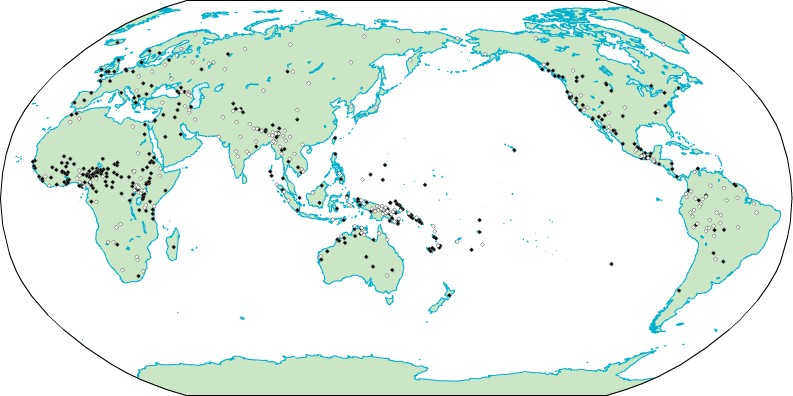
\includegraphics[height=.35\textheight]{figures/10_DistributionDefArticles}
\caption{Distribution of definite articles (black symbols) in a sample of 566 languages \citep{Dryer2005}.}
\label{map:8}
\end{figure}
%\end{styleFigureCaption}
 
%\begin{styleFigureCaption}
\begin{figure}
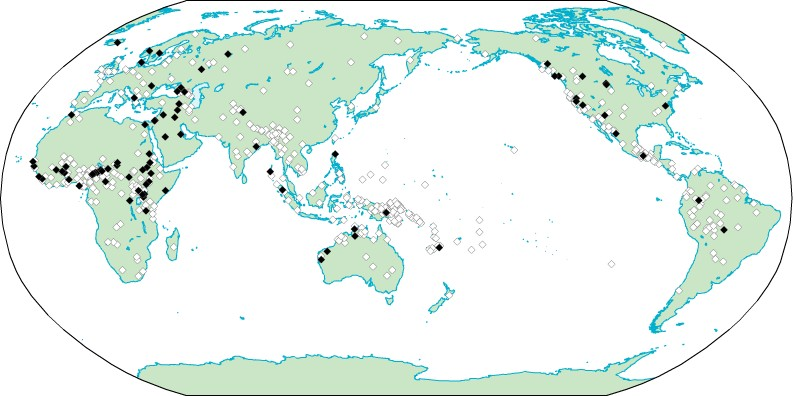
\includegraphics[height=.35\textheight]{figures/11_DistributionDefAffixes}
\caption{Distribution of definite affixes (black symbols) in a sample of 566 languages \citep{Dryer2005}.}
\label{map:8b}
\end{figure}
%\end{styleFigureCaption}

\ea 
	\gl	\label{bkm:Ref93745057}In the street, I saw a cat and a dog. The dog was barking furiously.\footnote{ It is perhaps symptomatic that examples of the anaphoric use of definite noun phrases in the literature tend to contain antecedents which are parts of a conjoined noun phrase: at least in natural speech, pronouns tend to be preferred to full noun phrases as straightforward anaphors in most contexts, and we need a structure such as a conjoined NP for there to be two equally possible antecedents, in which case a definite NP is motivated.}
\z 
\ea 
	\gl	\label{bkm:Ref93745078}I met the author of \textit{Syntactic Structures}.
\z 
\ea 
	\gl \label{bkm:Ref93745091}Please close the door. 
\z 

A highly frequent phenomenon is the “anchoring” of a definite noun phrase to some other element, whether mentioned in the discourse or not (\citealt[25]{Fraurud1992}). In \REF{6}, for instance, \textstyleLinguisticExample{the hard disk} is understood as the hard disk of the computer mentioned in the first clause – in other words, the computer serves as the anchor.  This example illustrates what is often called “associative” or “bridging co-reference”\footnote{ Another term that is sometimes used is “bridging anaphora”. Originally, the term “bridging” referred to the “bridging assumption” that provided the link between the definite noun phrase and its anchor. Thus, in (i) we have to make the assumption that the picnic supplies included beer (\citealt{ClarkEtAl1974}):\par (i) Mary got some picnic supplies out of the car. The beer was warm. \par But the point that the interpretation of definite noun phrases sometimes involves inferencing gets lost if the term “bridging” is generalized to cases where the assumption in question is trivial or follows from the meaning of the noun phrases involved. In \textit{In this group, the members work well together}, the only assumption necessary to link \textit{the members} to \textit{this group} is that a group has members. } uses of definite noun phrases,

\ea
	\gl	\label{bkm:Ref75942712}I have to fix my computer: there is some problem with the hard disk. 
\z 

In addition to straightforward referential cases as the ones exemplified above, definite articles are also used in generic noun phrases, as in \REF{7}. 

\ea 
	\gl	\label{bkm:Ref123549675}The lion is a mammal.
\z 

In English, this phenomenon is somewhat restricted, but as we shall see below, it plays a more salient role in other languages.

The most common diachronic source for definite articles is demonstrative pronouns, typically distal ones (‘that’). As pointed out by \citet[332]{Lyons1999}, there is a substantial overlap between the domains of use of demonstratives and definite articles, notably in anaphoric function. For instance, in a context like the following, both \textstyleLinguisticExample{that} and \textstyleLinguisticExample{the} are acceptable:

\ea 
	\gl Last year, I saw a film by Ingmar Bergman. I would like to see that/the film again.
\z 

The first stage in the development of definite articles from demonstratives, accordingly, consists in a more general use of a demonstrative in anaphoric function. Such “anaphoric articles” are attested in various languages – \citet[53--54]{Lyons1999} mentions Hausa and Lakota as examples. Geographically closer to the area studied here is spoken Finnish, where at least in some varieties the demonstrative \textstyleLinguisticExample{se }tends to be used in ways suggestive of an “anaphoric article” (see \citet{Laury1997} and, for a more sceptical view, \citealt{Juvonen2000}:

\ea%\label{}
\langinfo{Finnish}{}{}\\
\gll	...niin  sit  \textbf{se} mies  meni  ja,\\
		so  then  \textbf{this} man  go.{\pst}  and\\
\gll	osti  \textbf{ne} kaikki  ilmapallot\\
		buy.{\pst}  \textbf{this.{\pl}} all  balloon.{\nom}.{\pl}\\
\gll	ja  anto  ne  \textbf{sille} pojalle,\\
		and  give.{\pst}  this.{\pl}  \textbf{this.{\all}} boy.{\all}\\
		
\gll 	ja  sit  \textbf{se} poika...\\
		and then  \textbf{this} boy\\
\glt 	‘…so then the man went and bought all the balloons and gave them to the boy, and the boy…’ (\citealt[136]{Juvonen2000})

\z

For an erstwhile demonstrative to look more like the definite articles we are used to from languages such as English, it has to acquire also non-anaphoric uses. Finnish \textstyleLinguisticExample{se }is still unacceptable e.g. in a context as that exemplified in \REF{6}. The mechanism behind an expansion from an anaphoric to a more general definite article is not well understood, but we may note that it involves the elements usually associated with grammaticalization processes: a rise in frequency through the expansion to new contexts where the element becomes obligatory, combined with a loss of prosodic prominence and an ensuing reduction of phonetic weight (what is commonly but misleadingly referred to as “erosion”). 

A language can also have more than one definite article. One way in which such a situation can develop is through separate waves of grammaticalization that give rise to a “layered” system in which two (or more) elements of varying age compete with each other. The youngest element will then typically have the functions that are first to grammaticalize, such as anaphoric ones. This is exemplified by various West Germanic varieties, such as the Fering dialect of North Frisian described by \citet{Ebert1971} (although the actual rules for choosing between the articles are a bit more complicated; for an accessible account see \citealt[162]{Lyons1999}). Compare the following examples:

\ea%\label{}
\langinfo{North Frisian (Fering dialect)}{}{}\\
\ea 
	\gll 	Hat  kaam  me  \textbf{a} \textbf{maan}.\\
			she  come.{\pst}  with  \textbf{{\deff}} \textbf{man}\\
	\glt 	‘She came with her husband, lit. the man.’
\ex
	\gll	Hat  kaam  me  \textbf{di} \textbf{  maan}.\\
			she  come.{\pst}  with  \textbf{{\deff}} \textbf{man}\\
	\glt	‘She came with the man.’ (\citealt[163]{Lyons1999})

	\z 
\z

Among languages whose definite articles would seem to be of a “garden variety” kind, there is in fact considerable variation which is largely attributable to how far the grammaticalization process has gone and which routes it has taken. For example, the English definite article on the whole has a relatively restricted domain of use compared to definite articles in many other languages. Most saliently, as has already been noted, English has a restricted use of definite articles w\textstyleBodytextCChar{i}th generic noun phrases – this will be further discussed in section \sectref{sec:3.2.1}. But English also shows a reluctance to use articles with proper names, in contrast to many other languages, such as Greek and southern German vernaculars, but also many northern Scandinavian vernaculars, to be discussed in section \sectref{sec:3.2.8}. Even in English there are exceptions, such as some types of geographical names, e.g. names of rivers such as \textstyleLinguisticExample{the Thames}. Since proper names are usually seen as “inherently definite”, the use of definite articles would seem to be wholly redundant from the communicative point of view. However, such apparently redundant uses of grammatical elements are typical of later stages of grammaticalization processes and show that the identification of the “function” of a grammatical element is not always easy (\citealt[81--86]{Dahl2004}). 

The story does not end here, however. A definite article may develop further, expanding its domain of use to a point where it is no longer possible to call it “definite” or even an “article”. This process was described by \citet{Greenberg1978}, who argued that definite articles are the source of various grammatical morphemes.  A particularly notable example of this process involves noun class markers, such  as those found in Bantu languages wherein the affixes are obligatory with nouns irrespective of the context in which they appear. The details of the route to such a situation from “garden variety” definite articles are far from clear. One example of an intermediate stage suggested by Greenberg would be the “specific” articles found in many Oceanic languages which also cover many of the functions of the indefinite article of English, in particular that of introducing new, specific discourse referents. Compare the Samoan article \textstyleLinguisticExample{le} in the following example: 

\ea%\label{}
\langinfo{Samoan (Austronesian)}{}{}{}{}\\
\gll	ʽO  \textbf{le} ulug\=aliʽi,  f\=anau  \textbf{l}{}-a  l\=a  tama\\
		{\prs}  \textbf{{\art}} couple  give\_birth  \textbf{{\art}}{}-{\poss}  3{\du}  child\\
\gll	ʽo  \textbf{le} teine  ʽo  Sina.\\
		{\prs}  \textbf{{\art}} girl  {\prs}  Sina\\
\glt ‘There was \textbf{a} couple who had \textbf{a} child, \textbf{a} girl called Sina.’ (\citealt[259]{HovdhaugenEtAl1992})

\z

What we find in Scandinavian vernaculars, however, is an expansion of the range of uses of definite articles that goes in a different direction and cannot be described in terms of “specificity” in any sense. The Scandinavian development therefore is of considerable interest for our understanding of the role of definite articles in grammaticalization processes.

\begin{figure}[h]

%\begin{styleBeschriftung}
\includegraphics[height=.5\textheight]{figures/12_Definiteness}
\caption{Definiteness marking of non-modified nouns in Europe west of 30°E (dark grey: free article only, light grey: suffixal marking).}
\label{map:10}
\end{figure}



\subsection{Definite marking in Scandinavian in general}
\label{sec:3.1.4}

As already noted, Western Europe is one of the areas in the world where definite articles are generally present. The distribution is determined by areal rather than by genetic factors. Although definite articles would seem to be a general feature of the Germanic, Celtic and Romance families, this is a late phenomenon not found in the older historical stages of Indo-European. The presence of definite articles in these languages must therefore be attributed to a later spread rather than to inheritance from a parent language. In fact, there is a relatively neat diachronic progression in the appearance of definite articles from the Eastern Mediterranean to north-western Europe, basically in the order of Semitic → Greek → Romance → Germanic, suggesting a rather slow expansion wave which took about two thousand years to complete. The Fenno-Ugric and Slavic languages in Europe are split with respect to definiteness marking, and there is evidence that definite articles are latecomers in these languages also

If we focus on Europe west of 30°E (\figref{map:10}), we find definite articles in one central and two relatively peripheral areas. In the large central area comprising most of Western Europe, definite articles are manifested as free morphemes occurring initially in noun phrases. However, in the two peripheral areas found in Scandinavia and the Balkans, definiteness is marked by suffixing.  This marking occurs in the standard languages of Romanian, Bulgarian, Macedonian, and Albanian. These developments fit less straightforwardly into the general expansion pattern, although the general timing and the closeness to the preposed article area makes areal influence likely here, too. In Scandinavia, the situation is further complicated by the presence of both preposed and suffixed articles, with varying divisions of labour in the individual languages (see \sectref{sec:4.3} for details). It should also be noted here that there are significant differences between the suffixed articles in Scandinavia and those found in the Balkans: the latter should probably be seen as movable clitics rather than suffixes – they typically show up on the first word in the noun phrase, more or less irrespective of its grammatical category (thus, in Macedonian and Bulgarian, definite articles can be cliticized even to possessive pronouns: \textstyleLinguisticExample{moja-ta kniga} ‘my-{\deff} book’). 

The origins of definiteness marking in the Scandinavian languages are rather obscure. Definite articles seem to have been absent from the earliest stages of Old Nordic and there are only sporadic attestations from runic inscriptions. From Sweden, two attestations of what seems to be the same formulaic phrase \textstyleLinguisticExample{kuþ heabi onti-ni }or\textstyleLinguisticExample{ kuþ hialbi *anti-ni} ‘God help soul.{\deff}’ i.e. ‘may God help the soul’ are cited. When written documents start to appear in the 13\textsuperscript{th} and 14\textsuperscript{th} centuries, both preposed and suffixed articles are still rare in many texts, in particular in laws and poetry (which happen to constitute the bulk of the preserved written material); such instances are possibly rarer in Denmark and Sweden than in the West Nordic area. Here are some statistics (\citet[938]{Delsing2002}, based on \citet{Larm1936} and \citealt{Skautrup1944}: 

%\begin{styleTableCaption}
\begin{table}
\caption{ Percentage of definite nouns among nouns in general}
\label{tab:1}
\begin{tabular}{ll}
 \lsptoprule
Older Västgöta Law  & 0.5
\\
Uppland Law & 5
\\
Östgöta Law&  7.5
\\
Scanian Law & 8
\\
Jutland Law & 10
\\
\lspbottomrule

\end{tabular}

\end{table}
%\end{styleTableCaption}

The source of the suffixed article is commonly assumed to be an original demonstrative \textstyleLinguisticExample{inn} or \textstyleLinguisticExample{hinn}. The forms with an initial \textstyleLinguisticExample{h-}, which may be due to a reinforcement of \textstyleLinguisticExample{inn} in analogy with other 3\textsuperscript{rd} person pronouns (\citealt[135]{Perridon1989}, \citealt[723]{Syrett2002}) were only used in preposed position in East Nordic. According to a popular hypothesis (going back to Grimm (1822--40), the suffixed article originated as an adjectival article in a construction such as \textstyleLinguisticExample{maþr inn gamli }‘man the old’. I think this hypothesis should be viewed with some scepticism. The low frequency in spoken language of the adjectival construction makes it unlikely as a general model for noun phrases (as is also noted by \citealt[63]{SaltveitEtAl1971}). There also seems to be little concrete evidence of such a development anywhere. (In the Balkan languages the corresponding constructions would be expressed as ‘man-the old’ and the article would thus not be in the right place relative to the noun.)  Thus, the alternative hypothesis that the suffixed article has developed out of an unstressed postposed demonstrative seems more plausible.  In fact, this phenomenon is exemplified by the inscription \textstyleLinguisticExample{hali hino} ‘[flat] stone \textstyleLinguisticExample{this}’ on the whet-stone of Strøm (Norway) from about 600 \textsc{C.E.} 

With respect to the timetable for the development of the suffixed article, there seem to be two basic views. The first, which assumes that the genesis of the suffixed article in the spoken language is significantly earlier than its appearance in the written language, appears to originate with \citet{Neckel1924}.  This position is also taken in recent works by both \citet[142]{Perridon1989}, who speaks of “a hidden life” of the article “before it starts its public written life”, and \citet[723]{Syrett2002}, who says that “…it seems reasonable to suggest that” the suffixed article “was the end product of an unrelated series of morphological and syntactical developments within the progression from” Ancient Norse to Old Norse (the transitional period between these two being broadly defined as lasting from the 6\textsuperscript{th} century until 1100). 

The main representative of the other view is \citet[938--939]{Delsing2002} who thinks that the suffixed article “developed as an innovation in the 13\textsuperscript{th} century”. (He does not say explicitly what territory this claim is intended to cover, but it is given in the context of a treatment of Old Swedish and Old Danish.) He argues against the view that “the low frequency of articles in the oldest texts can be explained by style”, pointing to the fact that not only legal and poetic texts but also texts which “are written in styles where we would expect an ample use of the articles”,  e.g. the Gutasaga (a text presumed to be from the 13\textsuperscript{th} century and containing a description of the mythical origin of the island of Gotland) and the chronicles from Vidhem [S47], have a low frequency of definite marking. 

Delsing’s discussion of the style question seems to conflate two possible effects of style (or genre) on the use of definite articles: (i) a generally lower frequency of definite marking due to pragmatic reasons; (ii) the possible use of an archaizing language. Thus, he says: “Runic inscriptions, laws and poetry are not the kind of texts where we expect to find articles” (ibid.). There obviously are some text types where definite articles would be infrequent in any language due to a restricted need for definite reference, and runic inscriptions may be cases in point, but this would hardly hold for the other kinds of text mentioned by Delsing. Thus, in a language where definite articles are regularly used, such as English or Modern Swedish, they occur also in laws and poetry. Consider as an example Article 1:1 of the Swedish constitution (\textstyleLinguisticExample{Regeringsformen}), which contains two noun phrases with definite marking:

\ea%\label{}
\langinfo{Swedish}{}{}{}{}\\
\gll 	\textbf{Den} \textbf{  offentliga} \textbf{  makten} utövas  under  \textbf{lagarna}.\\
		\textbf{{\deff}} \textbf{public} \textbf{power.{\deff}} exert.{\pass}.{\prs}  under  \textbf{law.{\pl}.{\deff}}\\
\glt  ‘(The) public power is exerted under the laws.’

\z

On the other hand, laws and poetry are genres which are often formulated in an archaizing language and which may thus differ significantly from other text types and in particular from informal spoken language. It may be noted that even contemporary legal Swedish exhibits patterns of article usage which most probably reflect an older stage of development. Thus, until the last decades of the 20\textsuperscript{th} century, it was normal for singular generic noun phrases in legal texts to be used without any article, as in 

\ea%\label{}
\langinfo{Swedish}{}{}{}{}\\
\gll	\textbf{Hund} skall  hållas  kopplad  på  \textbf{offentlig} \textbf{  plats}.\\
		\textbf{dog} shall  keep.{\pass}.{\inf}  leash.{\pp}  on  \textbf{public} \textbf{place}\\
\glt ‘A dog shall be kept on a leash in public places (lit: Dog shall be kept leashed on public place)’

\z

The absence of definite articles in medieval legal prose would thus be due to an archaizing language rather than to the general low frequency of definite articles in legal texts. The same goes for poetry, mutatis mutandis. But as Delsing points out, there are other texts which also exhibit a low incidence of definiteness marking. The first text mentioned by Delsing, the Gutasaga, may not be too relevant in this context, since the variety it is written in, Old Gutnish, is not necessarily representative of mainstream Old Swedish.  On the other hand, the Vidhem chronicle (presumed to be written in Västergötland around 1250, although there seems to be no general agreement on this) may be evidence that the use of definite marking was generally restricted in the written language of the period. However, this text is an appendix to the Västergötland law, so one could perhaps expect the style to be close to that of legal language. 

In my opinion, several things speak against the hypothesis that the suffixed article is a 13\textsuperscript{th} century innovation. One is the geographical distribution of the suffixed article: in spite of its low frequency in some early texts, it is attested in the 13\textsuperscript{th} century from all parts of the Scandinavian area: Iceland, Norway, Denmark, and Sweden.  And even earlier, in the first half of the 12\textsuperscript{th} century in Iceland (according to \citealt[§1019]{Perridon2002}), there is a consistent use in the First Grammatical Treatise. Moreover, although not frequent, even the very earliest texts in Sweden do contain quite a few definite articles. Thus, the Older Västgöta Law, assumed to be from around 1225, contains 23 instances of suffixed articles (\citealt[24]{Larm1936}). This means that, already at this stage, the suffixed article was well enough entrenched to show up in written language all over Scandinavia, although it was still used in a restricted fashion. 

Furthermore, if it were the case that the forms that we see in the oldest texts represent a recent innovation, we would expect them to behave in a way typical of early stages of a grammaticalization process. This is not the case, however. When we first meet the suffixed definite article, it has already reached a relatively advanced stage of grammaticalization. This goes both for form and function: even the earliest attestations are suffixed rather than separate words, and they display non-anaphoric uses (see \sectref{sec:3.1.3}), suggesting a full-fledged definite article. For instance, the earliest attestations from Sweden, \textstyleLinguisticExample{kuþ hialbi antini }‘God help the [i.e. his] soul’ are clear examples of an associative use. The following example from the Vidhem chronicles is also clearly non-anaphoric:

\ea%\label{}
\langinfo{Medieval Written Swedish}{}{}{}{}\\
\gll 	Han  læt  gøræ  \textbf{kyrkiunæ} i  agnistaðhum.\\
		he  let.{\pst}  make.{\inf}  \textbf{church.{\deff}.{\acc}} in  Agnestad\\
\glt 	‘He had the church in Agnestad built.’ [S47]

\z

If the rise of definite articles was close in time to the creation of the documents in which they are common, we would expect to find more signs of the early stages of development, both with regard to form and to function.

What was just said about the earliest documented stages is paralleled in the modern forms of Scandinavian: there is no variety that reflects an earlier stage in the grammaticalization process. It should also be noted that the suffixed article has a virtually total coverage in Scandinavian, with the exception of the Jutish dialects in Denmark that use prefixed articles exclusively. Thus, the suffixed articles are also manifested in a remarkably uniform way in the most conservative and peripheral varieties. This is in contrast to the prefixed definite article, which is absent both in modern spoken Icelandic and in the Peripheral Swedish vernaculars, and the indefinite article, which is absent in Icelandic. It is also in contrast to most of the major phonological changes in medieval Scandinavian, which tended to be only partially implemented or not implemented at all in peripheral areas. An example is the monophthongization of the original diphthongs \textstyleLinguisticExample{ai} and \textstyleLinguisticExample{au }to\textstyleLinguisticExample{ e }and\textstyleLinguisticExample{ ö,} respectively,\textstyleLinguisticExample{ }which according to the standard view spread from Denmark to south and central Sweden in the 11\textsuperscript{th} century, but which a millennium later has still not yet been completed in some of the outlying areas, such as northern Norrland, western Dalarna, Österbotten and Gotland.  

\subsection{ Neutralization of the definite-indefinite distinction}
\label{sec:3.1.5}

A fairly common phenomenon, which should be kept apart from the expansion of the definite forms discussed in this chapter, is the partial neutralization of the opposition between definite and indefinite forms: that is, the same form comes to represent both definite and indefinite. For instance, in Orsa (Os), neuter nouns do not distinguish definite and indefinite forms. There is no vernacular in which the neutralization between indefinite and definite is total. Rather, as in Orsa, it tends to hit paradigms only partially. What forms are neutralized varies from place to place, but there are a few typical patterns.

\subsubsection{Neutralization between indefinite and definite in the plural}
 This is probably the most common pattern, being found in relatively many places. 

In Ovansiljan, this appears to be a relatively late development. \citet{Levander1909} describes Elfdalian as still having a distinction for masculine nouns in the nominative plural, e.g. \textstyleLinguisticExample{kaller:kallär }(indefinite and definite nominative plurals of \textstyleLinguisticExample{kall }‘man’), and for some feminine nouns, e.g. \textstyleLinguisticExample{djieter:djietär} (from \textstyleLinguisticExample{djiet} ‘goat’), but not for a feminine noun such as \textstyleLinguisticExample{flugu }‘fly’ which has the only form \textstyleLinguisticExample{flugur} in the nominative plural. However, Levander notes that the distinction is not found in all villages in Älvdalen (with varying isoglosses for different types of nouns), and according to \citet[170]{Levander1928}, it is found in Orsa and Våmhus but not in Mora, Sollerön, Venjan and Ore. In the accusative plural, a distinction between forms such as \textstyleLinguisticExample{kalla:kalla; }exist in all the varieties which retain the nasal vowels, that is, most of Älvdalen, Våmhus and Bonäs (Mora parish). 

In Karleby\footnote{ The previous town of Gamlakarleby and the parish of Karleby were merged into Karleby town in 1977. For simplicity, I use the name “Karleby” throughout. } (NOb), the old indefinite plural forms have disappeared entirely in favour of the definite ones, e.g. \textstyleLinguisticExample{gåǣ7a} ‘(the) yards’, \textstyleLinguisticExample{gatuna} ‘(the) streets’ (\citealt[93]{Hagfors1891}). Likewise, in Runö (Es), there is no indefinite-definite distinction at all in the plural (cf. \REF{69} below.)

Neutralization between indefinite and definite in neuter nouns, with zero endings in the nominative/accusative, is found in at least three geographically quite distinct areas: Orsa and northern Venjan in the Ovansiljan area (\citealt[133]{Levander1928}) and parts of Värmland. In the Cat Corpus we thus find the following examples of cognates of Swedish \textstyleLinguisticExample{golv} ‘floor’ used as a definite noun with a zero ending:

\ea%\label{}
\langinfo{Orsa (Os)}{}{}{}{}\\
\gll	\textbf{Gow} wa  niskajrad.\\
		floor  be.{\pst}  new-clean.{\pp}\\
\glt 	‘The floor was newly cleaned.’ (Cat Corpus)

\z

%\begin{styleTextkrper}
(cf. Swedish \textit{Golvet var nyskurat}) 

%\end{styleTextkrper}

\ea%\label{}
\langinfo{Västra Ämtervik (Vm)}{}{}{}{}\\
\gll	Men  nepå  \textbf{gôLv} va  dä  en  hög  mä  matt-traser.\\
		But  down\_on  \textbf{floor} be.{\pst}  it  {\indf}  heap  with  carpet\_rag.{\pl}\\
\glt	‘But on the floor there was a heap of rags.’ (Cat Corpus)

\z

%\begin{styleTextkrper}
(cf. Swedish \textit{Men på golvet var det en hög mattrasor})

%\end{styleTextkrper}

In Orsa and Venjan, where the dative case is still alive, there is also neutralization in the dative of these nouns. 

\subsubsection{Neutralization between indefinite and definite in the dative}
 This appears to be common or even normal in the dative-preserving vernaculars. Thus, according to \citet{Marklund1976}, nouns in \textit{Skelletmål} have two rather than four dative forms – one for singular and one for plural, as in \textstyleLinguisticExample{pigen} ‘the maid’: \textstyleLinguisticExample{pigåm} ‘the maids’ (from \textstyleLinguisticExample{piig} ‘maid’), or just one for both, as in \textstyleLinguisticExample{vaidjåm }‘the wall(s)’. There is thus no definite:indefinite distinction, and although Marklund does not say so explicitly, it appears that the normal interpretation of the dative forms is definite – the ending is also normally added to the definite stem (as in the case of \textstyleLinguisticExample{vaigg}:\textstyleLinguisticExample{vaidjåm}).

The developments are somewhat different in the singular and the plural. In the singular, the indefinite form tends to be marginal or absent, whereas the definite form is stronger; in the plural, it is the definite form that disappears. In Dalecarlian,  the vernacular of Orsa appears to be the only exception in that there are separate forms for definite dative plurals ending in \nobreakdash-\textstyleLinguisticExample{uma, }as in \textit{revuma} ‘fox.{\pl}.{\deff}.{\dat}’. According to \citet{Levander1909}, at the time of his investigation in the first decade of the 20\textsuperscript{th} century, elderly persons in Älvdalen sometimes used definite dative plurals in\textstyleLinguisticExample{ }\textstyleLinguisticExample{\nobreakdash-ume}.  Otherwise, the indefinite dative plural ending \textstyleLinguisticExample{\nobreakdash-um} has been generalized, e.g. Elfdalian \textit{rövum} ‘fox.{\pl}.{\deff}.{\dat}’.

\subsubsection{Neutralization of definiteness in individual lexemes}
Individual lexemes or groups of lexemes sometimes have identical indefinite and definite forms. Thus, in Elfdalian, neuter nouns in \textstyleLinguisticExample{\nobreakdash-ð }have a zero ending in the definite singular nominative and accusative, e.g. \textstyleLinguisticExample{broð} ‘bread’. Many Elfdalian nouns are not inflected at all.  The word for ‘coffee’ is perhaps most notable in this connection; \textstyleLinguisticExample{kaffi}, which like \textstyleLinguisticExample{broð} is highly frequent in contexts in what is below called non-delimited readings, would normally trigger a definite form. 

Neutralization of the definiteness distinction means that the consequences of the changes discussed below are more restricted than they would otherwise be, since in many cases it will not make any difference if an indefinite or a definite form is chosen. It also means that direct comparisons between dialects are not always possible – if you translate an example from one dialect to another, the distinction between definite and indefinite may disappear on the way. 

As I said above and as also argued by \citet{Hummelstedt1934}, neutralization of the definiteness distinction is in principle a different phenomenon from that of extensions of the domain of definite forms. One may of course also speculate whether there is any causal relationship between the processes by which definite forms acquire new uses and the processes by which definite and indefinite forms are neutralized. What could perhaps be expected is that if the definite forms expand too much, the indefinite forms will simply fall into oblivion. This is essentially what seems to happen in the final stages of the grammaticalization paths described by Greenberg. However, confusingly, it is not always the definite forms that win out in the neutralization process: for instance, in Orsa, as we have seen, neuter nouns have zero endings for both indefinite and definite. In other words, the neutralization process may well obliterate the results of the grammaticalization process. On the other hand, given that neutralization is so common, it is somewhat remarkable that speakers are still able to make the distinction when it is needed. Also, there is no consistency in the neutralizations: thus, Orsamål is “radical” in having no definiteness distinction in neuter nouns and “conservative” in being the only vernacular that preserves the same distinction in the dative plural.

It should also be noted that the systems described above often go against general assumptions about markedness relations in morphology (as when a distinction is upheld in oblique cases but not in the nominative) (see \citealt{DahlEtAl2006}).

\section{ Survey of extended uses of definites}
\label{sec:3.2}\subsection{ Generic uses}
\label{sec:3.2.1}

Generic noun phrases are used to refer generally to a species (natural kind), class or type of entities.\footnote{ In Swedish grammatical literature, the traditional term used is “allmän betydelse” ‘general meaning’.} There are actually at least two main kinds of generic uses of noun phrases (\citealt[19]{KrifkaEtAl1995}). The first, and most well-known, is when the noun phrase occurs in a context in which a general, “law-like” or nomic statement is made about the species, class or type that the noun phrase denotes (\citealt{Dahl1973}. The\textbf{ }standard example in the linguistic literature is \textstyleLinguisticExample{Beavers build dams}, in which dam-building is described as a typical activity of beavers. This first type is called “characterizing sentences” by \citet{KrifkaEtAl1995}. In the second type, which they call “kind predications”, the species or kind is referred to without there being a generalization over its members. For instance, in the sentence \textstyleLinguisticExample{The zoologist was studying the beaver}, the beaver species is referred to as the object of the zoologist’s study, but no inference can be drawn about individual beavers.

An interesting typological generalization is that generic uses of noun phrases do not in general have a dedicated mode of expression; rather, several different types of noun phrases may be recruited for those uses. Thus, in English, bare plurals, singulars with indefinite articles, and singulars with definite articles can all be used generically. We may thus also say \textstyleLinguisticExample{A beaver builds dams} and \textstyleLinguisticExample{The beaver builds dams}. There are quite definite restrictions, however. Indefinite singulars can only be used for “characterizing sentences”, not for “kind predications”: \textstyleLinguisticExample{The zoologist was studying a beaver }must mean that he or she was studying a concrete individual (or, possibly, a specific sub-species). Also, in English, definite plurals and definite mass nouns cannot in\textbf{ }general be used generically: \textstyleLinguisticExample{The beavers build dams} must refer to a specific group of beavers and \textstyleLinguisticExample{The gold is expensive} must refer to a specific mass of gold. In this respect, languages with definite articles vary quite considerably. To see this, it is sufficient to compare English to French, where in fact \textstyleLinguisticExample{Les castors construisent des barrages} is the standard way of saying that beavers build dams, and correspondingly, the articleless construction, which is typical of English, is generally ungrammatical. In fact, the French situation appears to be more common among languages with definite articles (at least in Europe). That is, plurals and mass nouns as a rule take a definite article when used generically. \citet{Behrens2005} looked at five European languages – French, English, German, Greek, and Hungarian, and found that French, Greek and Hungarian all behave similarly in this regard, whereas German turned out to be somewhere in the middle. Compare the following example from Behrens’ corpus, \textstyleLinguisticExample{The Little Prince}:

\ea
	\ea {
	\gl English: Flowers are weak creatures.
	}
	\ex {
	\gl German: Die Blumen sind schwach.
	}
	\ex {
	\gl French: Les fleurs sont faibles.
	}
	\ex {
	\gl Greek: Ta lulúdhja íne adhínama.
	}
	\ex {
	\gl Hungarian: A virágok gyengék.
	}
	\z 
\z

%\end{styleExLtrTblii}

%\end{listLFOcvileveli}

Swedish, like German, is an intermediate case in that it sometimes follows the French and sometimes the English pattern. Thus, Swedish uses a definite NP in \textstyleLinguisticExample{Livet är kort} ‘Life is short’ (cf. French \textstyleLinguisticExample{La vie est brève}) but like English prefers a bare noun in \textstyleLinguisticExample{Guld är dyrt} ‘Gold is expensive’. Possibly, Swedish is slightly more restrictive than German in the use of definite generics: it would seem more natural to use an indefinite plural in the translation of \REF{17} than a definite one:

\ea%\label{}
\langinfo{Swedish}{}{}{}{}\\
\gll	\textbf{Blommor} är  veka  varelser.\\
		\textbf{flower.{\pl}} be.{\prs}  weak.{\wk}  being.{\pl}\\
\glt	‘Flowers are weak beings.’

\z

However, many Peripheral Swedish varieties behave more like French in this respect, with an across-the-board use of definite forms in generics. We thus find examples such as the following:

\ea%\label{}
\langinfo{Älvdalen (Os)}{}{}{}{}\\
\gll	\textbf{Guld} \textbf{ið} ir  dyrt.  \\
		\textbf{gold.{\deff}} be.{\prs}.{\sg}  expensive.{\n}  \\
\glt	‘\textbf{Gold} is expensive.’ (questionnaire)

\z

Generic uses of definites seem to be among the most widespread of the extended uses of definites found in the Peripheral Swedish area. They are thus characteristic not only of Upper Norrland and Upper Dalecarlian but also of regions such as Värmland, southern Finland, and Norway. Compare the following examples:

\ea%\label{}
\langinfo{Östmark (Vm)}{}{}\\
\gll	\textbf{Kaffen} \textbf{ä} \textbf{  allt} \textbf{  bätter} \textbf{  än} \textbf{ten}.\\
		\bfseries coffee.{\deff}  be.{\prs}  sure  better   than  tea.{\deff}\\
\glt	‘Coffee is sure better than tea.’ (\citealt{Broberg1936}

\z

\ea%\label{}
\langinfo{Pernå (Ny)}{}{}\\
\gll	\textbf{Björc(in,} han  ä  nɷ  bäter  ti  m\={ö}bler,\\
		\textbf{birch.{\deff}} it  be.{\prs}  surely  better  for  furniture.{\pl}\\
\gll 	men  han  ä  so  h\=order  ti  arbita.\\
		But  it  is  so  hard  {{\inf}m}   work.{\inf}\\
\glt	‘Birch, it is better for furniture, but it is so hard-worked.’ (Lundström (1939: 13--14)

\z

\ea%\label{}
\langinfo{Ingå (Ny)}{}{}\\
\gll	Va  hadde  man  för  tjö:rdo:n  ti  de:?  {}-  \textbf{Tjärran}.\\
		what  have.{\pst}  one  for  vehicle  for  that    \textbf{cart.{\deff}}\\
\glt	‘What kind of vehicle did they use for that? – A [lit. the] cart.’ (\citealt[42]{Harling-KranckEtAL1998})

\z

\ea%\label{}
\langinfo{Tromsø (Troms, Norway)}\label{bkm:Ref135628619}{}{}\\
	\ea
		\gll	Det  e  mer  varme  i  \textbf{kola} enn  i  \textbf{veden}.\\
				It  be.{\prs}  more  heat  in  \textbf{coal.{\deff}} than  in  \textbf{firewood.{\deff}}\\
		\glt	‘There is more heat in coal than in firewood.’ (\citealt[19]{Iversen1918})

	\ex
		\gll	\textbf{Ulvan} e’  minder  som  \textbf{bjørnan}.\\
				\textbf{Wolf.{\deff}.{\pl}} be.{\prs}  small.{\cmpr}  than  \textbf{bear.{\deff}.{\pl}}\\
				
		\glt	‘Wolves are smaller than bears.’ (\citealt[18]{Iversen1918})
	\z 
\z

The examples in \REF{23} are the only ones that I have found in the literature from Norway, but reactions from Norwegian linguists suggest that such generic uses are in fact more widespread. 

As noted above, Delsing’s “tentative” map of the “partitive” uses of definites in Scandinavia shows all of Northern Sweden (and a strip in Norway along the Swedish border in Trøndelag) as having “partitive articles where the standard language has generic naked forms”, the southern border coinciding more or less with the \textstyleLinguisticExample{limes norrlandicus.} More specifically, it passes through northern Värmland and southern Dalarna and cuts Gästrikland in two. As for Värmland, Delsing’s line is roughly at the height of Torsby and Ekshärad, but the Cat Corpus examples – from Västra Ämtervik (Fryksdalen) and Mangskog – give evidence that the border goes at least 40--50 kilometers further south in Värmland: 

\ea
	\ea { %\label{}
	\langinfo{Västra Ämtervik (Vm)}{}{}\\
	\gll	\bfseries FôggLân  skâ  en  fôll  int  mat…\\
			\bfseries bird.{\pl}.{\deff}  shall.{\prs}  one  {\prag}  {\neg}  feed\\
	}
	\ex {
	\langinfo{Mangskog (Vm) }{}{}\\
	\gll	\bfseries Fugglane  skâ  en  föll  inte  mate…\\
			\bfseries bird.{\pl}.{\deff}  shall.{\prs}  one  {\prag}  {\neg}  feed\\
	\glt 	‘Birds, you should not feed…’ (Cat Corpus)
	}
	\z 
\z

%\begin{styleTextkrper}
The use is not consistent, however – in the following example the indefinite form is used:

%\end{styleTextkrper}

\ea%\label{}
\langinfo{Västra Ämtervik (Vm)}{}{}\\
\gll 	\textbf{Sockerkak} ä  dä  bäst  Kâtt’n  vet.\\
		\textbf{Sponge\_cake} be.{\prs}  {\deff}.{\n}  best  cat.{\deff}  know.{\prs}\\
\glt ‘Sponge cake is Cat’s favourite.’ (Cat Corpus)

\z

\ea%\label{}
\langinfo{Mangskog (Vm)}{}{}\\
\gll 	\textbf{Sockerkake} ä  dä  bäste  Katten  vet.\\
		\textbf{Sponge\_cake} be.{\prs}  {\deff}.{\n}  best  cat.{\deff}  know.{\prs}\\
\glt 	‘Sponge cake is Cat’s favourite.’ (Cat Corpus)

\z

On the other hand, there is rather little evidence for generic uses of noun phrases in the rest of Delsing’s southern area. Delsing does not himself provide any such examples, and the Cat Corpus evidence is rather negative, in the following sense: In the translations of \REF{24}{}-\REF{25}, no definite forms show up in texts from Hälsingland (3 texts), Härjedalen (1 text), and Dalarna outside the Ovansiljan area (about ten texts). (The examples from Ovansiljan are sometimes ambiguous due to the neutralization of the definiteness distinction in the plural.) Consider, for example, the following three translations from Hälsingland:\footnote{ The endings in the plural tend to be confusing – for instance, the -a ending is definite in some vernaculars and indefinite in others. In the case of Färila and Järvsö the indefinite plural of ‘bird’ is \textit{fôggla} and the definite plural is \textit{fôgglan}. }

\ea
	\ea{
	\langinfo{Färila (Hä)}{}{}\\
	\gll	\textbf{Fôggǣ7â} skâ  mânn  fäll  int  matâ,  häll!\\
			\textbf{Bird.{\pl}} shall.{\prs}  one  {\prag}  {\neg}  feed.{\inf}  either\\
	}
	\ex {
	\langinfo{Forsa (Hä)}{}{}\\
	\gll	\textbf{Fug}l\textbf{ar} ska  man  fell  int  mata  e.\\
			\textbf{bird.{\pl}} shall.{\prs}  one  {\prag}  {\neg}  feed.{\inf}  {\neg}\footnotemark{}\\
	}
	
	\ex{
	\langinfo{Järvsö (Hä)}{}{}\\
	\gll	\textbf{Fôggla} ska  man  fell  int  mata,  e.\\
			\textbf{bird.{\pl}} shall.{\prs}  one  {\prag}  {\neg}  feed.{\inf}  {\neg}\\
	\glt ‘Birds, you should not feed…’ (Cat Corpus)
	}
	\z 
\z

\footnotetext{ The morpheme \textit{e} is a reinforcing element that co-occurs with negation often enough to warrant talking of a double negation construction. It is common in vernacular texts from Uppland and Hälsingland.}

%\begin{styleTextkrper}
Likewise Västerdalarna:

%\end{styleTextkrper}

\ea
	\langinfo{Transtrand (Vd)}{}{}\\
	\ea {
		\gll	\textbf{Göll} e  dirt.\\
				\textbf{gold} be.{\prs}  expensive\\
		\glt 	‘Gold is expensive.’ (questionnaire)
	}
	\ex {
		\gll 	\textbf{Häster} kut  fort.\\
				\textbf{horse.{\pl}} run.{\prs}  fast\\
		\glt 	‘Horses run fast.’ (questionnaire)
	}
	\z 
\z

\subsubsection{Citation uses}
 Among uses of definite nouns that are close to generics, one can mention meta-linguistic uses or what is commonly called “citation forms”. This kind of use seems to be quite common in many parts of the peripheral area. Thus, speakers who are asked to write down word lists often quote nouns in the definite form. This use of definite forms is already reflected in the word lists of \textit{Pitemål} compiled by the philologist Johan Ihre in the 18\textsuperscript{th} century (\citealt{Reinhammar2002}. 

Some clear examples of citation uses are:

\ea %\label{} 
\langinfo{Ersmark (NVb) }{}{}\\
\gll 	He  kall  ve  fö  \textbf{sjanostn} för  gammalt.\\
		it  call.{\prs}  we  for  \textbf{sand\_cheese.{\deff}} for  old.{\n}\\
\glt 	‘This we call “sand cheese” of old.’ [S43]

\z

\ea %\label{} 
\langinfo{Svartlå, Överluleå (Ll)}{}{}\\
\gll Jö  tråo  dom  kåles  \textbf{skråkaran}.\\
I  think.{\prs}  they  call.{\pass}.{\prs}  \textbf{“skråkar”.{\deff}.{\pl}}\\
\glt ‘I think they are called “skråkaran” ‘ [S45]

\z

Definite forms in citation uses are occasionally mentioned in the literature. Thus, \citet[282]{ÅgrenEtAl1954} say that if you ask a Norrlandic farmer what the berries that grow along the sides of the field are called, he answers \textstyleLinguisticExample{Åkerbära} ‘the polar cloudberries’. According to \citet[82]{Lagman1979}, the definite form shows up “to a certain extent” as the “lexical form” in Estonian Swedish. Thus, he says, the answer to the question “What is ‘white horse’ in Nuckö Swedish?” would be \textstyleLinguisticExample{hoit aiken} ‘white horse.{\deff}’. \citet[8]{Steensland1994}, in his book on Elfdalian plant names, says that he uses indefinite forms throughout, “although this can often appear unnatural to an Elfdalian”.  “In Elfdalian definite forms are most often used when a plant is named.”\footnote{ “Jag återger i regel de älvdalska växtnamnen i obestämd form, trots att detta många gånger kan te sig onaturligt för en älvdaling. I älvdalskan använder man nämligen oftast bestämd form, då man benämner en växt.¨’}

\subsection{Non-delimited uses}
\label{sec:3.2.2}

A major type of extended uses of definite forms in the Peripheral Swedish area are the ones I shall call \textbf{non-delimited}. Consider the following sentence from the Cat Corpus: 

\ea 
	\ea {
	\langinfo{Swedish}{}{}\\
	\gll 	Ja,  bara  jag  har  fått  in  vedbördan,\\
			yes  only  I  have.{\prs}  get.{\supp}  in  wood\_bundle.{\deff}\\
	\gll 	så  ska  jag  värma  \textbf{mjölk} åt  honom.\\
			so  shall.{\prs}  I  warm.{\inf}  \textbf{milk} for  him\\
	}
	\ex {
	\langinfo{Skellefteå (NVb)} \label{bkm:Ref110672187}{}{}\\
	\gll 	Jå,  bara  I  ha  börä  ein  veabåla,\\
			yes  only  I  have.{\prs}  get.{\supp}  in  wood\_bundle.{\deff}\\
	\gll 	sä  skå  I  väärm  \textbf{mjölka} åt  ‘n.\\
			so  shall.{\prs}  I  warm.{\inf}  \textbf{milk.{\deff}} for  him\\
	}
	\ex {
	\langinfo{Orsa (Os)}{}{}\\
	\gll 	Ja,  bara  i  a  fendji  in  widn\\
			yes  only  I  have.{\prs}  get.{\supp}  in  firewood.{\deff}\\
	\gll 	sö  skari  wärm  \textbf{mjötje} a  num.\\
			so  shall.{\prs}\_I  warm.{\inf}  \textbf{milk.{\deff}} for  him\\
	\glt 	‘As soon as I have got the wood bundle into the house, I’ll warm some milk for him.’ (Cat Corpus)
	}
	\z 
\z

Here, both \textit{Skelletmål} and the Orsa vernacular use the definite form of the noun \textstyleLinguisticExample{milk} in the second clause, although an indefinite form would be expected from the point of view of Standard Swedish, since there is no earlier mention of milk in the text. 

Such uses have often been called “partitive” in the literature, which seems natural in view of the fact that they by and large correspond to the use of the the “partitive articles” in French and Italian, and also are generally translatable by the partitive case in languages such as Finnish and Estonian. As pointed out in \citet[525]{Koptjevskaja-Tamm2001}, however, the term “partitive” is better reserved for constructions which express part-whole relationships in a narrower sense, such as \textstyleLinguisticExample{a piece of the cake}. For constructions that derive historically from partitive constructions but are synchronically used to express a non-specified quantity of something, such as noun phrases with partitive articles in Romance languages, Koptjevskaja-Tamm uses the term “pseudo-partitive”. This term, however, is less suitable for patterns that have no direct link to partitive constructions in the proper sense, and I therefore prefer the term “non-delimited” here. “Non-delimited” means that the noun phrase contains no indication of a quantity such as \textstyleLinguisticExample{a cup of} in \textstyleLinguisticExample{a cup of tea }or \textstyleLinguisticExample{much} in \textstyleLinguisticExample{much beer}. The lexical heads of non-delimited NPs are either mass nouns or plural count nouns. In English and Central Scandinavian, they would typically be “bare NPs”, e.g. beer in I am drinking beer. 

\citet[51]{Delsing1993} notes that the non-delimited uses of definite forms, or as he calls them, noun phrases with “partitive articles”, can be used in existential constructions with a dummy subject, as in the following examples: 

\ea%\label{}
\langinfo{“North Swedish” (location unspecified)}{}{}\\
\gll 	Hä  finns  \textbf{vattne} däri  hinken.\\
		it  exist.{\prs}  \textbf{water.{\deff}} there\_in  bucket.{\deff}\\
\glt 	‘There is water in the bucket.’

\z

\ea
\gll 	Hä  väks  \textbf{granän} överallt.\\
		it  grow.{\deff}  \textbf{fir.{\deff}.} everywhere\\
\glt 	‘Fir trees grow all around.’
\z

From this observation, Delsing draws the conclusion that these forms are not really definite, and that we are not dealing with “definite forms” or a “definite article” but rather with manifestations of a “partitive article” separate from the ordinary definite article or definite forms. He also includes generic uses of definite forms under this heading. 

The definiteness constraint on NPs in the Swedish dummy subject construction (which is similar to the English one) makes it possible to use this construction as a test on definiteness in Swedish. The definiteness constraint is not universal, however; it does not hold for the corresponding constructions in German:

\ea %\label{} 
\langinfo{German}{}{}\\
\gll Es  kommt  \textbf{der} \textbf{  Zug} von  Kiel.\\
it  come.{\prs}  \textbf{{\deff}.{\m}.{\nom}} \textbf{train} from  Kiel\\
\glt ‘The train from Kiel comes/is coming.’

\z

It follows that the definiteness constraint is not necessarily applicable to the varieties discussed here. Furthermore, it is not obvious that there is a unified notion of definiteness that can be applied at all levels of description. What is marked by a definite article may well be semantically or pragmatically indefinite, and vice versa. The postulation of two separate entities underlying the various uses of definite forms detracts attention from the fact that these forms are diachronically connected and may also be argued to form a continuum synchronically. We may of course decide that the distribution of definite forms in Peripheral Swedish vernaculars is too different from that of the entities we usually call definite articles to deserve that name. I think practical considerations speak in favour of not inventing a new term here. Delsing’s proposal, “partitive article”, could of course only cover the extended uses of definite forms. However, Delsing applies it not only to non-delimited uses but also to generic ones. Since there are dialects which have generic but no non-delimited uses of definites, this has the rather peculiar consequence that there would be partitive articles whose only reading is generic. Generic readings are not found with partitive articles in Romance. Instead, those languages as a rule mark generic noun phrases by definite articles. Similarly, with respect to case-marking in Fenno-Ugric, generic NPs pattern with NPs that have definite reference. Furthermore, even in Swedish, the definite form is used with generic noun phrases in various contexts (above all with singular nouns), which, on Delsing’s proposal, would make the borderline between the definite and the partitive articles look a bit arbitrary. There is good reason, as we shall see, to assume that generic readings of definites are diachronically prior to non-delimited ones. We shall also see that there are various other extended uses of definites for which “partitive” is not a natural label. In view of this, I find the term “partitive article” rather inadequate for the extended uses of definites in Peripheral Swedish. (\citet{BergholmEtAl1999} take this line of reasoning even further, labelling all extended uses of definite forms “generic”.)

As examples of extended uses of definite articles in the literature, one often finds expressions such as ‘pick berries’. In sentences such as \REF{33} and \REF{34} it is natural to use a non-delimited noun phrase since it does not really make sense to specify a quantity. 

\ea
\gl \label{bkm:Ref78699401}I am picking berries.  
 \z

 \ea 
 \gl \label{bkm:Ref95014405}I pick berries in summer.
 \z 

There are, however, other contexts where a quantity is at least implied:

\ea
\gl \label{bkm:Ref78699451}I picked berries today. 
\z 

In contradistinction to \REF{33}, where the activity is still going on and the result is yet undetermined, \REF{35} implies the existence of a specific quantity of berries that I have picked. In similar contexts, English bare nouns are in competition with nouns preceded by quantifiers, such as with the unstressed variant of \textstyleLinguisticExample{some} sometimes denoted in the linguistic literature as \textstyleLinguisticExample{sm}):

\ea
\gl I picked some berries today.  
\z

%\end{listLFOileveli}

There may be some variation among languages as to the choice between constructions with and without quantifiers. It does appear that, in many Peripheral Swedish vernaculars, cognates of Swedish \textstyleLinguisticExample{någon} ‘some’\textstyleLinguisticExample{ }have undergone a development which has led to a considerably wider use than in the standard language. They thus show up both when Swedish has quantifiers such as \textstyleLinguisticExample{lite} ‘a little’ and when it uses bare noun phrases. \citet[110]{Levander1909} notes that Elfdalian \textstyleLinguisticExample{någär }is used in “indefinite individualization” in a way that differs from what is found in Swedish, as in 

\ea %\label{} 
\langinfo{Åsen, Älvdalen (Os)}{}{}\\
\gll Ig  al  etter  \textbf{nog} \textbf{  broðe}.\\
I  shall.{\prs}  after  \textbf{some} \textbf{bread.{\dat}}\\
\glt ‘I’ll go and get some bread.’ 

\z

Similarly, compare \REF{30}(b) in \textit{Skelletmål}, where a definite form \textstyleLinguisticExample{mjölka} is used, with the corresponding sentence in Ume-Sävarmål, from the southern part of the same province (Västerbotten):

\ea %\label{} 
\langinfo{Sävar (SVb)}{}{}\\
\gll Joo,  barra  ja  ha  byre  in  veabÖLa,  \\
yes  only  I  have.{\prs}  get.{\supp}  in  wood\_bundle.{\deff}  \\
\gll sä  ska  ja  väärm  \textbf{na} \textbf{mjÖLk} ått  ‘n.\\
so  shall.{\prs}  I  warm.{\inf}  \textbf{some} \textbf{milk} for   him\\
\glt ‘As soon as I have got the wood bundle into the house, I’ll warm (some) milk for him.’ (Cat Corpus)

\z

The \textit{Skelletmål} translator has here chosen to use a definite noun \textstyleLinguisticExample{mjölka, }whereas the Sävar translation contains \textstyleLinguisticExample{na }followed by an indefinite form of the noun \textstyleLinguisticExample{mjÖlk}. However, \textit{Skelletmål} as described by \citet{Marklund1976} is not alien to an extended use of \textstyleLinguisticExample{na}. \citet[43]{Marklund1976} says that \textstyleLinguisticExample{na} is used often enough to “lose its character as a pronoun in the proper sense and may even sometimes lack a standard language counterpart”, especially “with adjectives in negated and interrogative clauses”, which sounds like a straightforward description of a grammaticalized item. Some examples are:

\ea %\label{} 
\langinfo{\textit{Skelletmål (}NVb)}{}{}\\
\gll Hæ  e  kåmme  \textbf{na} \textbf{  mââng?}\\
have.{\prs}  it  come.{\supp}  \textbf{some} \textbf{many}\\
\glt ‘Have many [people] arrived?’ (\citealt[43]{Marklund1976})

\z

\ea %\label{} 
\langinfo{\textit{Skelletmål} (NVb)}{}{}\\
\gll Eint  vær  I  dâ  \textbf{na} \textbf{rädd}.\\
{\neg}  be.{\pst}  I  then  \textbf{any} \textbf{afraid}\\
\glt ‘I wasn’t afraid then at all.’ (\citealt[43]{Marklund1976})

\z

For \textit{Pitemål}, \citet[19]{Brännström1993} says: “In Pitemål, \textit{na} is used as an indefinite article in the plural”, quoting examples such as the following:

\ea%\label{}
\langinfo{\textit{Pitemål }(Pm)}{}{}\\
\gll Hä  kom  \textbf{na} \textbf{  fLi{\textasciigrave}ttjom} ötät  väjen.\\
it  come.{\pst}  \textbf{some} \textbf{girl.{\dat}.{\pl}} along  road.{\deff}\\
\glt ‘There came some girls along the road.’ (\citealt[19]{Brännström1993}

\z

\ea
\gll Dji´v  mä  \textbf{na} \textbf{  kòrvom!}\\
give.{\imp}  PRO.1{\sg}.{\obl}  \textbf{some} \textbf{sausage.{\dat}.{\pl}}\\
\glt ‘Give me some sausages!’ (\citealt[19]{Brännström1993}

\z

(For a discussion of the case marking, see \sectref{sec:3.2.4} below.) 

In other words, \textstyleLinguisticExample{na}{}-marked noun phrases have encroached on the territory of non-delimited definites in part of the Peripheral Swedish area. 

\begin{figure}[h]
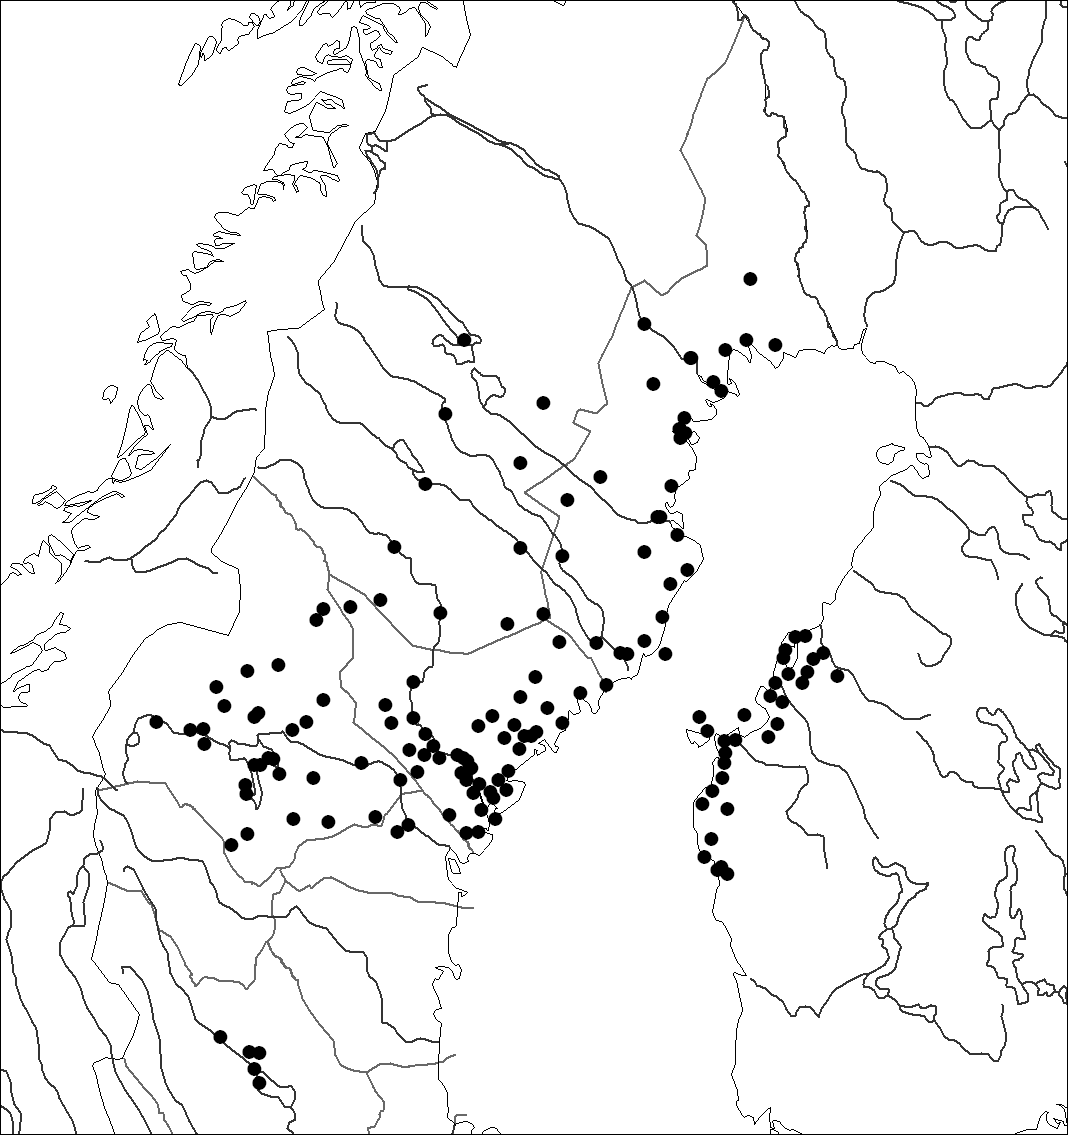
\includegraphics[height=.5\textheight]{figures/13_PresentDayDistribution}
\caption{Present-day distribution of non-delimited uses of definite nouns.}
\label{map:11}

\end{figure}

\subsection{ Areal distribution of non-delimited uses}

Although the map in \citet{Delsing2003a} shows non-delimited uses of definite nouns as being restricted to the Swedish-speaking areas of Norrbotten, Västerbotten, Österbotten, Ångermanland and parts of Jämtland, the distribution is in fact wider. In addition to the northern area just mentioned, non-delimited definites are quite strongly represented in the Ovansiljan area, and more or less sporadic examples are found also elsewhere in the Peripheral Swedish area. We shall first look at the two core areas.

\subsubsection{The northern core area}
It appears that non-delimited definites are normal in all Westrobothnian, Norrbothnian, Angermannian, and Ostrobothnian vernaculars, and the usage is fairly stable. It is striking that non-delimited definites are even found in the so-called “settler dialects” (\textstyleLinguisticExample{nybyggarmål}) of the province of Lappland, which are usually said to be strongly influenced by Standard Swedish. Compare the following example from Arvidsjaur in the south-western Lappland:

\ea %\label{} 
\langinfo{Arvidsjaur (Nm)}{}{}\\
\gll Jaa,  I  ska  berätt  för  je\\
yes  I  shall.{\prs}  tell.{\inf}  for  you\\
\gll då  ji  å  a  Karolina  nåppe  \textbf{snottren} i  höst.\\
when  I  and  {\pda}.{\f}  Karolina  pick.{\pst}  \textbf{cloudberries.{\deff}.{\pl}} in  autumn\\
\glt ‘Well, I’ll tell you how Karolina and I picked cloudberries last autumn.’\textsuperscript{ }[S4]

\z

In my opinion, Jämtland should also be included in the northern core area. Delsing is a bit vague here: he first mentions examples of definite forms after quantifiers from the Indal river valley, and then says that “partitive articles” (apparently in general) are “more frequent there than around Lake Storsjön and westward” (\citealt[19]{Delsing2003a}). On the map, he draws the western border of the use of the partitive article in non-delimited uses at the parish of Lit – this seems to be based on the distribution of quantified uses. However, it is fairly clear that non-delimited uses can be found all over the province (Bo Oscarsson, personal communication). The following is an example from the parish of Kall in the western part of Jämtland (the informant was born around 1850, the text was written down in 1908):

\ea %\label{} 
\langinfo{Kall (Jm)}{}{}\\
\gll En  vakker  ‘n  dag  rest  ‘n  åt  skoga\\
one  beautiful  {\pia}  day  go.{\pst}  he  to  forest.{\deff}\\
\gll å  skull  skaff  \textbf{ven}.\\
and  will.{\pst}  get.{\inf}  \textbf{wood.{\deff}}\\
\glt ‘One day he went to the forest to get firewood.’ [S11]

\z

\textbf{The southern core area (Ovansiljan)}. This area is much smaller than the northern one, and the strength of non-delimited uses is also more variable, suggesting a general receding tendency. The most stable usage is found in the more conservative vernaculars of Älvdalen, Våmhus, and Orsa. \citet[95]{Levander1909} quotes the following examples:

\ea%\label{}
\langinfo{Älvdalen (Os)}{}{}\\
\gll Ulum  fǫ  \textbf{stjyreð} et  middags.  \\
shall.{\prs}.1{\pl}  have.{\inf}  \textbf{curdled\_milk.{\deff}} to  dinner.{\gen}\footnotemark{} \\
\glt ‘We’ll have curdled milk for dinner.’

\z
\footnotetext{ This is a fossilized “old” genitive, see \sectref{sec:5.4.2}.} 
\ea
\gll Will  du  fǫ  \textbf{snuseð} min  mig?\\
want.{\prs}  you  have.{\inf}  \textbf{snuff.{\deff}} with  PRO.1{\sg}.{\obl}\\
\glt  ‘Do you want to have snuff from me?’

\z

More recent attestations can be quoted from Bengt Åkerberg’s translation of the novel \textstyleLinguisticExample{Hunden} by Kerstin Ekman:

\ea%\label{}
\langinfo{\label{bkm:Ref113183734}Älvdalen (Os) }{}{}\\
	\ea { 
		\gll 	Eð  liep  nið  \textbf{smeltwattneð} i  uäl\k{u}.  \\
				it  run.{\pst}  down  \textbf{melting\_water.{\deff}} in  hole.{\deff}.{\acc}  \\
		\glt 	‘Melting water was running down into the hole.’ [S9]
	}
	\ex {
	\gll 	Måyre;  war  ikåv  min  \textbf{wattne;}.\\
			marsh.{\deff}  be.{\pst}  pregnant  with  \textbf{water.{\deff}.{\dat}}\\
	\glt 	‘The marsh was pregnant with water.’ [S9]
	}
	\z
\z 
	
	(a) demonstrates the possibility of using a definite form in the dummy subject construction, showing that this is indeed possible also in the Ovansiljan area. 

Also in Mora, which has always been the centre of the Ovansiljan region, non-delimited uses of definite forms are relatively strong. Thus, the translation of \REF{30} in the Mormål version in the Cat Corpus is:

\ea %\label{} 
\langinfo{Mora (Os)}{}{}\\
\gll Ja,  bar  I  a  feir-in  wiråbördu,\\
yes  only  I  have.{\prs}  get\_in.{\supp}  wood\_bundle.{\deff}\\
\gll så  ska  I  werm  \textbf{mjotse} a  onum.\\
so  shall.{\prs}  I  warm.{\inf}  \textbf{milk.{\deff}} for  PRO.3{\sg}.{\m}.{\dat}\\
\glt ‘As soon as I have got the wood bundle into the house, I’ll warm some milk for him.’ (Cat Corpus)

\z

An example from the Bible texts in [S20]\textstyleLinguisticExample{:}

\ea %\label{} 
\langinfo{\label{bkm:Ref123968060}\textit{Östnors-seljamål} (Os)}{}{}\\
\gll Finns  ä  nån  …  såm  djäv  dem\\
exist.{\prs}  it  somebody    that  give.{\prs}  3{\pl}.{\obl}\\
\gll jen  wårm  när  dem  fråg  ettär  \textbf{fistjen?}\\
{\indf}  snake  when  they  ask.{\prs}  after  \textbf{fish.{\deff}}\\
\glt ‘Is there anybody … who gives them a snake when they ask for fish?’ (Matt. 7:10) [S20]

\z

In an older text we find the following:

\ea %\label{} 
\langinfo{\label{bkm:Ref123968062}Mora (Os)}{}{}\\
\gll Ä  wa  je  keLing  frammä,  so  add  selt  \textbf{brendunä}.\\
there  be.{\pst}  {\indf}  woman  out\_there  {\rel}  have.{\pst}  sell.{\supp}  \textbf{aquavit.{\deff}}\\
\glt ‘There was a woman out there, who had sold aquavit.’ [S46]

\z

(It may be noted that both \REF{47} and \REF{48} contain dummy subjects.)

However, the use of definite forms may be receding in Mormål. Compare the following parallel examples from the Elfdalian translation of the Gospel of John (\textstyleLinguisticExample{Juanneswaundsjila;}) and \textstyleLinguisticExample{Mormålsbibeln}:

\ea 
	\ea{ %\label{}
	\langinfo{Älvdalen (Os)}{}{}\\
	\gll 	Ed  so  ar  kumid  til  åv  tjyöt\k{i},  ed  ir  \textbf{tjyöted…}\\
			it  {\rel}  have.{\prs}  come.{\supp}  to  of  flesh.{\deff}.{\dat}  it  be.{\prs}  \textbf{flesh.{\deff}}\\
	\glt 	‘That which is born of flesh is flesh...’ (John 3:6) [S37]
	}
	\ex {
	\langinfo{\emph{Önamål} (Mora, Os)}{}{}\\
	\gll 	Er  så  a  kem-ti\textbf{l} åv  \textbf{tjöt} \textbf{  e} \textbf{  tjöt…}\\
			it  {\rel}  have.{\prs}  come\_about.{\supp}  of  \textbf{flesh} be.{\prs}  \textbf{flesh}\\
			
	\glt ‘That which is born of flesh is flesh...’\textbf{ }[S20]\textbf{ }
	}
	\ex {
	\langinfo{Älvdalen (Os)}{}{}\\
	\gll 	…ig  ar  kumid  og  döper  min  \textbf{wattne;}.\\
			I  have.{\prs}  come.{\supp}  and  baptize.{\prs}  with  \textbf{water.{\deff}.{\dat}}\\
	\glt 	‘…I have come to baptize with water.’ [S37]
	}
	\ex {
	\langinfo{\textit{Önamål} (Mora, Os)}{}{}\\
	\gll	…ar  I  kem  å  döpär  min  \textbf{wattn}.\\
			have.{\prs}  I  come.{\supp}  and  baptize.{\prs}  with  \textbf{water}\\
			
	\glt	‘…I have come to baptize with water.’ [S20]
	}
	\z 
\z

Among the other parishes in Ovansiljan, non-delimited definites are used fairly systematically in the Cat Corpus texts from Orsa and Våmhus: 

\ea 
	\ea {
	\langinfo{Orsa (Os)}{}{}\\
	\gll 	Ja,  bara  i  a  fendji  in  widn\\
			yes  only  I  have.{\prs}  get.{\supp}  in  firewood.{\deff}\\
	\gll 	så  skari  wärm  \textbf{mjötje} a  num.\\
			so  shall.{\prs}\_I  warm.{\inf}  \textbf{milk.{\deff}} for  PRO.3{\sg}.{\m}.{\dat}\\
	}
	\ex {
	\langinfo{Våmhus (Os)}{}{}\\
	\gll 	Ja,  bara  i  a  faið  in  wi:ðn,  \\
			yes  only  I  have.{\prs}  get.{\supp}  in  firewood.{\deff}  \\
	\gll 	so  ska  i  werm  \textbf{miö:ts\={i}} a  na.\\
			so  shall.{\prs}  I  warm.{\inf}  \textbf{milk.{\deff}} for  PRO.3{\sg}.{\f}.{\dat}\\
	\glt  	‘As soon as I have got the wood bundle into the house, I’ll warm some milk for him.’ (Cat Corpus)
	}
	\z 
\z

Similarly, in the extensive questionnaire materials from Orsa collected by Eva Olander, the overwhelming majority of the informants used definite forms in examples such as the following:

\ea %\label{} 
\langinfo{Orsa (Os)}{}{}\\
\gll An  drick  \textbf{mjötji}.\\
he  drink.{\prs}  \textbf{milk.{\deff}}\\
\glt ‘He drinks milk.’

\z

In Sollerön, the use of non-delimited definites appears to be weaker. Thus, according to informants, it would be most natural to use an indefinite form in the following example:

\ea %\label{} 
\langinfo{Sollerön (Os) }{}{}\\
\gll An  drikk  \textbf{mjok}.\\
he  drink.{\prs}  \textbf{milk}\\
\glt ‘He is drinking milk.’ (questionnaire)

\z

However, according to Margit Andersson (personal communication), it might be possible to use the definite form if a habitual interpretation is intended:

\ea %\label{} 
\langinfo{\label{bkm:Ref173318047}Sollerön (Os) }{}{}\\
\gll An  drikk  \textbf{mjotji}.\\
he  drink.{\prs}  \textbf{milk.{\deff}}\\
\glt ‘He drinks milk.’ 

\z

Similarly, \citet{AnderssonEtAl1999} quote examples such as the following, with bare nouns where e.g. Elfdalian, for example, would clearly use definite forms:

\ea%\label{}
\langinfo{Sollerön (Os) }{}{}\\
\gll I  åt  \textbf{bermos} ata  mjotjän.\\
I  eat.{\pst}  \textbf{lingonberry\_jam} with  milk.{\deff}.{\dat}\\
\glt ‘I ate lingonberry jam with the milk.’ (\citealt[373]{AnderssonEtAl1999})

\z

\ea
\gll Ä  e  \textbf{mjok} i  putällim.\\
it  be.{\prs}  \textbf{milk.{\deff}} in  bottle.{\deff}.{\dat}\\
\glt ‘There is milk in the bottle.’ (\citealt[373]{AnderssonEtAl1999})

\z

However, the same book also lists expressions such as \textstyleLinguisticExample{res päroni} ‘peel potatoes.{\deff}.{\pl}’ (\citealt[176]{AnderssonEtAl1999}). In the Cat Corpus, there is at least one clear case of a definite form:

\ea %\label{} 
\langinfo{Sollerön (Os) }{}{}\\
\gll …  å  ä  add  vurti  \textbf{skårån} upå  snjom.\\
  and  it  have.{\pst}  become.{\supp}  \textbf{hard\_crust.{\deff}} on  snow.{\deff}\\
\glt ‘… and there was a hard crust on the snow.’ (Cat Corpus)

\z

In the translation from Ore, which is regarded as a transitional variety between Ovansiljan and Nedansiljan, we find an indefinite form even in this sentence:

\ea %\label{} 
\langinfo{Ore (Os)}{}{}\\
\gll …  ô  ä  add  wurte  \textbf{skare} på  snjon.\\
  and  it  have.{\pst}  become.{\supp}  \textbf{hard\_crust} on  snow.{\deff}\\
\glt ‘… and there was a hard crust on the snow.’ (Cat Corpus)

\z

\subsubsection{Attestations outside the core areas}
 The areas where non-delimited uses are more sporadically represented include most of the rest of Norrland, and also the central province of Uppland, and possibly also Estonia. We shall look at each province in turn.

%\begin{styleBodytextheaded}
\subsubsection{Medelpad}
 This province is situated along the coast immediately south of Ångermanland. As in the case of Jämtland, \citet[19]{Delsing2003a} is a bit vague here. He quotes \citet[21]{Vestlund1923} as saying that an example such as \textit{de väks granen}\footnote{ “Vestlund (ibid.) nämner också att ångermanländska exempel med existentialkonstruktion, som hä väks granän [sic], är omöjliga i Medelpad.”}, registered in Häggdånger in southern Ångermanland and labeled an “existential construction” by Delsing, would be “completely impossible” in Medelpad. Somewhat later, Delsing says that for southern Norrland in general (and, as is clear from the map, including Medelpad) it seems that partitive articles have to be generic, which “among other things excludes existential constructions”. However, Vestlund has more to say on this issue in the work referred to by Delsing. In his comparison of Angermannian and Medelpadian, he says that in both vernaculars the definite form is used “to a considerably greater extent” than in the standard language\footnote{ “I såväl mp. som åm. användes best. form hos substantivet i betydligt större utsträckning än i riksspråket.” (\citealt[20]{Vestlund1923}) and that it is easy enough to hear expressions in Medelpad such as the following:

%\end{styleBodytextheaded}

\ea%\label{}
\langinfo{Selånger (Md)}{}{}\\
\gll nôppä  \textbf{bära}\\
pick.{\inf}  \textbf{berry.{\deff}.{\pl}}\\
\glt ‘pick berries’

\z

\ea
\gll sälä  \textbf{vön} \\
sell.{\inf}  \textbf{firewood.{\deff}} \\
\glt ‘sell firewood’

\z

\ea
\gll Vi  ha  fåt  \textbf{möN} ti  väjän.  \\
we  have.{\prs}  get.{\supp}  \textbf{ant.{\deff}} in  wall.{\deff}  \\
\glt ‘We have got ants in the wall.’

\z

\ea
\gll Hä  bli  \textbf{vakkär-värä} i  môra.\\
it  become.{\prs}  \textbf{nice\_weather.{\deff}} in  morning\\
\glt ‘The weather will be nice tomorrow.’

\z

Similarly, \citet[140]{Bogren1921} says that the vernacular of Torp, a parish in the western part of Medelpad, “uses the definite form in some phrases where the standard language has indefinite forms”.\footnote{ “Torpm. använder i en del fraser best. form där rspr har obest”} He gives additional examples such as:

\ea%\label{}
\langinfo{Torp (Md)}{}{}\\
\gll ha  \textbf{tin} \\
have.{\inf}  \textbf{time.{\deff}} \\
\glt ‘have time’

\z

\ea
\gll fara  \textbf{t} \textbf{8} \textbf{ge}\\
travel.{\inf}  \textbf{train.{\deff}}\\
\glt ‘go by train’

\z

It is therefore unclear what to make of Vestlund’s claim about the impossibility of sentences such as \textstyleLinguisticExample{de väks granen. }Curiously enough, it seems to be contradicted by the following example from one text that Vestlund himself edited, where there is a fairly clear case of a dummy subject construction:

%\begin{styleTextkrperErstzeileneinzugii}

%\end{styleTextkrperErstzeileneinzugii}

\ea%\label{}
\langinfo{Liden (Md)}{}{}\\
{}[Då han fick si bjO̍(r)n{}-dænn, sa vart-n sa ivri hætt han gLömde tell å slättje elen, å då han hadde sätt å(v) mæ bjOO̍(r)n, sa fek-n si hætt ]

\gll 	hæ  hôlle  på  brann  \textbf{skogelen}\\
		it  keep.PRET  on  burn.{\pst}  \textbf{forest\_fire.{\deff}}\\
\gll 	efrån  dær  han  hadde  lega,\\
		from  where  he   have.{\pst}  lie.{\supp}\\
\glt  	‘[When he saw that bear, he got so excited that he forgot to put out the fire, so he saw that] there was a forest fire burning where he had been lying.’ [S38]

\z

Admittedly, the text originates from Liden, the northernmost parish of Medelpad, and may not be representative of the province in general. 

\textbf{Hälsingland}. Going further south along the coast, we find that the vernaculars of Hälsingland do not in general seem to employ definite forms of nouns in non-delimited uses. Compare 

\ea %\label{} 
\langinfo{Färila (Hä)}{}{}\\
\gll De  hadde  vôrsste  \textbf{skâre} på  snön.\\
it  have.{\pst}  become.{\supp}  \textbf{crust} on  snow.{\deff}\\
\glt ‘There was a hard crust on the snow.’ (Cat Corpus)

\z

\ea %\label{} 
\langinfo{Järvsö (Hä)}{}{}\\
\gll Momma  va  på  väg  ut  ätte  \textbf{ve}.\\
Granny  be.{\pst}  on  way  out  after  \textbf{firewood}\\
\glt ‘Granny was on her way out to get firewood.’ (Cat Corpus)

\z

In a text originating from the parish of Bergsjö in the 1870’s, however, there are several examples that suggest that non-delimited uses were possible in earlier times in Hälsingland, e.g. the following (notice the dummy subject):

\ea%\label{}
\langinfo{\label{bkm:Ref154221800}Bergsjö (Hä)}{}{}\\
\gll Hæ  t$\omega $g  te  bɭåsæ  \textbf{sönnaväre}.\\
it  take.{\pst}  {{\inf}m}  blow.{\inf}  \textbf{southerly\_wind.{\deff}}\\
\glt ‘It started blowing from the south.’ [S28]

\z

\ea
\gll …o  jɷLə  $\Theta $pp  \textbf{elən} för  å  r$\Theta $sta  sə  en  kaffədr$\Theta $pa.\\
and  make.{\pst}  up  fire.{\deff}  for  {{\inf}m}  roast.{\inf}  {\refl}  {\indf}  coffee\_drop\\
\glt ‘…and made a fire to roast themselves a drop of coffee.’ [S28]

\z

We shall see that the use of a definite form of the noun ‘fire’ in lexical expressions such as ‘make a fire’ is particularly widespread.

\subsubsection{Härjedalen}
 Between the northern and southern core areas, we find the small province of Härjedalen, the vernaculars of which are traditionally regarded as “Norwegian”. \citet[28]{Reinhammar1973}, quoted by \citet[19]{Delsing2003a}, says rather cautiously that definite forms in general are “possibly less common” here than in other Norrlandic dialects. Delsing quotes some cases from Härjedalen texts where definite forms would be expected but do not occur. This is also in accordance with my findings, at least for non-delimited uses. Compare

\ea %\label{} 
\langinfo{Ljusnedal (Hd)}{}{}\\
\gll Dä  kommer  \textbf{snö} uppepå.\\
it  come.{\prs}  \textbf{snow} on\_top\\
\glt ‘There will be snow on top.’ (Cat Corpus)

\z

\subsubsection{Uppland}
Non-delimited uses of definites are in general not found in the vernaculars of the Mälar provinces. The only clear example mentioned in the literature is the following from Alunda in Uppland, in a transcription of the speech of a man born in 1880:

\ea %\label{} 
\langinfo{Alunda (Up)}{}{}\\ \label{bkm:Ref154222780}
 {}[Ann(â)rs sô brênde-råm åpp rörn ibʟann,] \\
\gll mênn  dôm  tord  (i)nt  sêttâ  \textbf{jêll’n} på  dê  \\
but  they  dare.{\pst}  {\neg}  put.{\inf}  \textbf{fire.{\deff}} on   that  \\
{} [för ê sjenâ åpp i skogen.]\\
\glt ‘[Otherwise they burnt the reeds sometimes,] but they did not dare to put fire to it, [since then it [the fire] would spread into the woods].’ (\citealt[60]{Västerlund1988}

\z

Here, we recognize the use of a definite form of the word for ‘fire’ in a lexicalized expression meaning ‘make fire’ or ‘put fire to’ that we also saw in \REF{63}(b) from Hälsingland. \citet[40]{Västerlund1988} comments that the use of the definite form of \textstyleLinguisticExample{jell} ‘fire’ is surprising in view of the fact that this “syntactic peculiarity”, i.e. an extended use of definite forms, “has earlier only been attested from Norrland, Dalarna and Värmland”.\footnote{ “…ägnat att förvåna, eftersom denna syntaktiska egenhet tidigare endast tycks vara känd från Norrland, Dalarna och Värmland.” (\citealt[60]{Västerlund1988}} I shall return to this kind of example below (\sectref{sec:3.2.3.1}).

\subsubsection{Nedersiljan}
 In the Nedersiljan vernaculars in Dalarna, non-delimited uses of definite forms do not in general seem possible, to judge from the written sources. Consider for instance the following example from Häradsbygden (Leksand):

\ea %\label{} 
\langinfo{Häradsbygden, Leksand (Ns) }{}{}\\
\gll Fôrst  skâ  o  körna,  gör  \textbf{ust} å  kok  \textbf{missmör}.\\
first  shall.{\prs}  she  churn.{\inf}  make.{\inf}  \textbf{cheese} and  cook.{\inf}  \textbf{whey-cheese}\\
\glt ‘First she’ll churn, make cheese and cook whey-cheese.’ [S48]

\z

%\begin{styleTextkrper}
However, in \citet{LevanderEtAl1961} I have found a couple of examples of what seems to be non-delimited uses:

%\end{styleTextkrper}

\ea %\label{} 
\langinfo{\label{bkm:Ref154222785}Leksand (Ns)}{}{}\\
\gll tännd  \textbf{jelln} ti  nävra\\
light.{\inf}  \textbf{fire.{\deff}} in  birch-bark\\
\glt ‘put fire to the birch-bark’

\z

\ea %\label{} 
\langinfo{Rättvik (Ns)}{}{}\\
\gll Vi  hallom-å  fåm  smått  om  \textbf{mjôltjä}.\\
we  {\prog}.{\prs}.1{\pl}  get.{\prs}.1{\pl}  little  about  \textbf{milk.{\deff}}\\
\glt ‘We’re getting short of milk.’

\z

%\begin{styleTextkrper}
These may be taken as suggesting that definite forms have been used earlier in these contexts.  Notice again the use of definite forms in the expression \textit{tännd jelln} ‘put fire to’.

%\end{styleTextkrper}

\subsubsection{Estonia}
 I have found a single plausible example of a non-delimited use of a definite form in an Estonian Swedish text. Interestingly, it comes from the very south-east end of the Swedish dialect area in the Baltics, from the small island of Runö (Estonian: Ruhnu) in the Bay of Riga, and is taken from \citet{Vendell1882}, thus representing a rather old variety. In the following example, there are several non-delimited nouns. Some of them are clearly indefinite, such as \textstyleLinguisticExample{brämin} ‘aquavit’ (definite form \textstyleLinguisticExample{brämini}); others could be both indefinite and definite, since the distinction is neutralized in plural forms, e.g. the plurale tantum \textstyleLinguisticExample{käta} ‘(the) meat’, but the word \textstyleLinguisticExample{kLimskin} appears to be an indisputable definite form (Vendell lists the base form of this word as \textstyleLinguisticExample{kLimsk}).

\ea%\label{}
\langinfo{\label{bkm:Ref136427219}Runö (Es)}{}{}\\
{}[Hesto ska bullupi kuma.] 

\gll 	Tua  ska  vi  dans,  ita  käta,\\
		then   shall.{\prs}  we  dance.{\inf}  eat.{\inf}  meat.{\pl}\\
\gll 	drikk  brämin,  \textbf{kLimskin,} ita  kLing  upa  hoitbre,\\
		drink.{\inf}  aquavit  \textbf{dumpling.{\deff}  } eat.{\inf}  butter  on  wheat bread\\
\gll 	kakubre,  setsurt  bre$\gamma $u,\\
		cake bread  sweet-sour  bread.{\pl}\\
\gll 	kouk  hurs  brufolki  kuma  uter  kirki.\\
		look.{\inf}  how  bride-people.{\deff}  come.{\prs}.{\pl}  out of   church.{\deff}\\
\glt 	‘[In autumn we’ll have the wedding.] Then we shall dance, eat meat, drink aquavit, (eat) dumplings,\footnote{ \textit{k}\textit{L}\textit{imsk} is used in the singular. It is somewhat unclear if it is a mass or a count noun – the corresponding Swedish word \textit{klimp} seems to be rather indifferent to the distinction.  } eat butter on wheat bread, cake bread, sweet-sour bread, watch how the newlyweds come out of church.’ (\citealt[76]{Vendell1882})

\z

\textbf{Norway}. \citet[16]{Delsing2003a} says that it is not clear to what extent “partitive articles” are used in Norway. “Some Norwegians associate the use with Trøndelag” [my transl.]. He quotes Iversen as “giving a few examples”; the ones he seems to have in mind (quoted above) are clearly generic, however. He says that he has found a few examples in texts that resemble North Swedish “partitive articles”, but mentions only one perhaps not too convincing example: 

\ea %\label{} 
\langinfo{Ytre Vikna (Nord-Trøndelag, Norway)}{}{}\\
\gll …der  vi  låog  å  drog  \textbf{garna.}\textit{  }\\
…where  we  lay.{\pst}   and  pull.{\pst}  \textbf{net.{\pl}.{\deff}} \\
\glt ‘…where we were pulling the fishing-nets.’ (\citealt[16]{Delsing2003a})

\z

Several Norwegian linguists whom I have asked have denied any knowledge of non-delimited uses of definites in Norwegian. 

\subsection{ Attestations of non-delimited uses from earlier periods}
\label{sec:3.2.3.1}

Probably the oldest attested example of a non-delimited use of a definite form from the Dalecarlian area, although not a particularly clear one, is in the oldest known wedding poem in a Swedish dialect, written in 1646 by a student at the university of Dorpat (present-day Tartu, Estonia, at the time one of the two universities on Swedish territory), who originated from Mora. The text is quoted in \citet[166]{Björklund1994}. The passage contains many obscure terms and rather than trying to translate it into English I quote it in the Appendix together with Björklund’s incomplete translation into Swedish. It consists of an enumeration of different kinds of food. Most of them are denoted by bare nouns, with one exception, \textstyleLinguisticExample{lunssfiskren, }translated by Björklund as \textstyleLinguisticExample{surfisk(en)} ‘(the) sour fish’, supposedly referring to fish preserved by salting. This is apparently a definite form, although the ending \textit{{}-ren} is unexpected (the definite form of \textit{fisk} ‘fish’ is \textit{fistjen} in the modern vernacular, cf. ex. \REF{47}). Such inconsistent usage of definite forms is common in older sources, and might be taken as an indication that the use of the definite form was optional, but it may also be interpreted as an influence from the standard language, or to the extent that the examples are from poetry, as a result of exigencies of the bound form. 

From the 18\textsuperscript{th} century, there are several clear examples, such as the following from 1716:

\ea %\label{} 
\langinfo{Dalecarlian (18\textsuperscript{th} century)}{}{}\\
\gll Färdas  um  näter,  og  \textbf{tobaken} räkia,\\
travel.{\inf}  about  night.{\pl}  and  \textbf{tobacco.{\deff}} smoke.{\inf}\\
\gll og  såfwå  å  marcki.\\
and  sleep.{\inf}  on   ground.{\deff}.{\dat}\\
\glt ‘Travel by night, smoke tobacco, and sleep on the ground’ [S25] 

\z

A similar example is found in \citet{Näsman1733}. It contains a definite form \textstyleLinguisticExample{Snustobakin} ‘snuff-tobacco.{\deff}’ which corresponds to an indefinite form in the accompanying Swedish translation (b), making the intended interpretation fairly clear:

\ea%\label{}
	\ea { 
	\langinfo{Mora (Os) (1733)}{}{}\\
	{}[Dug ir jen mann dug Ilof, soss satt mig i stukkin,]\\
	\gll	fær  ig  soup  \textbf{Snustobakin}\\
			for  I  inhale.{\pst}  \textbf{snuff-tobacco.{\deff}}\\
	\gll 	mæss  Præstn  hiælt  â  pridikâ.\\
			when  clergyman.{\deff}  keep.{\pst}  on   preach.{\inf}\\
	}
	\ex { \label{bkm:Ref139171019}Swedish1733
	\langinfo{Swedish (1733)}{}{}\\
	{}[Du är en mann du Elof, som satt mig i stocken,]\\
	\gll 	för  jag  söp  \textbf{Snustobak}\\
			for  I  inhale.{\pst}  \textbf{snuff-tobacco}\\
	\gll 	medan  Præstn  hölt  pâ  at  predika.\\
			while  clergyman.{\deff}  keep.{\pst}  on   {{\inf}m}  preach.{\inf}\\
			
	\glt  ‘[You’re some man you Elof, who put me in the stocks], because I was using snuff tobacco when the vicar was preaching.’
	}
	\z	
\z

From the northern area, the oldest attested example is from an 18\textsuperscript{th} century wedding poem from Nederluleå in the \textit{Lulemål} area in Norrbotten, which contains the following passage with several definite forms mixed with indefinite ones:

\ea %\label{} 
\langinfo{Nederluleå (Ll)}{}{}\\
{}[Gud hån bewåra dåm wel fra ou-aro\\
Gifwi dåm Hwäite å Råg nou i laro]\\
\gll Drick  uti  tonnen\\
drink.{\imp}  in  barrels.{\deff}.{\pl}\\
\gll kjött/  \textbf{fläske}  å  \textbf{kökin}  /\\
meat  \textbf{pork.{\deff}} and  \textbf{cake.{\deff}.{\pl}} \\
\gll Neda  fra  gålfwen  å  åltt  up  dill  tökin\\
down  from  floor.{\deff}.{\dat}  and  all  up  to  ceiling.{\deff}.{\dat}\\
\gll \textbf{Kouen} å  \textbf{ouxan} å  \textbf{gjeitren} å  \textbf{faara} \\
\textbf{cow.{\deff}.{\pl}} and  \textbf{ox.{\deff}.{\pl}} and  \textbf{goat.{\deff}.{\pl}} and  \textbf{sheep.{\deff}.{\pl}} \\
\glt ‘[God may save them from the bad years\\
Give them wheat and rye enough in the cases]\\
Drink in the barrels, meat, pork and cakes,\\
All the way from the floor to the ceiling\\
Cows and oxen and goats and sheep’ [S10]

\z

From the same time and area we also find multiple attestations of extended uses of definite forms in the word lists from \textit{Pitemål} compiled by the 18\textsuperscript{th} century Swedish philologist Johan Ihre, e.g. the typical expression \textstyleLinguisticExample{nåpp bera }‘to pick berries’ (\citealt{Reinhammar2002}.

Non-delimited uses of definite forms are thus attested as early as the 17\textsuperscript{th} century for Dalarna and the 18\textsuperscript{th} century for Upper Norrland, that is, more or less as early as we can get using written sources emanating from these areas. 

Going further back, it is quite clear that non-delimited uses of definite forms are not characteristic of Written Medieval Swedish. On the other hand, it is possible to find a few indications of such uses. We saw that the use of a definite form of the noun \textstyleLinguisticExample{eld/jell} ‘fire’ seems to be, or have been, possible in an area which is rather much wider than the one where non-delimited definites are commonly found (exs. \REF{63}(b), \REF{65}, \REF{67} above). This inspired me to do a search for such examples in medieval texts. I thus excerpted all occurrences of the word \textstyleLinguisticExample{eld(h)} ‘fire’ in the Old Swedish corpus \textstyleLinguisticExample{Källtext}, focusing on the use of this word in more or less lexicalized collocations as the object of verbs such as \textstyleLinguisticExample{tända} ‘light up’ and \textstyleLinguisticExample{göra} ‘make’. In the majority of all cases, a bare noun was used, but there were a few examples of definite forms, such as \REF{74}:

\ea %\label{} 
\langinfo{\label{bkm:Ref64457141}Medieval Written Swedish}{}{}\\
\gll Misther  falken  klöffwana,\\
lose.{\prs}  falcon.{\deff}  claw.{\deff}.{\pl}\\
\gll tha  tak  paper  oc  tänth  \textbf{elden}  thär  j\\
then  take.{\imp}  paper  and  light.{\imp}  \textbf{fire.{\deff}} there   in\\
%\begin{styleBlockQuote}
[oc bren the thaana som klöffwen wil aff falla, oc smör sidhan äffther mädh honagh oc bint bombas thär wm j nyo dagha]

%\end{styleBlockQuote}

\glt ‘Should the falcon lose its claws, then take paper and make fire therein [and burn the toes from which the claw is falling off, and rub afterwards with honey and tie a bandage around it for nine days].’ [S7]

\z

The quoted text is a complete and independent section of the manuscript in which it occurs; the possibility of an anaphoric interpretation is precluded because there is no mention of fire earlier in the text that \textit{elden} ‘fire.{\deff}’ could refer back to. The manuscript, “Bondakonst” from around 1500, was written by Peder Månsson (Petrus Magni), who was the last Catholic bishop of Västerås and the translator or author of several books. According to the 16\textsuperscript{th} century chronicle of Peder Swart, Peder Månsson was born in the parish of Tillberga in Västmanland, fairly close to the border with Uppland; he would thus have been a speaker of an Upper Swedish variety. However, in her monograph on Peder Månsson’s language, \citet[51]{Nordling2001} rejects this claim as not being trustworthy; thus, unfortunately, it does not seem possible to locate Peder Månsson linguistically. (More examples of this type from Written Medieval Swedish are found in the Appendix.) 

\subsection{ Typological parallels}
\label{sec:3.2.3.2}

Although the extension of definite marking to non-delimited uses of noun phrases that we find in the Peripheral Swedish area is typologically rather uncommon, and the possibility is not discussed at all in recent works such as \citet{Himmelmann1997} and \citet{Lyons1999}, it is not unique. One language where a parallel use is found is Spoken Moroccan Arabic.\footnote{ I am indebted to my former student Rashid El-Maaroufi who first made me aware of the Moroccan facts. } Thus, \citet[235]{Caubet1983} quotes the following example:

\ea
\langinfo{Moroccan Arabic}{}{}\\
\gll K\=ain  \textbf{əl-h̬obz.} \\
there-is  \textbf{{\deff}-bread}\\
\glt ‘There is bread.’

\z

While the definite article in other modern Arabic vernaculars does have a comparatively wide range of uses, it is not in general used in non-delimited noun phrases (Elie Wardini, personal communication). A detailed investigation of the use of definite articles in Arabic varieties could shed further light on the evolution of articles in general.

\subsection{ Uses with quantifiers}
\label{sec:3.2.4}
\label{bkm:Ref114303795}

A defining criterion of non-delimited uses was said in \sectref{sec:3.2.2} to be the absence of any expression that indicates individuation or a measure. However, in a part of the geographical area where non-delimited uses of definites are found, definite forms can also be used after quantifying expressions such as numerals or words meaning ‘many’, ‘few’ and the like. \citet{Delsing2003a} quotes examples such as \REF{76}.

\ea %\label{} 
\langinfo{\label{bkm:Ref64458018}\label{bkm:Ref159664857}Överkalix (Kx) }{}{}\\
\gll mitsi  \textbf{fålke}\\
much  \textbf{people.{\deff}}\\
\glt ‘many people’ (\citealt[17]{Delsing2003a})

\z

He says that the use is well attested in Norrbotten, Västerbotten and Ångermanland, and is also found along the river valley of Indalsälven in Jämtland. However, Delsing does not distinguish between cases like \REF{76} and constructions where the quantifier and the noun are linked by a preposition, as in \REF{77}.

\ea %\label{} 
\langinfo{Ragunda (Jm)}{}{}\\
\gll gott  om  \textbf{fistjevattna} \\
plenty  about  \textbf{fishing-water.{\deff}} \\
\glt ‘plenty of fishing-water’ (\citealt[18]{Delsing2003a})

\z

It appears that in the latter construction, where the noun has a more independent syntactic status, definite forms tend to be used more widely. In what follows, I shall be looking mainly at constructions of the first type, where the quantifier is immediately followed by a noun. 

\subsubsection{Westrobothnian}
 In this dialect area, the patterns seem different for numerals and other quantifiers such as ‘much’ and ‘many’. \citet{BergholmEtAl1999} studied three parishes representing different parts of the Westrobothnian dialect area: Bjurholm (transitional Angermannian-Westrobothnian), Burträsk (northern Westrobothnian), and Sorsele (southern Westrobothnian in the province of Lapland). For quantifiers other than numerals, it was only in Sorsele that the use of definite forms after quantifiers was predominant, most consistently after ‘much’, ‘many’ and ‘not any’:

\ea%\label{}
\langinfo{Sorsele (SVb)}{}{}\\
\gll Heä  \textbf{mycke} \textbf{snön} dära  backen.\\
it\_be.{\prs}  \textbf{much} \textbf{snow.{\deff}} there\_on  hill.{\deff}\\
\glt ‘There is much snow on the hill.’ (\citealt[24]{BergholmEtAl1999})

\z

\ea
\gll Han  drack  \textbf{mycke} \textbf{öle}.\\
he  drink.{\pst}  \textbf{much} \textbf{beer.{\deff}}\\
\glt ‘He drank a lot of beer.’ (\citealt[24]{BergholmEtAl1999})

\z 

\ea
\gll Han  ha  int  \textbf{na} \textbf{peninga}.\\
he  have.{\prs}  {\neg}  \textbf{any} \textbf{money.{\pl}.{\deff}}\\
\glt ‘He hasn’t got any money.’ (\citealt[24]{BergholmEtAl1999})

\z

In Burträsk and Bjurholm, definite forms with these quantifiers were uncommon or even “exceptions”, according to \citet{BergholmEtAl1999}. Curiously, the pattern with numerals was almost the opposite – here the Sorsele informants showed considerable variation and only the older informants tended to use definite forms consistently:

\ea %\label{} 
\langinfo{Sorsele (SVb) }{}{}\\
\gll Han  ha  \textbf{tre} \textbf{brödr} \textbf{en}.\\
he  have.{\prs}  \textbf{three} \textbf{brother.{\deff}.{\pl}}\\
\glt ‘He has three brothers.’ (\citealt[24]{BergholmEtAl1999})

\z

In both Burträsk and Bjurholm, however, definite forms were used with numerals ‘2’ and ‘3’ by most informants:

\ea %\label{} 
\langinfo{Bjurholm (ÅV)}{}{}\\
\gll \bfseries Han  ha  tre  brören.\\
\bfseries He  have.{\prs}  three  brother.{\deff}.{\pl}\\
\glt ‘He has three brothers.’ (\citealt[24]{BergholmEtAl1999})

\z

A similar example is also reported from Vilhelmina (SVb) by \citet{WälchliEtAl1998}. In a questionnaire from Arvidsjaur, definite forms are given as the only alternative after \textit{mycke} ‘much’. 

According to \citet[282]{ÅgrenEtAl1954}, presenting examples from Åsele (Åm) and Vilhelmina (Åm), the definite plural form in Laplandic vernaculars has “often totally ousted”\footnote{ “I de svenska målen i Lappland har däremot den bestämda flertalsformen ofta totalt trängt ut den obestämda, t.o.m. efter räkneord…” (\citealt[282]{ÅgrenEtAl1954}).} the indefinite form “even after numerals”.  \citet[17]{Delsing2003a} also quotes examples from these locations as well as from Örträsk (ÅV). 

\subsubsection{Norrbothnian}
 In \textit{Pitemål}, judging from the examples given in \citet{Brännström1993} and \citet{BerglundEtAl1991}, plural quantifiers are followed by the dative (see below), but definite forms without case marking are possible with \textstyleLinguisticExample{mö{\textasciigrave}tje} ‘much’, both in the singular and the plural:

\ea%\label{}
\langinfo{\textit{Pitemål} (Pm)}{}{}\\
\gll Hä  var  \textbf{mö{\textasciigrave}tje} \textbf{  foLKe} krö´gom  ´en.\\
it  be.{\pst}  \textbf{much} \textbf{people.{\deff}} around  he.{\obl}\\
\glt ‘There were a lot of people around him.’ (\citealt[52]{Brännström1993}

\z

\ea
\gll E  fj\={ö}ƚomsómmarn  var  {}-e  \textbf{m\={ö}tje} \textbf{  dj\={ä}tinga}.\\
?  last\_summer.{\deff}  be.{\pst}  it  \textbf{much} \textbf{wasp.{\deff}.{\pl}}\\
\glt ‘Last summer there were a lot of wasps.’ (\citealt[93]{BerglundEtAl1991})

\z

In \textit{Lulemål}, the use of the definite form seems relatively consistent after \textstyleLinguisticExample{mitji} – there are more than 30 examples in \citet{Nyström1993}, all except one with the definite form. 

\ea %\label{} 
\langinfo{\textit{Lulemål }(Ll)}{}{}\\
\gll He  vär  so  \textbf{åomitji} \textbf{pojkan} \textbf{o} \textbf{fLikken}\\
it  be.{\pst}  so  \textbf{very\_much} \textbf{boy.{\deff}.{\pl}} \textbf{and} \textbf{girl.{\deff}.{\pl}}\\
\gll ini  gämeLstän  dil  häLjen.\\
i  old\_town.{\deff}  to  holiday.{\deff}\\
\glt ‘There were so terribly many boys and girls in the church town\footnote{ This refers to the “Gammelstad church town” (included in the \textsc{UNESCO} World Heritage List), comprising more than 400 cottages serving as an overnight stop for parishioners coming from far-away. See http://www.lulea.se/gammelstad/.} during the holiday.’

\z

Similarly, from the Cat Corpus:

\ea %\label{} 
\langinfo{\textit{Lulemål }(Ll) }{}{}\\
\gll O  åt  tordes  jö  g\textbf{ä}  fr\textbf{ä}m  ati  gå\textbf{l}an  heler,\\
and  {\neg}  dare.{\pst}  I  go.{\inf}  up  to  farm.{\deff}.{\pl}  either\\
\gll för  der  v\textbf{ä}r  so  \textbf{mitji} \textbf{  heondan}.\\
for  there  be.{\pst}  so  \textbf{much} \textbf{dog.{\deff}.{\pl}}\\
\glt ‘And I didn’t dare go close to the farms either, for there were so many dogs.’ (Cat Corpus)

\z

From Råneå in the \textit{Lulemål} area, \citet[17]{Delsing2003a} quotes\textbf{ }\textstyleLinguisticExample{mitsi bröde } ‘much bread.{\deff}’\textbf{. }

However, with most other quantifiers, including \textstyleLinguisticExample{meir} ‘more’, negative quantifiers such as \textstyleLinguisticExample{öyngar} ‘none’ and \textstyleLinguisticExample{ånt na} ‘not any’, and numerals, only indefinite forms show up:

\ea%\label{}
\langinfo{\textit{Lulemål} (Ll) }{}{}\\
\gll Ho  hä  \textbf{öynge} \textbf{förhål}.\\
she  have.{\prs}  \textbf{no} \textbf{restraint}\\
\glt ‘She has no restraint, i.e. she cannot restrain herself.’ (\citealt{Nyström1993}

\z

\ea
\gll Ini  skapen  f\textbf{ä}nnsch  e  bara  \textbf{tvo} \textbf{  kålper,}\\
in  cupboard.{\deff}  exist.{\pst}  it  only  \textbf{two} \textbf{cold\_potato}\\
\gll in  litn  korvbuyt  o  \textbf{in} \textbf{  hå} \textbf{l} \textbf{v} \textbf{  lök}.\\
One  small  sausage\_piece  and  \textbf{one} \textbf{half} \textbf{onion}\\
\glt ‘In the cupboard there were only two cold potatoes, one small piece of sausage and half an onion.’ (Cat Corpus)

\z

Delsing quotes the example \textstyleLinguisticExample{nå döfolke }from \textit{Lulemål}, with the intended interpretation ‘some dead people’. This would be the only such example from Norrbotten. However, since other sources give the form \textstyleLinguisticExample{nä} for ‘some’ in \textit{Lulemål}, which should according to \citet{Nordström1925} be followed by an indefinite form in the singular and a dative form in the plural, some checking of the source seems to be warranted. The texts Delsing refers to for \textit{Lulemål} do not as far as I can see contain any such phrase, but there is a passage in the text [S31] which might have been misinterpreted. It contains the phrase \textstyleLinguisticExample{spadd upa n}ɷ\textstyleLinguisticExample{ döfolke}, where the first three words are translated in a footnote as ‘put on him by evil magic’ [“trollade på honom”], where \textstyleLinguisticExample{n}ɷ is the dative form of ‘him’; ‘some dead people’ would rather be \textstyleLinguisticExample{nä döfolk}. 

From the Kalix area, we find examples both with ‘much’ and with numerals:

\ea%\label{}
\langinfo{Nederkalix (Kx) }{}{}\\
\gll \bfseries Wå  söynda  skå  dö  vä  så  myttji  sopan?\\
\bfseries What  sin.{\deff}  shall.{\prs}  you  with  so  much  milk.{\deff}\\
\glt ‘What the hell are you going to do with so \textbf{much milk}?’ (Cat Corpus)

\z

\ea
\gll \textbf{A} \textbf{tåo} \textbf{fram} \textbf{to} \textbf{\textit{  }} \textbf{kålpotåtisan} \textbf{\textit{,}}\\
\bfseries
she  take.{\pst}  out  two  cold\_potato.{\deff}.{\pl}\\
\gll in  kårvbäit  å  in  hålv  lök.\\
one  sausage-piece  and  one  half  onion\\
\glt ‘She took out two cold potatoes, a piece of sausage, and half an onion.’ (Cat Corpus)
\z

\exewidth{(123)}

\ea %\label{} 
\langinfo{Siknäs, Nederkalix (Kx)}{}{}\\
\gll så  forskrätseli  \textbf{mytji} \textbf{smöre}\\
so  terribly  \textbf{much} \textbf{butter.{\deff}}\\
\glt ‘so terribly much butter’ (\citealt{Stenberg1971}

\z

For Överkalix, cf. (76) above, with ‘much’. Definites with numerals are not attested from Överkalix, however.

\subsubsection{Northern Settler Area}
In a questionnaire from Arvidsjaur, definite forms are given as the only alternative after \textit{mycke} ‘much’, \textit{nå} ‘some’, and alternating with indefinites after numerals.

\subsubsection{Ostrobothnian}
 For Karleby, \citet[94]{Hagfors1891} quotes the examples \textstyleLinguisticExample{mytji järne} ‘much iron.{\deff}’ and \textstyleLinguisticExample{na lite tjöte} ‘some little meat.{\deff}’. For the same vernacular, as described by \citet{Vangsnes2003}, the use of definite forms is obligatory after \textstyleLinguisticExample{mytji} ‘much’ and \textstyleLinguisticExample{somt} ‘some, certain’:

\ea %\label{} 
\langinfo{Karleby (NOb)}{}{}\\
\gll mytji  öle\\
much  beer.{\deff}\\
\glt ‘much beer’

\z

This is only visible in the singular since the Karleby vernacular has neutralization of definiteness in the plural. To make things more complex, other quantifiers, such as \textstyleLinguisticExample{mang} ‘many’, \textstyleLinguisticExample{noga} ‘some’ and numerals, require the indefinite singular of the following noun (possibly under Finnish influence):

\ea %\label{} 
\langinfo{Karleby (NOb)}{}{}\\
\gll tri  hest\\
three  horse.{\sg}.{\indf}\\
\glt ‘three horses’

\z

\citet[26]{ErikssonEtAl1999}, in their questionnaire investigation of Ostrobothnian, report that, in general, their informants did not use definite forms after quantifiers. One exception was a person from Pedersöre, a neighbour parish of Karleby. Even this informant showed variation (e.g. \textstyleLinguisticExample{mytchi öli} ‘much beer.{\deff}’ but \textstyleLinguisticExample{mytchi snö} ‘much snow’.) Two informants from Malax in their material used a definite form after \textstyleLinguisticExample{itt na} ‘not any’ in the following example:

\ea %\label{} 
\langinfo{Malax (SOb)}{}{}\\
\gll He  je  itt  \textbf{na} \textbf{snön} på  martje.\\
it  be.{\prs}  {\neg}  \textbf{any} \textbf{snow.{\deff}} on  ground.{\deff}\\
\glt ‘There is not any snow on the ground.’ (questionnaire)

\z

It does seem that the use of definite forms after quantifiers in Österbotten is basically restricted to the northernmost part.

\subsubsection{Jämtland}
Delsing quotes three examples from written texts, but two of them are prepositional constructions, so the only remaining one would be \textstyleLinguisticExample{nå brännvine} ‘some vodka’ from Lit. I have not been able to find any other attestations from Jämtland.

\subsubsection{Ångermanland}
 Delsing reports four examples from written texts, two with \textstyleLinguisticExample{myttje} (Tåsjö, Anundsjö) and two with \textstyleLinguisticExample{na }(Säbrå, Stigsjö). \citet{WälchliEtAl1998} quote the following examples from Edsele:

\ea%\label{}
\langinfo{Edsele (Åm)}{}{}\\
\gll Där  vax  {}-e  \textbf{mötje} \textbf{  gräse}.\\
there  grow.{\pst}  it  \textbf{much} \textbf{grass.{\deff}}\\
\glt ‘There was much grass.’ [S5]

\z

\ea
\gll Män  hon  fann  \textbf{inge} \textbf{ägga}\\
but  she  find.{\pst}  \textbf{no.{\pl}} \textbf{egg.{\deff}.{\pl}}\\
\gll utan  sto  där  utan  ägg  o  utan  höne\\
but  stand.{\pst}  there  without  egg.{\pl}  and  without  hen\\
\glt ‘But she did not find any eggs but stood there without eggs and without a hen.’ [S5]

\z

In the Cat Corpus, we find the following examples:

\ea%\label{}
\langinfo{Junsele (Åm)}{}{}\\
\gll Momma  hadd  bodd  eschammen\\
Granny  have.{\pst}  live.{\supp}  alone\\
\gll häri  stugern  \textbf{mang} \textbf{  e} \textbf{  åra} nu.\\
in  hut.{\deff}  \textbf{many} \textbf{{\pia}} \textbf{year.{\deff}.{\pl}} now\\
\glt ‘Granny had lived alone in the cabin for many years now.’ (Cat Corpus)

\z

\ea
\gll Momma  titte  åt  sia,   steg  opp  å\\
Granny  look.{\pst}  at  side  rise.{\pst}  up  and\\
\gll geck  hit  tell  fönstre  å  gnôp  tå\\
go.{\pst}  here  to  window.{\deff}  and  pinch.{\pst}  off\\
\gll \textbf{na} \textbf{  gulblaa} tå  blomma  däri  fönstre.\\
\textbf{some} \textbf{yellow\_leave.{\deff}.{\pl}} from  flower.{\deff}  in  window.{\deff}\\
\glt ‘Granny looked aside, got up and went up to the window, and pinched off some yellow leaves from the plant in the window.’ (Cat Corpus)

\z

No examples with numerals are attested from this area, to my knowledge.

\subsubsection{Dalecarlian}
Definite forms are not in general used with quantifiers in any Dalecarlian variety. In the literature, counterinstances to this are found in two places, both from Älvdalen. One is discussed below under the heading “Earlier periods”, the other is a brief mention in \citet[95]{Levander1909}, where it is said that definite forms are “occasionally” found with \textstyleLinguisticExample{någär }‘some’, as in \textstyleLinguisticExample{nå grandeð }‘a little bit’ – which looks like a set expression, although it is hard to tell, since no details are given.

\subsubsection{Earlier periods}
 In Written Medieval Swedish, quantifiers and interrogative pronouns were sometimes followed by a definite noun. At least two different types can be distinguished (Wessén (1956: 36--37). One can be labeled “true partitive” – the noun refers to a specific superset, that is, a larger set from which a member or a subset is picked out by the quantifier or interrogative pronoun:

\ea%\label{}
\langinfo{Written Medieval Swedish}{}{}\\
\gll\bfseries
somlikin  sädhin\\
\bfseries
some  grain.{\deff}\\
\glt ‘some of the grain’

\z

\ea
\gll Han  sporde,  \textbf{hulkom} \textbf{gudhenom} thet  teknit  tilhörde.\\
he  ask.{\pst}  \textbf{which.{\dat}.{\sg}.{\m}} \textbf{god.{\deff}.{\dat}.{\sg}} that.{\n}  sign.{\deff}  belong.{\pst}\\
\glt ‘He asked which of the gods the sign belonged to.’ [S36]

\z

This type of definite, then, is different from what we find in quantifier phrases in modern vernaculars where there is no specific superset involved. The construction was probably a general feature of older forms of Scandinavian and survives in Modern Icelandic. The Icelandic use is mentioned by \citet{Riesler2002} as a typological parallel to the “partitive” uses of definite forms in northern Scandinavian, but there is no overlap between the two types. Although this fact does not exclude a diachronic relationship, there is to my knowledge no historical evidence to suggest such a connection.

The second medieval Swedish type at first seems more like the modern Peripheral Swedish area one. Compare:

\ea %\label{} 
\langinfo{\label{bkm:Ref78603361}Written Medieval Swedish}{}{}\\
\gll Tha  war  om siidher  \textbf{engin} \textbf{födhan} i  stadhenom.\\
then  be.{\pst}  finally  \textbf{no} \textbf{food.{\deff}} in  town.{\deff}.{\dat}\\
\glt ‘Eventually, there wasn’t any food in the town.’ [S32]

\z

However, it turns out that the distribution of definite forms after quantifiers is different in medieval Swedish than in the modern vernaculars. Wessén notes that the definite form is most common with the inherently negative \textstyleLinguisticExample{ängin} ‘no, none’. Among the rather numerous examples he lists, there are only two that contain another quantifier, and in one of these, the quantifier is clearly within the scope of a negation: 

\ea %\label{} 
\langinfo{Written Medieval Swedish}{}{}\\
\gll …medhan  the  orkadho\\
…while  they  be\_able\_to.{\pst}.3{\pl}\\
\gll ekke  bära  \textbf{mykin} \textbf{  matin} mz  sik.\\
{\neg}  carry.{\inf}  \textbf{much} \textbf{food.{\deff}} with  {\refl}\\
\glt  ‘…while they did not manage to carry much food.’ [S6]

\z

The only example that is neither inherently negative nor within the scope of a negation is the following:

\ea %\label{} 
\langinfo{\label{bkm:Ref78603365}Written Medieval Swedish}{}{}\\
\gll …æn  hans  discipuli  gingo  in  i  stadhin\\
…but  he.{\gen}  disciple.{\pl}  go.{\pst}  in  in  town.{\deff}\\
\gll at  faa  them  \textbf{nakan} \textbf{matin}.\\
to  get.{\inf}  them  \textbf{some.{\acc}.{\sg}.{\m}} \textbf{food.{\deff}}\\
\glt ‘… but his disciples went into the town to get some food.’ [S6]

\z

The pattern represented by \REF{93}--\REF{95} does not appear to have been a general one in Written Medieval Swedish. In the Källtext corpus, most occurrences of \textstyleLinguisticExample{ängin} ‘no, none’ are followed by indefinite nouns. Most of Wessén’s examples come from a few texts (the Pentateuch, Bonaventura), and even in those texts the pattern appears exceptional. On the other hand, the use still survived in some 16\textsuperscript{th} century texts, notably the New Testament translation of 1526:

\ea %\label{} 
\langinfo{Early Modern Swedish}{}{}\\
\gll Wij  haffuom  \textbf{intit} \textbf{brödith}.\\
we  have.{\prs}.1{\pl}  \textbf{no.{\n}} \textbf{bread.{\deff}}\\
\glt ‘We have no bread.’ [S30]

\z

There is an intriguing example from an early text in what purports to be Elfdalian (\citealt{Näsman1733}:

\ea %\label{} 
\langinfo{\label{bkm:Ref108604709}Älvdalen (Os) (18\textsuperscript{th} century)}{}{}\\
\gll \textbf{…ingan} \textbf{uidn} klufin…\\
\textbf{…no} \textbf{firewood.{\deff}} hew.{\pp}…\\
\glt ‘…no firewood hewn…’

\z

When Lars Levander transcribed this text in \citet[T117]{Lundell1936}, “normalizing” it according to early 20th century usage, he changed this phrase into \textstyleLinguisticExample{inggan wi kluvnan}.\footnote{ Or rather, using the Swedish dialect alphabet (landsmålsalfabetetet):  }\textit{ }It is impossible to tell whether \REF{97} really represents 18\textsuperscript{th} century Elfdalian or not. 

A fairly similar pattern is found in Norwegian, both the standard varieties and the dialects. The following sentence is quoted by \citet[302]{FaarlundEtAl1997} as one of several examples where “individual predicative expressions in negated sentences” take a definite suffix on the noun. 

\ea %\label{} 
\langinfo{Bokmål Norwegian }{}{}\\
\gll \textbf{Mange} \textbf{  kronene} var  det  ikke.\\
\textbf{many} \textbf{crown.{\pl}} be.{\pst}  it  {\neg}\\
\glt ‘Many crowns it wasn’t.’

\z

However, with quantifiers this pattern is not restricted to predicative positions. Examples like the following are quite common:\footnote{ A Google search for the string “tok ikke mange” yielded 1360 hits, and of the first 50 examples more than 80 per cent were followed by a definite noun.}

\ea%\label{}
\langinfo{Bokmål Norwegian }{}{}\\
\gll De  snakket  ikke   \textbf{mange} \textbf{  ordene}.\\ % {\href{http://kh.hd.uib.no/cgi-dos/roman-bm.bat?P55377C00#here}{ikke}}
		they  talk.{\pst}  {\neg}  \textbf{many} \textbf{word.{\pl}.{\deff}}\\
\glt ‘They didn’t speak many words.’ (Internet)

\z

\ea
\gll Det  tok  ikke  \textbf{mange} \textbf{sekundene}\\ %\href{http://kh.hd.uib.no/cgi-dos/roman-bm.bat?P18543500#here}
it  take.{\pst}  {\neg}  \textbf{many} \textbf{second.{\pl}.{\deff}}\\
\gll før  døren  var  åpen.\\
before  door.{\deff}  be.{\pst}  open\\
\glt  ‘It didn’t take many seconds before the door was open.’ (Internet)

\z

Compare also examples such as the following, in which a definite noun with indefinite meaning is used in the scope of negation:

\ea %\label{} 
\langinfo{Tromsø (Troms, Norway)}{}{}\\
\gll Han  eide  \textbf{ikkje} \textbf{nåla} i  væggen.\\
he  own.{\pst}  \textbf{{\neg}} \textbf{nail.{\deff}} in  wall.{\deff}\\
\glt ‘He did not own a nail (lit. the nail) in the wall.’ (\citealt[18]{Iversen1918})

\z

\subsubsection{Datives after quantifiers}
This is a topic that I have treated in another paper (\citealt{Dahl2008}, and although it is related to the question of definite marking, it is strictly speaking separate from it, so I will only briefly state the facts here. In the dialect areas Northern Westrobothnian, \textit{Pitemål} and \textit{Lulemål}\footnote{ As I was later informed by Oskar Rönnberg, the phenomena described here for \textit{Pitemål} and \textit{Lulemål} are also found in \textit{Kalixmål}\textit{ }as spoken in Kalix.}, a quantifier may be followed by a form which is diachronically (and at least in some varieties also synchronically) a definite dative plural form. In \textit{Pitemål} and \textit{Lulemål}, this is obligatory after \textit{na} ‘some’:

\ea %\label{} 
\langinfo{\textit{Pitemål }(Pm)}{}{}\\
\gll Hä  kom  \textbf{na} \textbf{  fLi{\textasciigrave}ttjom} ötät  väjen.\\
it  come.{\pst}  \textbf{some} \textbf{girl.{\dat}.{\pl}} along  road.{\deff}\\
\glt ‘There came some girls along the road.’ (\citealt[19]{Brännström1993} 

\z

In a curious development restricted to the southern Norrbothnian varieties –  \textit{Pitemål} and \textit{Lulemål} – this pattern has spread in such a way that the erstwhile dative plural form is also used in contexts where there is no quantifier, notably when some modifier such as an adjective or a possessive pronoun precedes the noun. Examples from Råneå (Lm) are \textstyleLinguisticExample{truy swårta faro} ‘three black sheep’, \textstyleLinguisticExample{våder bano å dåmers aongo} ‘our children and their [other people’s] brats’, \textstyleLinguisticExample{nuya kLedo} ‘new clothes’ (Råneå (\citealt{Wikberg2004}. An unexpected property of these constructions is that they contain a non-apocopated form of the plural adjectives, with the weak ending\textit{ {}-a }(\citet[36]{Dahlstedt1956}. In fact, such combinations of non-apocopated adjectives and dative-marked nouns are in competition with the construction that would be expected in such contexts, viz. definite nouns with incorporated adjectives. Compare the following examples which illustrate the two possibilities:

\ea%\label{}
\langinfo{\textit{Lulemål} (Lm)}{}{}\\
\gll Hån  hä  fo  fLugo,\\
he  have.{\prs}  get.{\supp}  fly\\
\gll hån  hä  låga  se  \textbf{wita} \textbf{bökso}\\
he  have.{\prs}  make.{\deff}  {\refl}  \textbf{white} \textbf{trouser.{\dat}.{\pl}}\\
\glt ‘He’s got crazy, he has got himself white trousers.’

\z

\ea
\gll Hån  kåm  o  lovere  ini  \textbf{witböxen}.\\
he  come.{\pst}  and  brag.{\pst}  in  \textbf{white\_trouser.{\deff}.{\dat}.{\pl}}\\
\glt ‘He came bragging in white trousers.’ (\citealt[105]{Nyström1993}

\z

In \citet{Dahl2008}, I suggest as a possible scenario that the construction with an adjective in\textit{ {}-a} and a noun in the historical dative form has arisen as an attempt to fill what seemed like a gap in the paradigm, namely an analogue to Swedish premodified indefinite noun phrase. It should be noted in this context that the original indefinite plurals in these vernaculars have by and large lost their endings while retaining the grave pitch accent, at the same time as they have become restricted in their use to combinations with numerals. The following example illustrates how such endingless forms alternate with historical dative forms: 

\ea %\label{} 
\langinfo{\textit{Pitemål} (Pm)}{}{}\\
\gll Hä  stå:r  \textbf{\`{å}ått} \textbf{àasp} d\=ena  b\`{å}årt,\\
it  stand.{\prs}  \textbf{eight} \textbf{aspen.{\pl}} there  away\\
\gll å  hä  jär  \textbf{sto:ra} \textbf{àspom}.\\
and  it  be.{\prs}  \textbf{big.{\pl}} \textbf{aspen.{\dat}.{\pl}}\\
\glt ‘There are eight aspens over there, and they are big aspens.’ (\citealt[20]{BerglundEtAl1991})

\z

Such plural forms are used also in premodified noun phrases. Thus, according to the suggested scenario, the\textit{ {}-a} ending was directly imported from Swedish, while the original dative forms in\textit{ {}-om/-o,} which were used with quantifiers such as \textit{na},\textit{ }were apparently seen as more natural alternatives to Swedish plural nouns than the endingless historical indefinites. Some nouns, however, retain plural forms that are also distinct from the singular forms at the segmental level, e.g. \textit{Pitemål} \textit{ha´nd: hénder} ‘hand:hand.{\pl}’.  Such plural forms are also used in pre-modified noun phrases rather than the historical datives, the reason presumably being that these forms were more directly analogous to Swedish plurals than the endingless ones. 

\subsubsection{Definites after quantifiers: Summing up}
The use of definite forms after quantifiers in the Swedish dialect area is more restricted than the non-delimited use. The dialectal areas involved are Norrbothnian, the Northern Settler Area, Westrobothnian, Jämtland, Angermannian, and Ostrobothnian, that is, in principle corresponding to the whole northern “core area” of non-delimited uses, while the southern “core area” (Ovansiljan) lacks attestations except for the marginal examples from Älvdalen. But even within the northern area, there is considerable variation. What is most striking is that the geographical distribution of the attestations differs quite considerably between the various quantifiers involved, as can be seen in \figref{map:12}--\figref{map:15}. Since attestations tend to be somewhat sporadic, one should be somewhat cautious with conclusions, but there seem to be some fairly clear tendencies. Thus, the use of definite forms after numerals is almost exclusively attested in the county (not the province!) of Västerbotten – which is not an entity according to the dialectological tradition, but rather consists of parts of four different dialect areas in Dahlstedt’s maps. The use of dative after quantifiers is also a geographically restricted phenomenon, found in Northern Westrobothnian, \textit{Pitemål} and \textit{Lulemål}. 

The historical relationships between the uses of definite nouns after quantifiers in Scandinavian are not clear. Disregarding the true partitive uses, the definite forms in older Swedish, Norwegian, and the singular example from 18\textsuperscript{th} century Dalecarlian, seem to be “negative polarity items”, that is, they occur basically only within the scope of negation (with \REF{95} as the only attested exception). In the Peripheral Swedish vernaculars where definite nouns show up after quantifiers, there is no such limitation – on the contrary, in some varieties the definite forms are used primarily with ‘much’. I would therefore submit that we are dealing with two separate developments. 

\begin{figure}[h]

%\begin{styleBeschriftung}
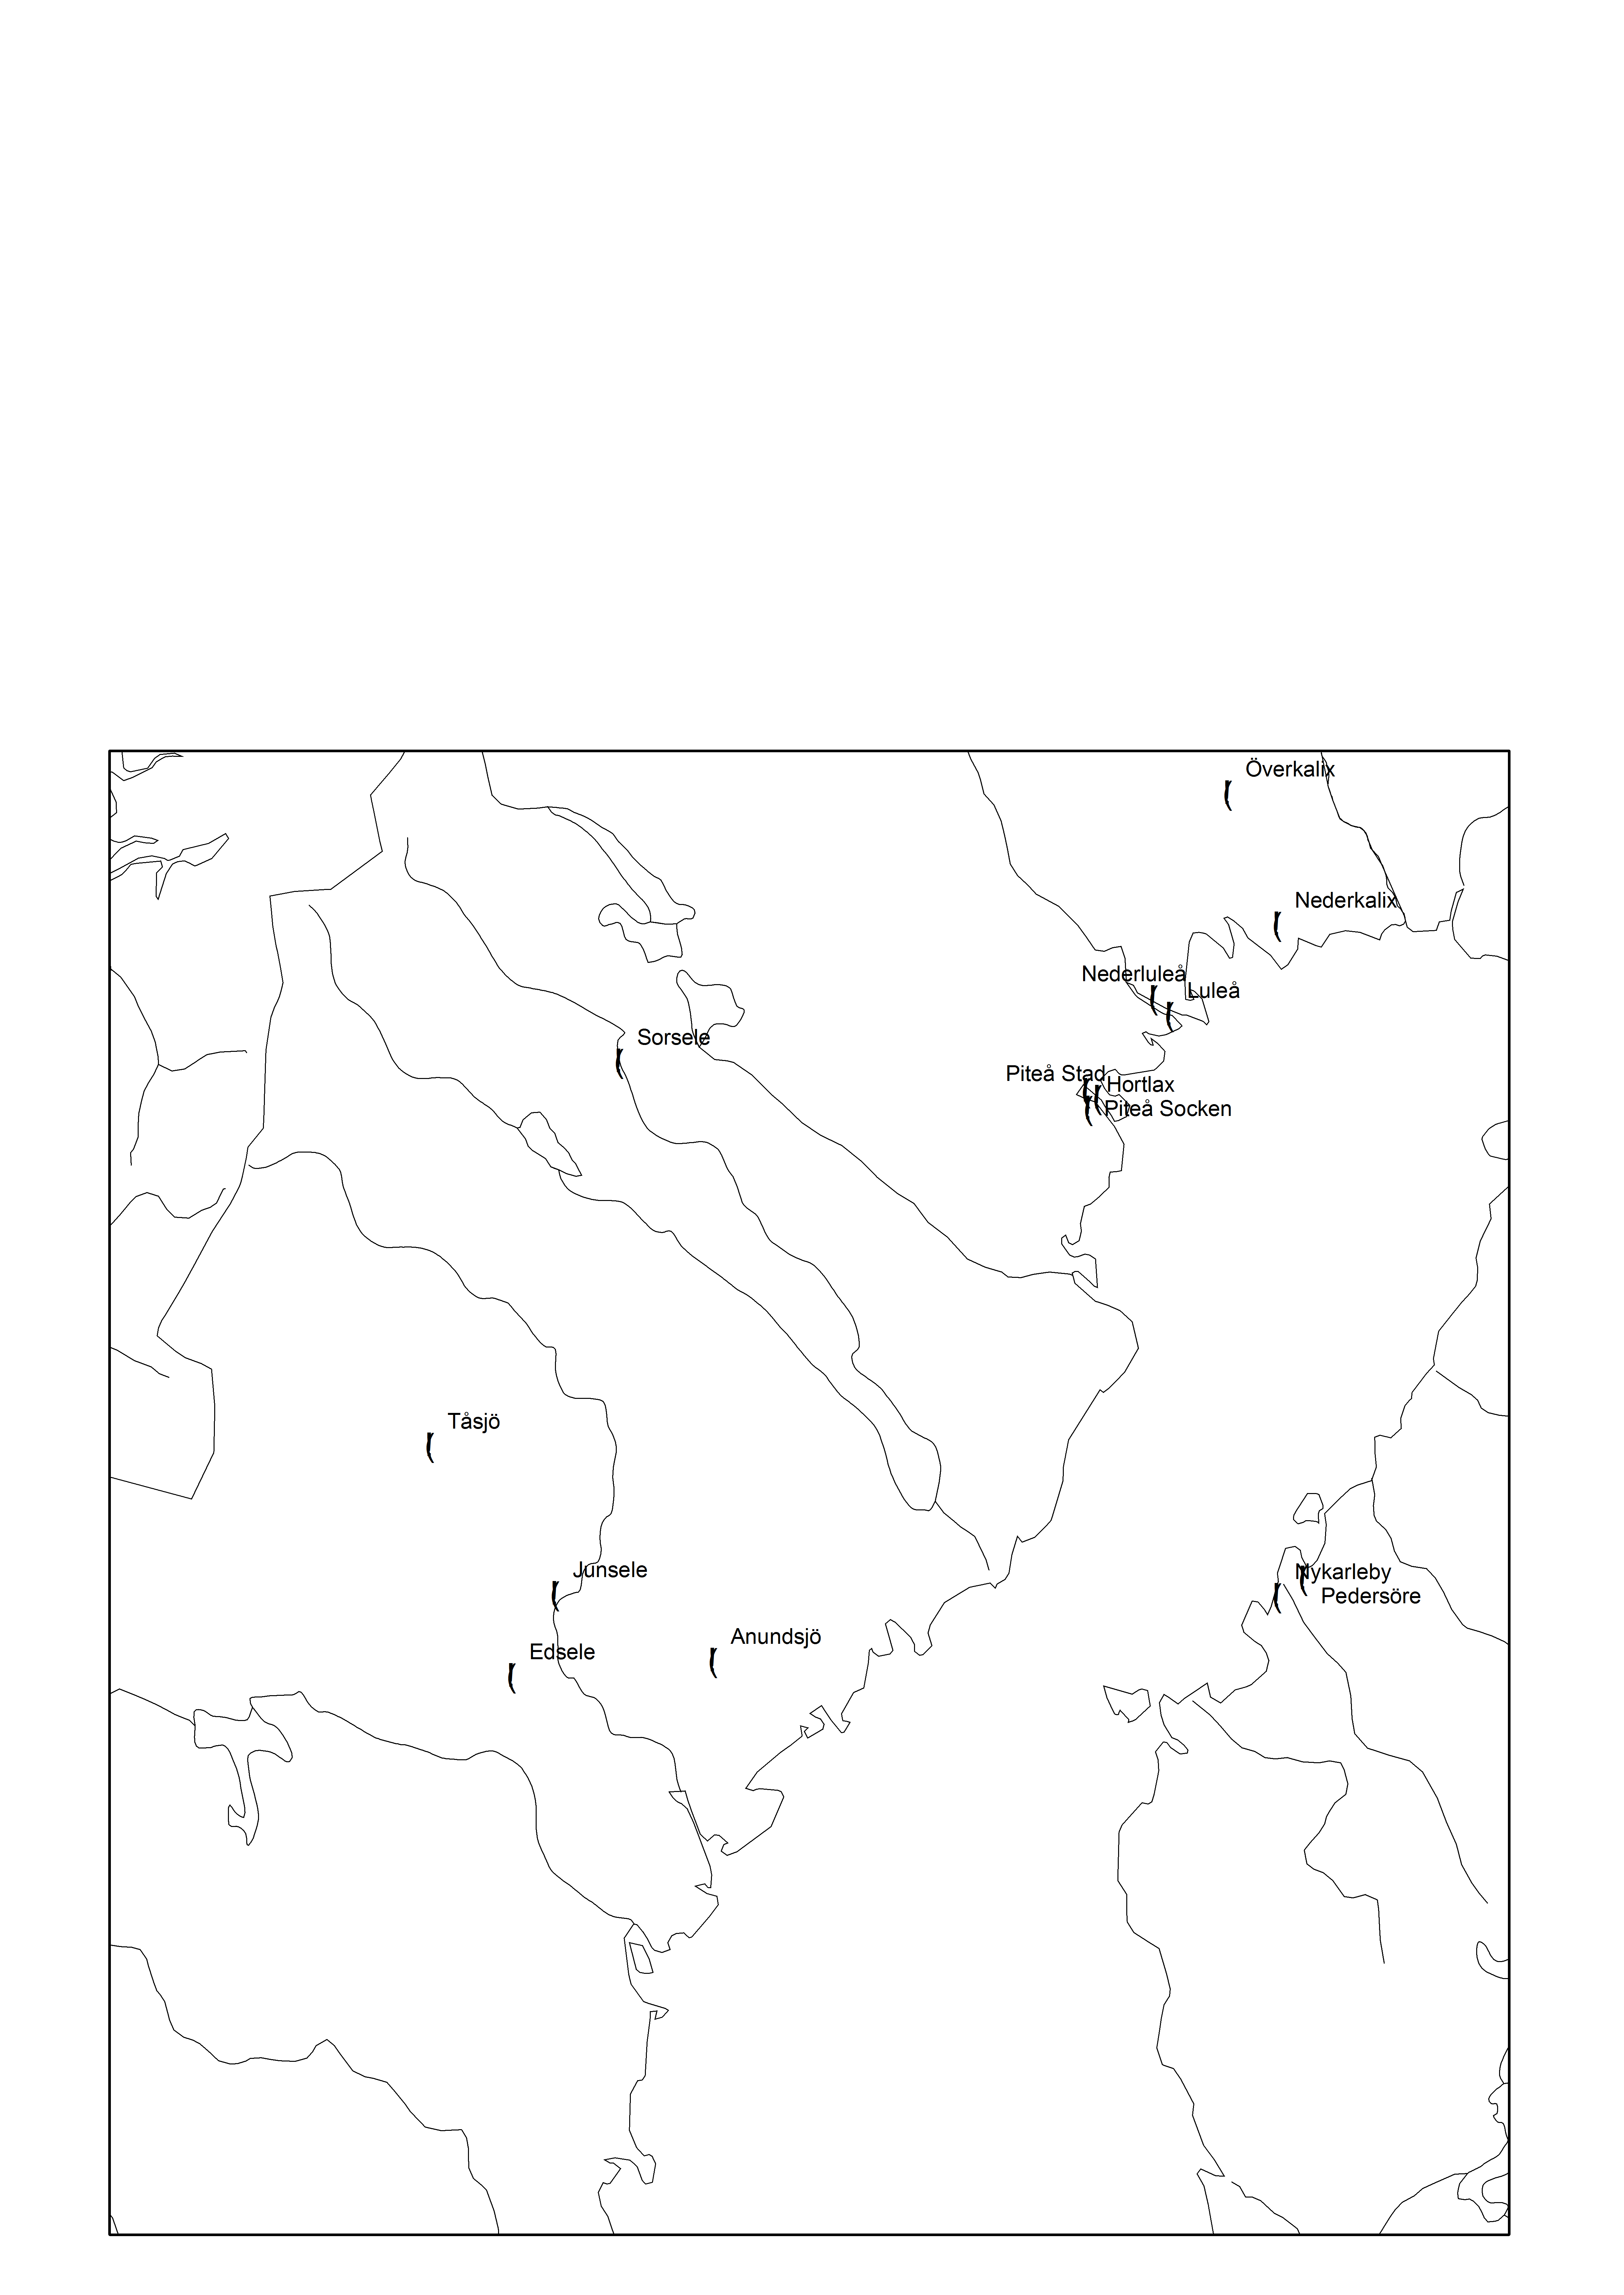
\includegraphics[height=.5\textheight]{figures/15_AttestationsofDefinites}
\caption{Attestations of definites after ‘much’.}
\label{map:12}

\end{figure}

\begin{figure}[h]
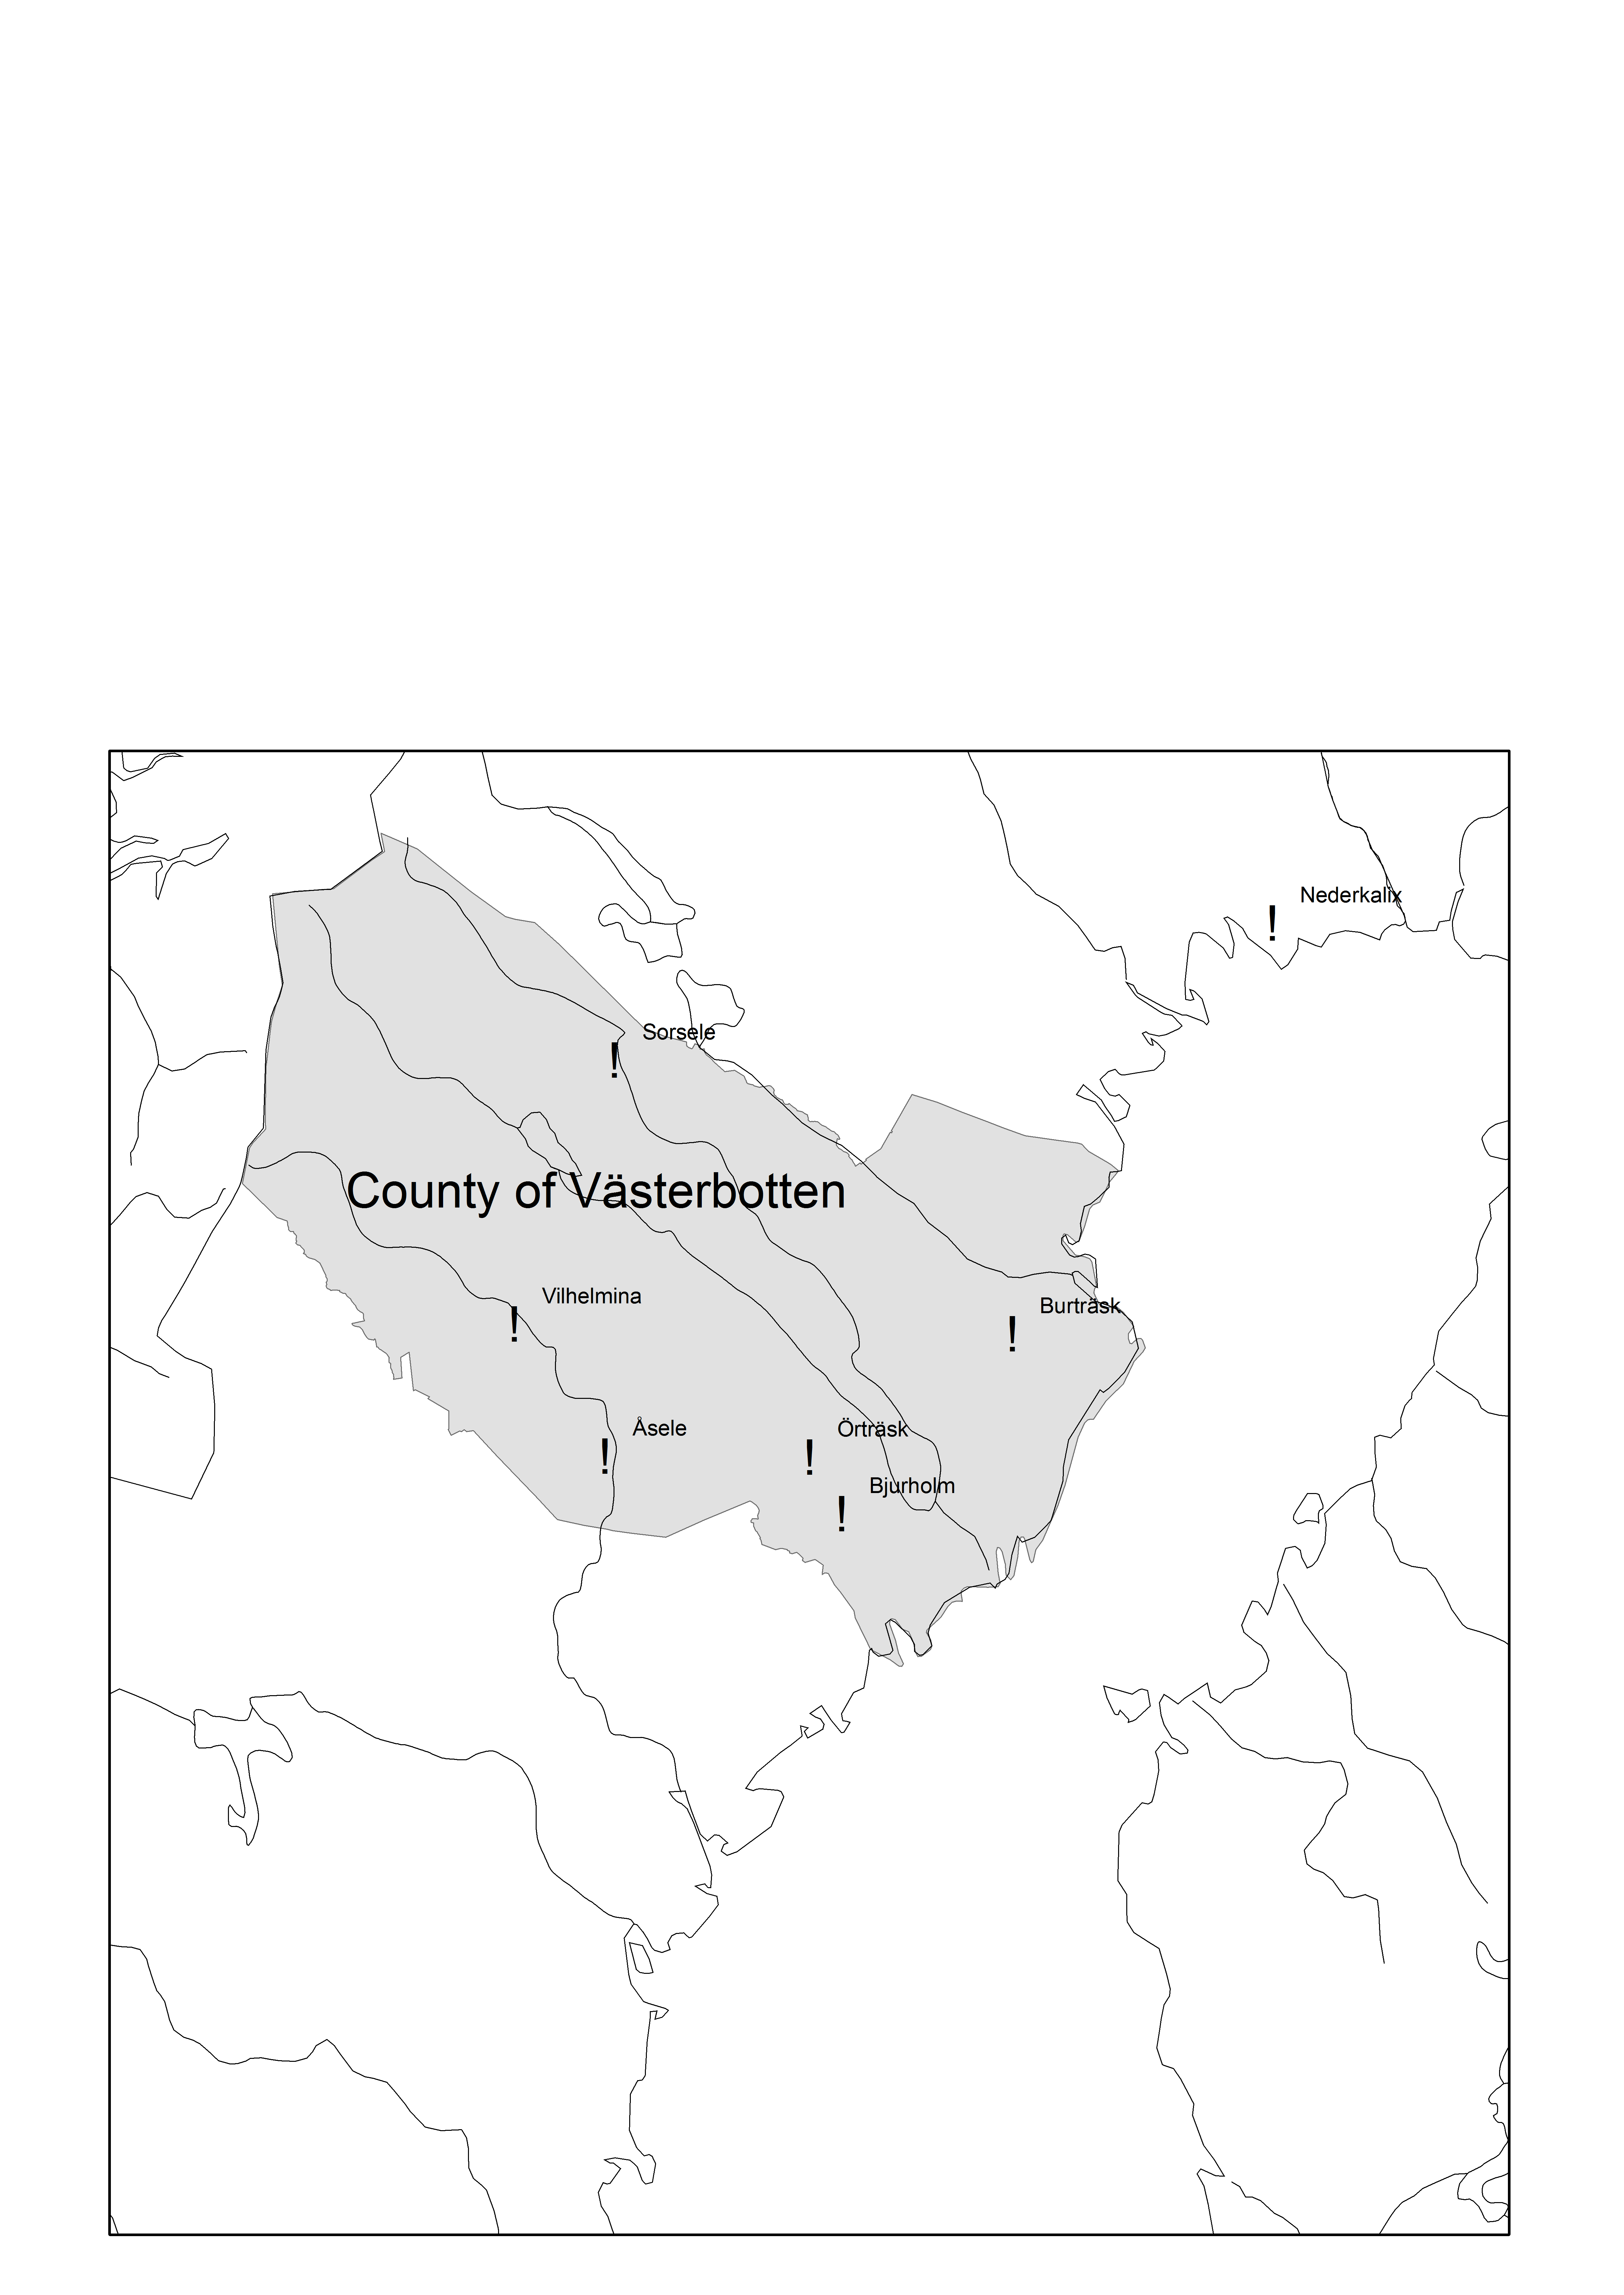
\includegraphics[height=.5\textheight]{figures/16_AttestationsofDefinitesNumerals}
\caption{Attestations of definites after numerals.}
\label{map:13}

\end{figure}

\begin{figure}[h]
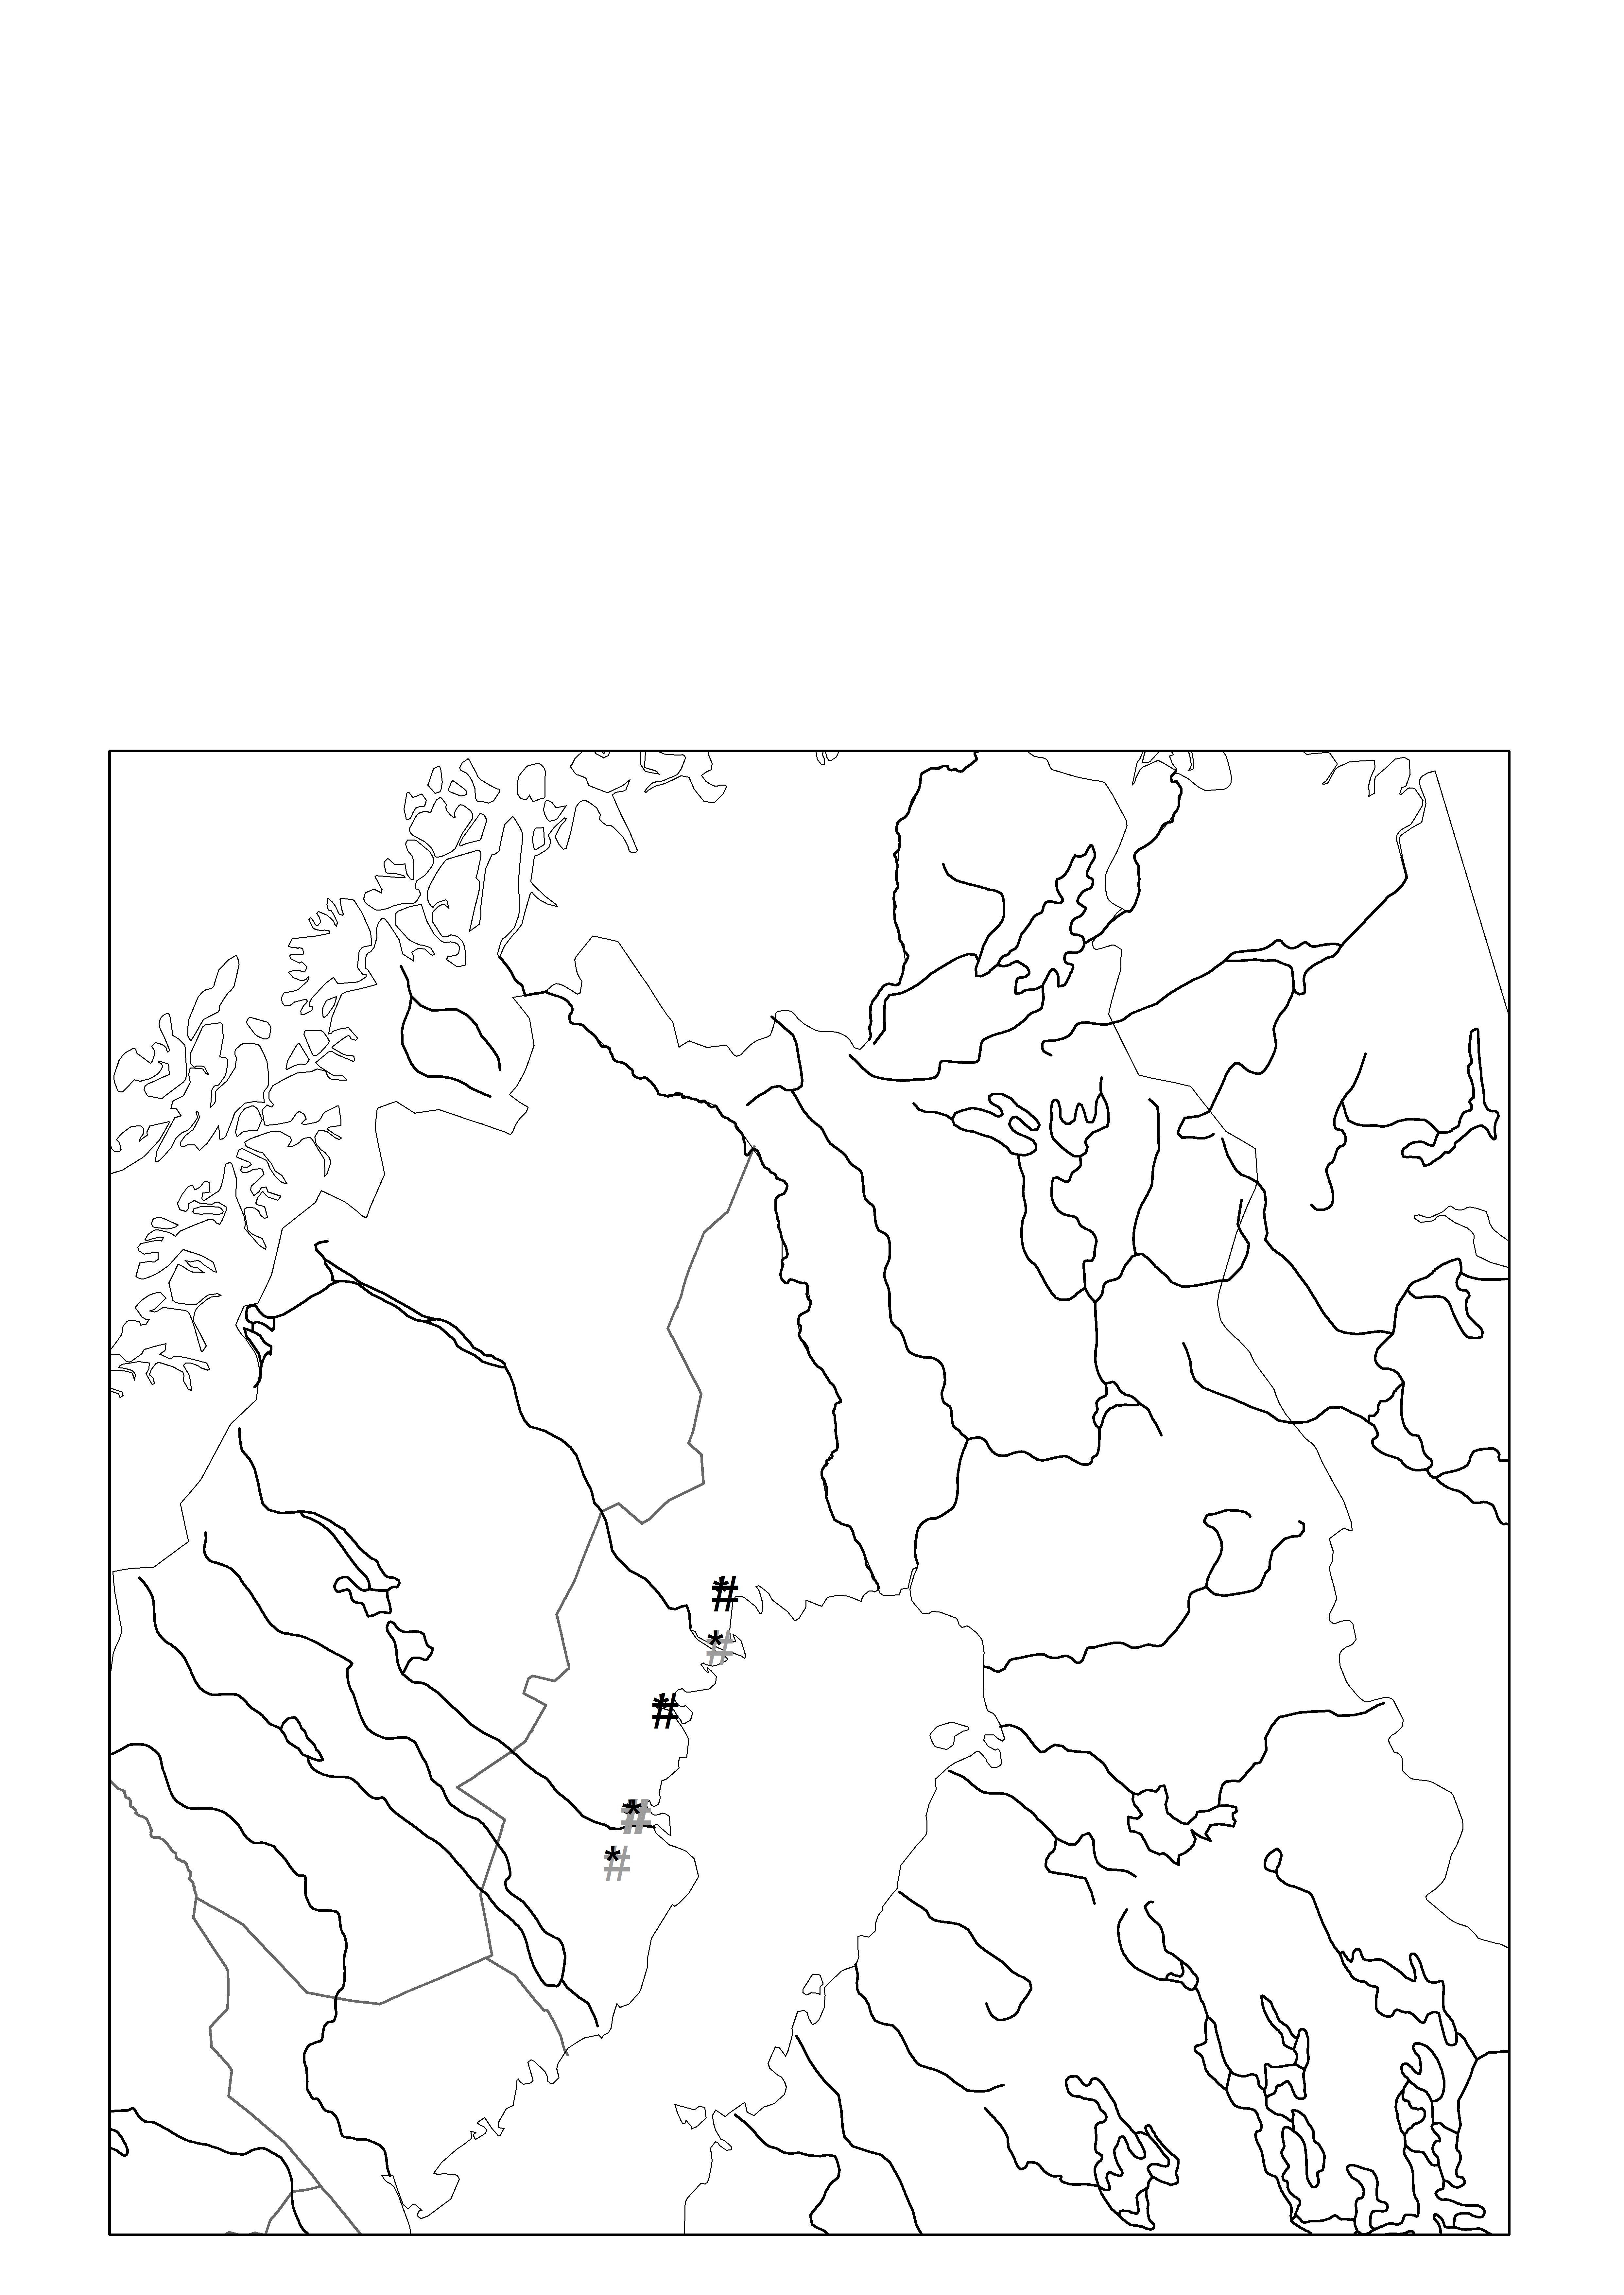
\includegraphics[height=.5\textheight]{figures/18_AttestationsofDatives}
\caption{Attestations of dative after quantifiers (black symbols: extended uses).}
\label{map:14}

\end{figure}

\begin{figure}[h]
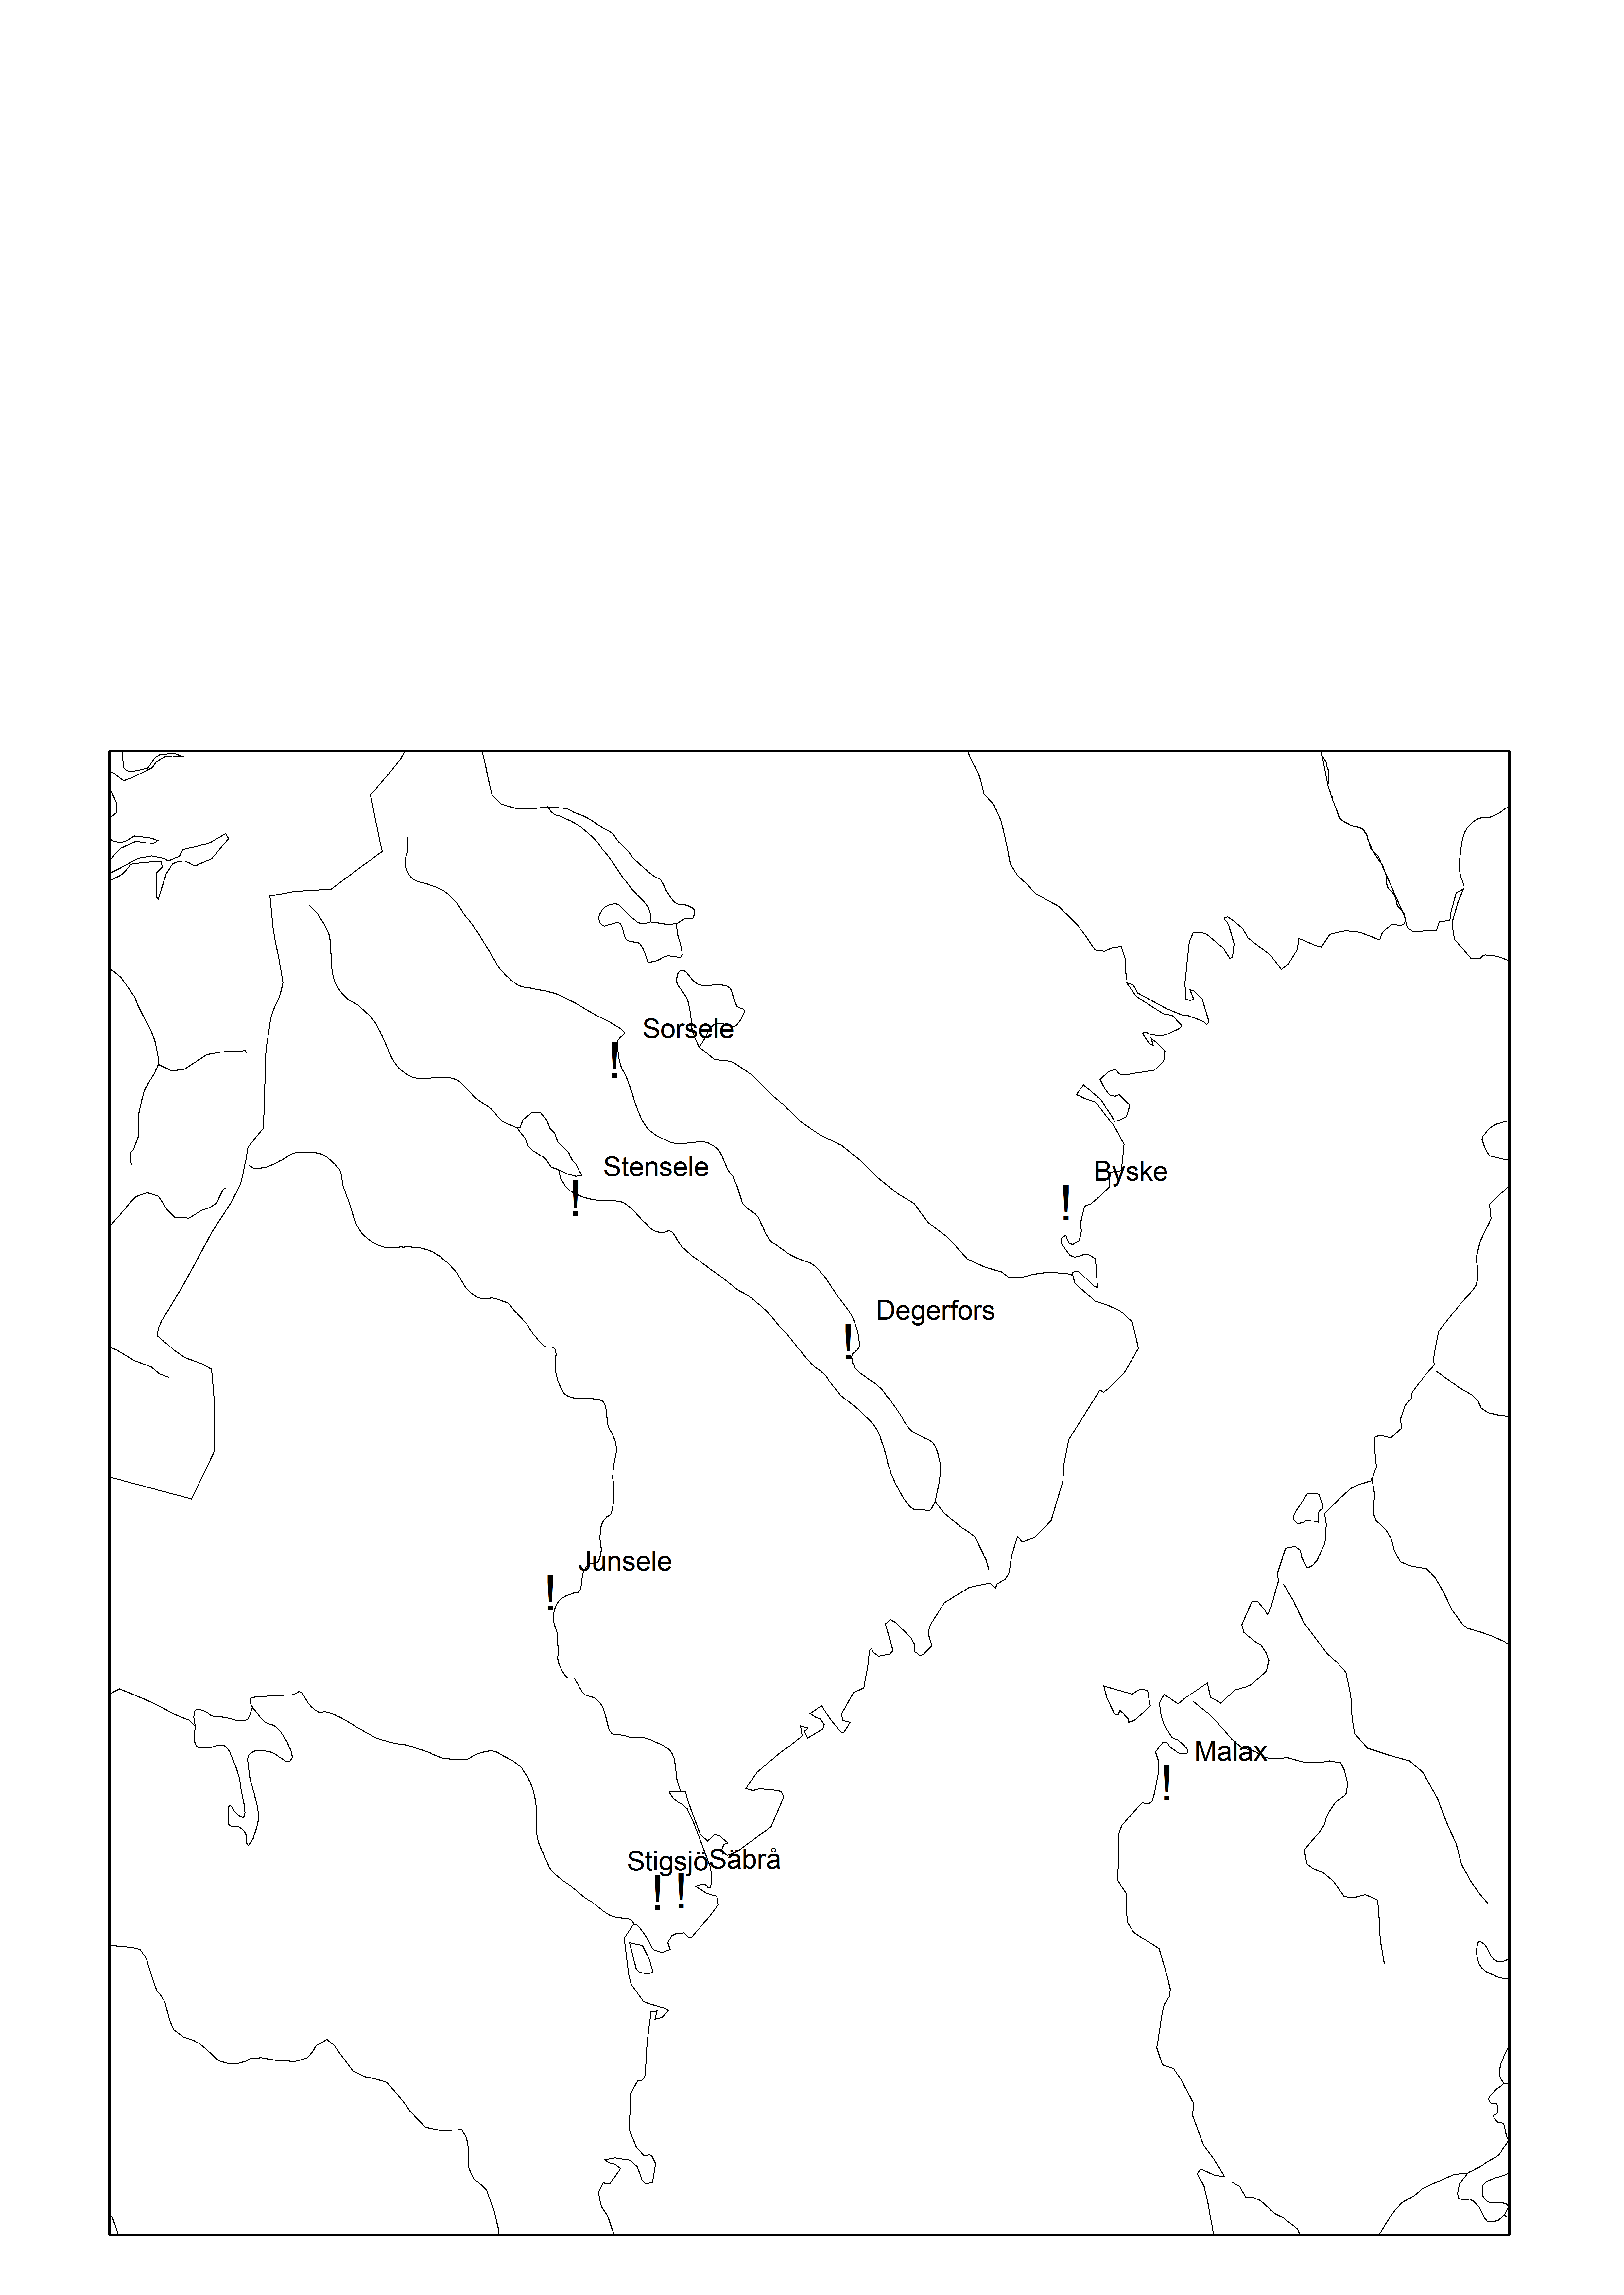
\includegraphics[height=.5\textheight]{figures/17_AttestationsAfterNa}
\caption{Attestations of definites after \textit{na}.}
\label{map:15}

\end{figure}

\subsection{ Singular count uses}
\label{sec:3.2.5}

In the peripheral area, there are also some unexpected uses of suffixed articles with singular count nouns, such as the following:

\ea %\label{} 
\langinfo{\label{bkm:Ref224102863}Älvdalen (Os)}{}{}\\
\gll Am  \textbf{est-n}.\\
have.1{\pl}  \textbf{horse-{\deff}}\\
\glt ‘We have a horse, i.e. we are horse-owners.’ (questionnaire)

\z

Such examples, which would normally take an indefinite article in English, by and large correspond to “bare nouns” in the Central Scandinavian languages e.g.

\ea %\label{} 
\langinfo{\label{bkm:Ref224102890}Swedish}{}{}\\
\gll Vi  har  \textbf{häst}.\\
we  have.{\prs}  \textbf{horse}\\
\glt ‘We have a horse, i.e. we are horse-owners.’

\z

I shall call such cases “low referentiality uses” (\citealt[3:56]{TelemanEtAl1999} “svagt referentiell betydelse”), since they share the trait that the identity of the referent is not highlighted; what is important in \REF{104}{}-\REF{105} is rather the property of owning a horse. Correspondingly, the bare noun construction in Swedish is normally used when speaking of something that it is normal to have exactly one exemplar of, including cars\footnote{ A Google search suggests that the bare noun phrase \textit{har bil} ‘has car’ is about ten times as common as \textit{har en bil} ‘has a car’ in Swedish, and of the latter the overwhelming majority were followed by a relative clause. } and telephones (at least until recently!), but excluding spaceships (because you are not expected to have one) or books (because you are expected to have several). However, the corresponding sentences with indefinite articles are also grammatical, and in fact preferred in certain contexts, e.g. if the referent is going to be important in the ensuing discourse. The articleless variant is however felt to be ungrammatical in Elfdalian (I have not been able to systematically check on other vernaculars), but conversely, the definite article is not possible in Central Scandinavian. 

From the diachronic point of view, the article-less cases of Central Scandinavian could be seen as due to an incomplete grammaticalization of the indefinite article, whereas the use of the definite article in Peripheral Swedish vernaculars is a case of grammaticalization that goes further than we would perhaps expect. Typologically, it is not wholly unique, however. While \REF{104} could not be translated into French using a definite article, there are similar examples such as \REF{106}, where a definite article is normal:

\ea %\label{} 
\langinfo{\label{bkm:Ref224102943}French}{}{}\\
\gll Nous  avons  \textbf{le} \textbf{téléphone}.\\
we  have.{\prs}.1{\pl}  \textbf{{\deff}} \textbf{telephone}\\
\glt ‘We have a (lit. the) telephone.’

\z

Cases like this are mentioned in standard grammars of French, but they tend to be subsumed under generic uses of the article (I’ll return to this question in \sectref{sec:3.4}). 

With respect to the peripheral Swedish dialect area, the low referentiality uses of definite forms are not well documented in the literature, and when examples are provided they are usually not seen as a type of their own, distinct from non-delimited uses. For instance, \citet[282]{ÅgrenEtAl1954}, after discussing uses of definite forms for “indefinite quantities” and saying that Norrlandic dialects “are very consistent in this use of the definite forms”, cite the following as “maybe particularly striking to a Standard Swedish ear”:\footnote{ “De norrländska bygdemålen är mycket konsekventa i detta bruk av bestämd form. Särskilt påfallande för ett rikssvenskt öra är måhända…”} 

\ea %\label{} 
\langinfo{Vilhelmina (SVb)}{}{}\\
\gll Sä  vi  mâka  ôss  \textbf{kâmmarn}.\\
so  we  clear.{\pst}  us  \textbf{chamber.{\deff}}\\
\glt ‘so we cleared us a chamber.’ [i.e. we made a shelter by clearing some snow]’

\z

This example, like the following ones, shows that the phenomenon may include cases that do not correspond to bare-noun constructions in Swedish: 

\ea%\label{}
\langinfo{Älvdalen (Os)}{}{}\\
\gll E  wa  \textbf{swaindjin} å  weem.\\
it  be.{\pst}  \textbf{bend.{\deff}} on  road.{\deff}.{\dat}\\
\glt ‘There was a bend in the road.’ [S12]

\z

\ea
\gll Ig  ar  gart  \textbf{stark-äln} ig.\\
I   have.{\prs}  make.{\supp}  \textbf{strong\_heel.{\deff}.{\acc}} I\\
\glt ‘I have made a strong heel’ (\citealt[95]{Levander1909})

\z

Due to restricted documentation and a rather low text-frequency, it is not so easy to establish the precise geographical distribution for the extended use of definite forms of singular count nouns, but I have found a number of examples from various ends of the Peripheral Swedish area, to be listed in the following: 

\subsubsection{Norrbothnian}
 Starting from the north, the following two translations of the same sentence from the Cat Corpus can be cited from the Kalix area:

\ea%\label{}
\langinfo{Överkalix (Kx)}{}{}\\
\gll Ji  skå  taLa  om  föR  di  mamm\\
I  shall.{\prs}  speak.{\inf}  about  for  you.{\obl}  mother\\
\gll aT  ji  ållti  hä  önske  mi  i  kätt,\\
that  I  always  have.{\prs}  want.{\supp}  me.{\obl}  {\indf}  cat\\
\gll men  he  gär  jåo  äint  änn  aT  ha  \textbf{kätta}\\
but  it  go.{\prs}  {\prag}  {\neg}  well  {{\inf}m}  have.{\inf}  \textbf{cat.{\deff}}\\
\gll da´n  båo  ini  in  höires-häos.\\
when\_one  live.{\prs}  in  one.{\dat}.{\n}  apartment house\\
\glt ‘I want to tell you, Mother, that I have always wanted to have a cat – but it isn’t possible to have a cat (lit. the cat) when you live in an apartment house.’ (Cat Corpus)

\z

\ea%\label{}
\langinfo{Nederkalix (Kx)}{}{}\\
\gll Jä  skå  tåla  åom  för  dä,  måmme\\
I  shall.{\prs}  speak.{\inf}  about  for  you.{\obl}  mother\\
\gll åt  jä  ållti  veillt  hå  i  kjaatt\\
that  I  always  want.{\supp}  have.{\inf}  {\indf}  cat  \\
\gll män  hä  gja  jo  ät  håå  \textbf{kjatta}\\
but  it  go.{\prs}  {\prag}  {\neg}  have.{\inf}  \textbf{cat.{\deff}}\\
\gll når  man  båo   ini  i  höreshöus.\\
when  one  live.{\prs}  in  {\indf}  apartment house\\
\glt (same translation as above)

\z

In \citet{Stenberg1971}, we find the following examples:

\ea%\label{}
\langinfo{Siknäs, Nederkalix (Kx)}{}{}\\
\gll\bfseries
He  fanns  jo  separatoN.\\
\bfseries
it  exist.{\pst}  {\prag}  separator.{\deff}\\
\glt ‘There was a milk separator.’ 

\z

\ea\gll\bfseries
Jåå,  hästn  har  ve  jo.\\
\bfseries
yes  horse.{\deff}  have.{\prs}  we  {\prag}\\
\glt ‘Yes, we do have a horse.’ 

\z

A transcribed text on the \textsc{DAUM} website contains a couple of clear examples from the \textit{Lulemål} area (female speaker born in 1895):

\ea %\label{} 
\langinfo{Edefors (Ll)}{}{}\\
\gll Vi  hadd  ju  åt  \textbf{j}\textit{än} \textbf{spisn} så\\
we  have.{\pst}  {\prag}  {\neg}  \textbf{iron\_stove.{\deff}} so\\
\gll en  kodd  ju  åt  b\textit{a}ka  bulla….\\
one  can.{\pst}  {\prag}  {\neg}  bake.{\inf}  bun.{\deff}.{\pl}\\
\gll Da  ve  fikk  \textbf{j}\textit{ä} \textbf{nspisn}\\
when  we  get.{\pst}  \textbf{iron\_stove.{\deff}}\\
\gll da  baka  ja  ju  wettbulla  å  pepark\textit{a}kun\\
then  bake.{\pst}  I  {\prag}  wheat\_bun.{\deff}.{\pl}  and  ginger-bread.{\deff}.{\pl}\\
\gll men  strakks  hadd  ve  barra  \textbf{öppenspisn}.\\
but  right\_away  have.{\pst}  we  only  \textbf{open\_stove.{\deff}}\\
\glt ‘As you know, we didn’t have an iron stove so we couldn’t bake buns… When we got an iron stove I used to bake wheat buns and gingerbreads, but in the beginning we had only an open fireplace.’ [S33]

\z

\subsubsection{Westrobothnian}
 In Västerbotten, there seems to be more variation in the use of singular count uses of definites than is found for non-delimited uses. Thus, \citet{BergholmEtAl1999} report that mainly older speakers used definite forms in \REF{112}. \citet{WälchliEtAl1998}, on the other hand, did not find any examples of definites at all in this sentence when using the same questionnaire.

\ea %\label{} 
\langinfo{\label{bkm:Ref224103495}Burträsk (NVb)}{}{}\\
\gll Vi  hadd  \textbf{hästn} menn  ja  vor  litn.\\
we  have.{\pst}  \textbf{horse.{\deff}} when  I   be.{\pst}  small\\
\glt ‘We had a horse when I was a kid.’ (questionnaire)

\z

In transcribed texts from Västerbotten, a few examples are found, e.g.:

\ea %\label{} 
\langinfo{Norsjö (NVb)}{}{}\\
\gll …å  för-ɭɑ’ɑi̯ŋ  se´nn  där-ɖäm  inte  hɑ’ɑdd  \textbf{tjö’ttkwɑ’ɳɑ}\\
and  for long  ago  where they  {\neg}  have.{\pst}  \textbf{meat-grinder.{\deff}}\\
\gll se  ɑ’nnvä’nnde  däm \textbf{kƚe’sta’i̯t’n}.\\
so  use.{\pst}  they  \textbf{“clothes-poker”.{\deff}}\\
\glt ‘…and long ago where they didn’t have a meat-grinder they used a \textit{klädstöt}.\footnote{ Tool used when washing clothes.} (\citealt[303]{Westerberg2004})

\z

\ea %\label{} 
\langinfo{\textit{Skelletmål} (NVb)}{}{}\\
\gll Hänna  dug  äint  för  ajn  som  ha  \textbf{julpän.} \\
this  do.{\prs}  {\neg}  for  one  that  have.{\prs}  \textbf{fly.{\deff}} \\
\glt ‘This won’t do for someone with a fly.’ (\citealt[94]{Westerlund1978})

\z

\subsubsection{Middle Norrland}
 There seem to be no clear examples from the provinces of Jämtland, Ångermanland, and Medelpad. Although it is hard to argue from the absence of evidence, something could certainly be expected to show up in the extensive text materials, so it would appear that singular count uses are not found here. This impression is strengthened by the fact that definite forms are also not found with instrumental prepositional phrases (see below). 

\subsubsection{Ostrobothnian}
 \citet[207]{Nikula1997} quotes the following examples from Närpes, exemplifying the bare noun pattern:

\ea%\label{}
\langinfo{Närpes (SOb) }{}{}\\
\gll Vi  ha:  \textbf{häst} därhäim.\\
we  have.{\prs}.{\pl}  \textbf{horse} at\_home\\
\glt ‘We have a horse at home.’

\z

\ea
\gll Ja  ha:r  no:  \textbf{moånanslyö:n}.\\
I  have.{\prs}  certainly  \textbf{monthly\_salary}\\
\glt ‘Sure, I have a monthly salary.’

\z

She seems to imply that this is the only possibility in this vernacular and explains this by the “non-referential function” of the noun phrases in question, which do not introduce a referent but rather contribute to the characterization of the subject as horse-owners and salaried employees respectively. 

\citet{ErikssonEtAl1999}, in their questionnaire investigation of Ostrobothnian, also found that the bare noun pattern was predominating. However, one informant from Munsala in northern Österbotten did produce a definite variant, together with one with an indefinite article:

\ea 
\langinfo{Munsala (NOb)}{}{}\\
	\ea { 
	\gll 	Vi  had  \textbf{hästin,} tå  ja  va  lill.\\
			we  have.{\pst}  \textbf{horse.{\deff}} when  I   be.{\pst}  small\\
	}
	\ex {
	\gll 	Vi  had  \textbf{in} \textbf{häst,} tå  ja  va  lill.\\
			we  have.{\pst}  \textbf{{\indf}} \textbf{horse} when  I  be.{\pst}  small\\
	\glt 	‘We had a horse when I was a kid.’ (questionnaire)
	}
	\z 
\z

\citet{ErikssonEtAl1999} a\textstyleBodyTextFirstChar{l}so quote a number of examples of definite-marked countable singulars from published texts:

\ea %\label{} 
\langinfo{Sideby (SOb)}{}{}\\
\gll Så  kviila  vi  \textbf{middain.} \\
so  rest.{\pst}  we  \textbf{noon.{\deff}} \\
\glt ‘Then we took a nap.’ (Standard Swedish \textit{vila middag}) [S19]

\z

\ea %\label{} 
\langinfo{Sideby (SOb)}{}{}\\
\gll Å  dåm  hav  \textbf{öitjon}.\\
and  they  have.{\prs}  \textbf{dinghy.{\deff}}\\
\glt ‘And they have a dinghy.’ [S19]

\z

\citet{Ivars2005} presents at least one fairly clear example from Närpes:

\ea %\label{} 
\langinfo{Närpes (SOb)}{}{}\\
\gll Han  ha:  ju  \textbf{brännvinsbo:den} han.  \\
he  have.{\pst}  {\prag}  \textbf{liquor-shop.{\deff}} he  \\
\glt ‘He had a liquor shop, he.’ 

\z

Thus, the use of definite forms with singular countables is fairly well documented also in Ostrobothnian, although the article-less pattern is more common in present-day usage.

\textbf{Ovansiljan}. Examples from Elfdalian have already been quoted above. Questionnaires from Orsa and Sollerön give a result which is similar to the one reported above for non-delimited uses. Thus, the majority of the informants from Orsa used the definite form in \REF{120}, whereas none from Sollerön did:

\ea %\label{} 
\langinfo{\label{bkm:Ref224103820}Orsa (Os)}{}{}\\
\gll Wi  addum  \textbf{äst’n} dö  i  wa  lit’n.\\
we  have.{\pst}.1{\pl}  \textbf{horse.{\deff}} when  I   be.{\pst}  small\\
\glt ‘We had a horse when I was a kid.’ (questionnaire)

\z

\subsubsection{Summing up}
 Like the use of definite forms after quantifiers, the extended use of definite forms with count nouns display is less well entrenched in the Peripheral Swedish area than the non-delimited type. Their absence from the Middle Norrland area is conspicuous. (Compare also the more questionable example \REF{188} from Hållnäs in Uppland below.)

\subsection{ Instrumental prepositional phrases }

\citet{Himmelmann1998} claims that articles “are generally used less frequently, and with regard to semantic and pragmatic generalisations, less consistently in adpositional phrases than in other syntactic environments (such as subject or object position)”. Manner and instrumental adverbial phrases would be a case in point, and indeed, in English, certain types of manner-characterizing prepositional phrases tend to involve bare nouns, particularly those that indicate manner of locomotion, such as \textstyleLinguisticExample{by train}, \textstyleLinguisticExample{by foot}, \textstyleLinguisticExample{by car}. In Central Scandinavian, the use of such bare nouns is considerably wider. Thus, in Swedish, the phrase \textstyleLinguisticExample{med kniv} ‘[lit.] with knife’ is much more common\footnote{ A Google count: \textit{med}\textit{ }\textit{kniv}: 14300, \textit{med en kniv}: 2820. In English, there is a parallel in the phrase \textit{by} \textit{knife}, appearing in phrases such as \textit{homicide by knife}.} than \textstyleLinguisticExample{med en kniv }‘with a knife’, and in the following sentence, the use of an indefinite article sounds definitely strange:

\ea %\label{} 
\langinfo{\label{bkm:Ref224115033}Swedish}{}{}\\
\gll Hon  äter  soppa  med  \textbf{(?en)} \textbf{  sked}.\\
she  eat.{\prs}  soup  with  \textbf{{\indf}} \textbf{spoon}\\
\glt ‘She eats soup with a spoon.’

\z

In the light of these observations and Himmelmann’s claim, it is rather unexpected to find languages where in fact \REF{121} would be translated using a definite article in the phrase ‘with a spoon’, even when it is evident that no specific spoon is being referred to. Nevertheless, in French, if the preposition \textstyleLinguisticExample{à} is chosen, it is regularly followed by the definite rather than by the indefinite article:

\ea %\label{} 
\langinfo{French}{}{}\\
\gll Elle  mange  la  soupe  à  \textbf{la} \textbf{cuillière}.\\
she  eat.{\prs}  {\deff}  soup  with  \textbf{{\deff}} \textbf{spoon}\\
\glt ‘She eats soup with a spoon.’

\z

where a definite NP is used after the preposition \textstyleLinguisticExample{à}. With this preposition, the definite article seems more or less obligatory. (Compare captions of paintings such as \textstyleLinguisticExample{Jeune fille au chèvre} ‘Young girl with a goat’). With the synonymous preposition \textstyleLinguisticExample{avec} the definite article is possible but the preferred variant appears to be with an indefinite NP:

\ea %\label{} 
\langinfo{French}{}{}\\
\gll Elle  mange  la  soupe  avec  \textbf{une} \textbf{cuillière}.\\
she  eat.{\prs}  {\deff}  soup  with  \textbf{{\indf}} \textbf{spoon}\\
\glt ‘She eats soup with a spoon.’

\z

Similarly, in the Peripheral Swedish vernaculars, instrumental phrases of this type often show up with a definite head noun. Thus, \citet[126]{Levander1909} quotes the following Elfdalian example, which he translates into Swedish using a bare noun construction (\textstyleLinguisticExample{med kniv} ‘with a knife’)

\ea %\label{} 
\langinfo{Älvdalen (Os)}{}{}\\
\gll Sjo  ur  dier  ovo  skrievað  \textbf{min} \textbf{  knaivem!}\\
see  how  they  have.{\prs}.3{\pl}  write.{\supp}  \textbf{with} \textbf{knife.{\deff}.{\dat}}\\
\glt ‘Look what they have written with a knife!’ (\citealt[125]{Levander1909})

\z

%\begin{styleTextkrper}
A modern Elfdalian example elicited by questionnaire is \REF{125}.

%\end{styleTextkrper}

\ea %\label{} 
\langinfo{\label{bkm:Ref224103303}Älvdalen (Os)}{}{}\\
\gll An  jät  supp\k{u}  \textbf{min} \textbf{  stjiedn}.\\
he  eat.{\prs}  soup.{\deff}.{\acc}  \textbf{with} \textbf{spoon.{\deff}.{\dat}}\\
\glt ‘He eats soup with a spoon.’ (questionnaire)

\z

%\begin{styleTextkrper}
However, the informant indicated that the indefinite form was also possible:

%\end{styleTextkrper}

\ea %\label{} 
\langinfo{Älvdalen (Os)}{}{}\\
\gll An  jät  supp\k{u}  \textbf{min} \textbf{  stjied}.\\
he  eat.{\prs}  soup.{\deff}.{\acc}  \textbf{with} \textbf{spoon.{\dat}}\\
\glt ‘He eats soup with a spoon.’ (questionnaire)

\z

%\begin{styleTextkrper}
From Orsa, where there were several questionnaire responses, the majority used a definite form, either in the dative or non-case marked:

%\end{styleTextkrper}

\ea %\label{} 
\langinfo{Orsa (Os)}{}{}\\
\gll An  jat  suppo  \textbf{mi} \textbf{  stjed’n/stjedi}.\\
he  eat.{\prs}  soup.{\deff}.{\acc}  \textbf{with} \textbf{spoon.{\deff}}\\
\glt ‘He eats soup with a spoon.’ (questionnaire)

\z

%\begin{styleTextkrper}
Out of four questionnaire responses from Sollerön, a definite form was given by all three informants born before 1940:

%\end{styleTextkrper}

\ea %\label{} 
\langinfo{Sollerön (Os)}{}{}\\
\gll An  jät  såppo  \textbf{minn} \textbf{  stjedn.} \\
he  eat.{\prs}  soup.{\deff}.{\acc}  \textbf{with} \textbf{spoon.{\deff}} \\
\glt ‘He eats soup with a spoon.’ (questionnaire)

\z

For Upper Norrland, we find definite forms throughout, as evidenced in questionnaires from Bjurholm, Burträsk, Norsjö, and Glommersträsk:

\ea %\label{} 
\langinfo{Bjurholm (NVb)}{}{}\\
\gll Han  ät  soppa  \textbf{ve} \textbf{skea.} \\
he  eat.{\prs}  soup.{\deff}  \textbf{with} \textbf{spoon.{\deff}} \\
\glt ‘He eats soup with a spoon.’ (questionnaire)

\z

In an early text from Överkalix, the following example is found:

\ea %\label{} 
\langinfo{Överkalix (Kx)}{}{}\\
\gll …fistsen  fik  di  takkɷ  åys  ɷpp\\
fish.{\deff}  get.{\pst}  they  almost  scoop.{\inf}  up\\
\gll \textbf{ve} \textbf{slaiven} bårti  anɷ…\\
\textbf{with} \textbf{ladle.{\deff}} from  river.{\deff}\\
\glt ‘…as for the fish, they almost had to scoop it up with a ladle from the river…’ [S17]

\z

Similar examples are found in other transcribed texts from Överkalix. 

\subsubsection{Middle Norrland}
 No examples have been found in texts from Jämtland, Ångermanland, and Medelpad. For Jämtland, informants from Lit indicate that definite forms are not possible in examples of this type.

\subsubsection{Ostrobothnian}
\citet{Hummelstedt1934} enumerates quite a few examples of the type from Närpes. 

	
\ea%\label{}
\langinfo{Närpes (SOb)}{}{}\\
	\ea {
	\gll 	Vi  sk\=ar  a  \textbf{me} \textbf{štjeron.} \\
			we  cut.{\pst}  it  \textbf{with} \textbf{sickle.{\deff}} \\
			
	\glt ‘We cut it with a sickle.’
	}
	\ex {
	\gll 	Vi  $\lambda $\=ow  \textbf{me} \textbf{lijjan.} \\
			we  cut.{\pst}  \textbf{with} \textbf{scythe.{\deff}} \\
	\glt 	‘We cut [grass] with a scythe.’
	}
	\ex {
	\gll 	Ja  tju\={ö}p  \textbf{me} \textbf{tjärron.} \\
			I  drive.{\pst}  \textbf{with} \textbf{cart.{\deff}} \\
	\glt 	‘I drove [with] a cart.’ 
	} 
	\ex {
	\gll	He  ji\=eg  me  $\lambda$ edan.\\
			it  go.PRET  \textbf{with} \textbf{sledge.{\deff}}\\
	\glt 	‘We went [lit. it went] by sledge.’ (\citealt[135]{Hummelstedt1934})
	}
	\z 
\z

\citet{Ivars2005} gives examples such as \textstyleLinguisticExample{me} \textstyleLinguisticExample{kni:vin }‘with knife.{\deff}’, \textstyleLinguisticExample{me} \textstyleLinguisticExample{li:an} ‘with scythe.{\deff}’ from South Ostrobothnian. (\citet{Nikula1997}, who also discusses Närpesmål, does not mention instrumental phrases at all.)

In the translation of the sentence ‘He eats soup with a spoon’, \citet{ErikssonEtAl1999} obtained four definite-marked responses among a total of 11 Ostrobothnian informants:

\ea 
	\ea { %\label{}
	\langinfo{Malax (SOb)}{}{}\\
	\gll 	Ha  jeter  soppu  \textbf{me} \textbf{  skeide}.\\
			he  eat.{\prs}  soup.{\deff}?  \textbf{with} \textbf{spoon.{\deff}}\\
	}
	\ex {
	\langinfo{Närpes (SOb)}{}{}\\
	\gll 	An  jäter  soppon  \textbf{me} \textbf{  sjöiden}.\\
			he  eat.{\prs}  soup.{\deff}  \textbf{with} \textbf{spoon.{\deff}}\\
	}
	\ex {
	\langinfo{Tjöck (SOb)}{}{}\\
	\gll 	Han  jiter  sopon  \textbf{me} \textbf{skeiden}.\\
			he  eat.{\prs}  soup.{\deff}  \textbf{with} \textbf{spoon.{\deff}}\\
	\glt 	‘He eats soup with a spoon.’
	}
	\z 
\z

They also quote the phrase \textstyleLinguisticExample{sloo me liian} ‘cut with a scythe’ from [S19]. 

Examples are also found in Southern Finland and Estonia, where extended uses of definites are in general quite restricted. Thus, \citet{Lundström1939} quotes examples from Nyland:

\ea%\label{}
\langinfo{Snappertuna (Ny) }{}{}\\
\gll Man  sl\=or  gräse  \textbf{me} \textbf{l\={\i}an}.\\
one  cut.{\prs}  grass.{\deff}  \textbf{with} \textbf{scythe.{\deff}}\\
\glt ‘One cuts the grass with a scythe.’ (\citealt[15]{Lundström1939}

\z

\ea
\gll Nɷ  bl\={\i}r  e  br\=a  dehäran,\\
sure  become.{\prs}  it  good  this\\
\gll bara  man  tar  innoger  t\=ag  \textbf{me} \textbf{hyviln}.\\
just  one  take.{\prs}  a\_few  take.{\pl}  \textbf{with} \textbf{plane.{\deff}}\\
\glt ‘This will surely be good, if you take a few shavings with a plane.’ (\citealt[15]{Lundström1939}

\z

In a text from Ormsö in Estonia, we find the following example:

\ea %\label{} 
\langinfo{Ormsö (Es)}{}{}\\
\gll Nu  kond  ve  bere  hlå  r\textit{å}gen  \textbf{mä} \textbf{l} \textbf{\textit{i}} \textbf{an}\\
now  can.{\pst}  we  begin.{\inf}  cut.{\inf}  rye.{\deff}  \textbf{with} \textbf{scythe.{\deff}}\\
\gll å  triske  bLai  nu  m\textit{i}ke  leta.\\
and  threshing  become.{\pst}  now  much   easy.{\cmpr}\\
\glt ‘‘Now we could begin to cut the rye with a scythe and the threshing became much easier.’ [S24]

\z

\subsubsection{Summing up}
 The use of definite forms in instrumental prepositional phrases can be considered a special case of uses with singular count nouns. The distribution of the instrumental use also is somewhat similar to that of definite forms in constructions such as ‘We have a horse’, discussed in \sectref{sec:3.2.5}. In particular, we may note that no attestations are found from Middle Norrland. On the other hand, the instrumental use extends to some areas where the other types of definite singular count nouns are not found, viz. southern Finland and Estonia. 

A possible objection (Ulrika Kvist Darnell, personal communication) is that the intended interpretation in the examples in this section is not indefinite but instead closer to something like ‘the X that I have’. It is true that if the examples had occurred in a text corpus, it would have been difficult to know exactly how they should be understood. However, the use of definites in such contexts has been noted as striking from the point of view of the standard language by several scholars who are well acquainted with the vernaculars in question. Many examples were also given as translations of Swedish sentences with indefinite noun phrases. But the fact that such examples have a somewhat fluid interpretation may be relevant in a diachronic context – see further the discussion in \sectref{sec:3.4}. 

\subsection{  “Det var kvällen”}
\label{sec:3.2.6}

\citet[16]{Delsing2003a} subsumes two different cases under “predicative constructions”: one exemplified by examples such as \textstyleLinguisticExample{hä ä sommarn} ‘it is summer’, which he calls “impersonal”, and another exemplified by “identifying constructions” such as 

\ea %\label{} 
\langinfo{\label{bkm:Ref224115132}(no location)}{}{}\\
\gll De  här  ä  \textbf{körpen}.\\
this  here  be.{\prs}  \textbf{pick.{\deff}}\\
\glt ‘This is a pick.’

\z

It appears, though, that these two patterns have rather different geographic distributions. Examples like \REF{135}, which are rather close to citation uses (see \sectref{sec:3.2.1}), are not to my knowledge attested outside the area where extended uses of definites are normally found, but “impersonal” constructions characterized by the pattern

%\begin{styleBlockQuote}
impersonal subject ‘it’ + copular verb ‘be’ or ‘become’ + noun denoting a temporal interval

%\end{styleBlockQuote}

are quite widespread in Scandinavia. In the Swedish dialect area, examples can thus be found not only in Härjedalen, Västerdalarna, Dalabergslagen and Åboland, all close to the extended definite area, but also in south-western Sweden (the provinces of Halland and Bohuslän): 

\ea %\label{} 
\langinfo{Träslövsläge (Hl)}{}{}\\
\gll Nu  borja  här  a  bli  \textbf{kwälen,} \\
now  begin.{\pst}  here  {{\inf}m}  become.{\inf}  \textbf{evening.{\deff}} \\
\gll a  sola  gick  nair  i  sjön.\\
and  sun.{\deff}  go.{\pst}  down  in  lake.{\deff}\\
\glt ‘Now evening was coming (lit. it started to become the evening), and the sun set in the lake.’ (Cat Corpus)

\z

\ea %\label{} 
\langinfo{Sotenäs (Bo)}{}{}\\
\gll Dä  hôllte  pô  ô  b?i  \textbf{vårn} no,\\
it  hold.{\pst}  on  {{\inf}m}  become.{\inf}  \textbf{spring.{\deff}} now\\
\gll dä  kjännte  Pissen.\\
that  feel.{\pst}  pussycat.{\deff}\\
\glt ‘Spring was coming (lit. it was becoming spring), Cat felt that.’ (Cat Corpus)

\z

\ea %\label{} 
\langinfo{Östmark (Vm)}{}{}\\
\gll Nu  ä  dä  snart  \textbf{sommarn}.\\
now  be.{\prs}  it  soon  \textbf{summer.{\deff}}\\
\glt ‘Now it will soon be summer.’ (\citealt{Broberg1936}

\z

\ea %\label{} 
\langinfo{Transtrand (Vd) }{}{}\\
\gll Hä  vaL  snart  \textbf{vintern}.\\
it  become.{\prs}  soon  \textbf{winter.{\deff}}\\
\glt ‘It will soon be winter.’ (questionnaire)

\z

\ea %\label{} 
\langinfo{Houtskär (Åb)}{}{}\\
\gll N\=or  he  bǣ7ei  \textbf{kv} \textbf{\=e} \textbf{ldinj}\\
when  it  become.{\pst}  \textbf{evening.{\deff}}\\
\gll o  in  k\=om  heim  me  f\=orenj…\\
and  he  come.{\pst}  home  with  sheep.{\deff}.{\pl}\\
\glt ‘When evening came and he came home with the sheep…’ (\citealt[38]{Lundell1936})

\z

Delsing mentions a Norwegian informant from Trøndelag who accepts examples of this type, giving the impression that it is locally restricted in Norwegian. In fact, the construction is well represented in written Norwegian, both Bokmål and Nynorsk. The following example is from the Nynorsk part of the “Norsk Tekstarkiv”: 

\ea %\label{} 
\langinfo{Nynorsk Norwegian}{}{}\\
\gll Det vart  \textbf{kvelden} og  det  vart  \textbf{natta} på  nytt.\\ % \href{http://kh.hd.uib.no/cgi-dos/roman-nn.bat?P3C383000#here}{Det}
it  become.{\pst}  \textbf{evening.{\deff}} and  it  become.{\pst}  \textbf{night.{\deff}} on  new\\
\glt ‘Evening came and it became night again.’ [S29]

\z

%\begin{styleTextkrper}
An Internet example in Bokmål: 

%\end{styleTextkrper}

\ea %\label{} 
\langinfo{Bokmål Norwegian}{}{}\\
\gll Da  det  ble  \textbf{kvelden} \\
when  it  become.{\pst}  \textbf{evening.{\deff}} \\
\gll hadde  bortimot  250  shaman’er\\
have.{\pst}  around  250  shaman.{\pl}\\
\gll samlet  seg  rundt  slangen  og  kvinnen…\\
collect.{\pp}  {\refl}.3{\pl}  around  snake.{\deff}  and  woman.{\deff}\\
\glt ‘When evening came, around 250 shamans had collected around the snake and the woman…’ (Internet)

\z

The pattern does not seem to be possible in Danish or in the southernmost Swedish provinces (although it goes as far south as Halland). Its wide distribution makes it somewhat unlikely that it has spread together with the other extended uses of definite forms, which are less widespread. 

\subsection{ Various minor patterns}

\subsubsection{Illnesses}
 In the literature, names of illnesses are sometimes provided as examples where definite forms are used in vernaculars more extensively than in Swedish. Thus: 

\ea %\label{} 
\langinfo{Pyttis (Ny) }{}{}\\
\gll Bɷonen  har  jɷ  \textbf{c(ikhɷston}.\\
child.{\deff}.{\pl}  have.{\prs}  {\prag}  \textbf{whooping-cough.{\deff}}\\
\glt ‘The children have got whooping-cough.’ (\citealt[11]{Lundström1939}

\z

\ea %\label{} 
\langinfo{Östmark (Vm)}{}{}\\
\gll Han  ä  ill  kommen  ta  \textbf{jekta}.\\
he  be.{\prs}  badly  come.{\pp}  of  \textbf{gout.{\deff}}\\
  ‘He is suffering badly from gout’ (\citealt{Broberg1936})
\z 
  
\ea %\label{} 
\langinfo{Sollerön (Os) }{}{}\\
\gll I  a  fänndji  \textbf{ålldi.} \\
I  have.{\prs}  get.{\supp}  \textbf{stitch.{\deff}} \\
\glt ‘I have got a stitch in my side.’ (\citealt[285]{AnderssonEtAl1999})

\z

It seems hard to generalize here, though, since names of illnesses tend to behave idiosyncratically in many languages, including English – thus, \textstyleLinguisticExample{flu} is preferably used with the article but the synonymous \textstyleLinguisticExample{influenza} without.

\textbf{Measure phrases}. Definite forms also sometimes show up in phrases denoting measurements of time, weight, etc. \citet[9]{Lundström1939} provides a number of examples from Nyland: 

\ea
	\ea {
	\langinfo{Pojo (Ny)}{}{}\\
	{}[Hur länge räcker det till Lovisa?]\\
	\gll 	\textbf{Timmen} o  femton.\\
			\textbf{hour.{\deff}} and  fifteen\\
	\glt 	‘[How far is it to Lovisa?] - One hour fifteen.’
	}
	
	\ex {
	\langinfo{Borgå (Ny)}{}{}\\
	\gll	Han  c(\={ö}rd  \textbf{på} \textbf{t} \textbf{\={\i}} \textbf{man}.\\
			he  drive.{\pst}  \textbf{on} \textbf{hour.{\deff}}\\
	\glt 	‘He drove [the distance] in an hour.’
	}
	\z
\z 
	
%\begin{styleTextkrper}
In the Cat Corpus, I have only found one clear example from Överkalix (all the other vernaculars have an indefinite NP in the corresponding sentence):

%\end{styleTextkrper}

\ea %\label{} 
\langinfo{Överkalix (Kx) }{}{}\\
\gll He  dråo  nestan  \textbf{haL(e)v-täimen}\\
it  take.{\pst}  almost  \textbf{half-hour.{\deff}}\\
\gll enan  fressn  tåoRs  koma  främm.\\
before  tomcat.{\deff}  dare.{\pst}  come.{\inf}  fore\\
\glt ‘It took almost half an hour before Cat dared come out.’ (Cat Corpus)

\z

\subsection{ Preproprial articles}
\label{sec:3.2.8}

What is most appropriately called preproprial articles are used widely in Scandinavia. Preproprial articles are identical in form to third person pronouns – either full forms, which is common in Norway, or reduced (clitic) forms, as is the normal case in Sweden: \textstyleLinguisticExample{a Brita} ‘Brita’, \textstyleLinguisticExample{n Erik }‘Erik’. 

In most colloquial varieties of Swedish, third person pronouns can be used in front of proper names but then with a rather clear pragmatic effect: \textstyleLinguisticExample{han Erik} ‘that person Erik you know’. No such effect is found in the vernaculars where preproprial articles in the proper sense are used, rather they are normally obligatory with persons’ given names and with name-like uses of kin terms. They normally do not occur with surnames (which may instead have “postproprial” articles, see below). They do not appear when names are used metalinguistically (‘His name is…’) or as vocatives. 

\citet[21]{Delsing2003a} claims that in many vernaculars, preproprial articles are normally used only to refer to persons with whom the speaker is acquainted. It is not clear how this claim should be reconciled with the obligatory character of the articles, which he also mentions. In her study of the use of preproprial articles, \citet{Törnqvist2002} quotes several earlier works on Norwegian dialects in which the use is said to be unrestricted, and also a wide range of examples from Swedish vernaculars of the use of preproprial articles to refer to unacquainted referents. The reluctance that Delsing has found in some dialects against using preproprial articles with names such as \textstyleLinguisticExample{Jesus} and \textstyleLinguisticExample{Elvis} should perhaps be explained by their cultural foreignness rather than by the relationship between the speaker and their referents. 

According to \citet[21]{Delsing2003a}, preproprial articles are used generally in Norrland excluding Hälsingland and Gästrikland, in Västerdalarna and northern Värmland, and in most of Norway, excluding an area in the south and bilingual areas in the north. This is in full accordance with other statements in other sources and with the usage reflected in texts that I have seen, in particular the Cat Corpus. Delsing also says that they are used “sometimes” in Faroese and “optionally” in Icelandic spoken language. It can be seen that the distribution of preproprial articles overlaps significantly with that of extended uses of definite forms, but there are also some striking differences. Thus, if we compare the area where preproprial articles are obligatory with the area where non-delimited uses of definite forms are common, we can see that they overlap in Upper and Middle Norrland, that is, in the provinces of Jämtland and Ångermanland and the Westrobothnian and Norrbothnian dialect areas. Outside this zone, however, there is no location where the two phenomena co-exist. Thus, preproprial articles are found in most of Norway and along the Norwegian border all the way from northern Värmland and northwards except in Ovansiljan – the southern stronghold of non-delimited uses of definite forms. On the other side of the Baltic, Ostrobothnian behaves like the Ovansiljan vernaculars in these two regards. These facts suggest that preproprial articles and extended uses of definite forms have separate histories of origin.

Looking back in time, I do not know of any very old attestations of preproprial articles from Swedish vernaculars, but I have found several older texts in the Norwegian Diplomatarium with uses of pronouns that look very much like preproprial articles. One such text, consisting of one long sentence with no less than five occurrences of the pattern Pronoun+Proper Name, is rendered in the Appendix. It dates from 1430 – unfortunately, the location is not known. It thus appears that the usage was already fairly firmly established in at least some Norwegian varieties in medieval times. This, together with the geographical distribution in the Swedish dialectal area, suggests a spread from Norway, perhaps most probably from Trøndelag.

Proper names also sometimes show up with definite suffixes (called “postproprial articles” by \citealt[23]{Delsing2003a}) This usage appears to be less systematic and is most common with surnames (occasionally even in more standard varieties of Swedish). With kin terms, definite suffixes are found in Upper Norrlandic vernaculars where Standard Swedish has a bare form and many other vernaculars have preproprial articles. Compare the following examples:

\ea%\label{}
\langinfo{Sävar (SVb)}{}{}\\
\gll \textbf{Mormora} vart  alldess  rö  oppi  öga.\\
\textbf{Granny.{\deff}} become.{\pst}  quite  red  in  eye.{\deff}.{\pl}\\
\glt ‘Granny’s eyes became quite red.’ (Cat Corpus)

\z

\ea%\label{}
\langinfo{Malung (Vd)}{}{}\\
\gll \textbf{O} \textbf{Mormor} vaǦD  âlldeles  rö  i  ögon.\\
\textbf{{\pda}.{\f}} \textbf{Granny} become.{\pst}  quite  red  in  eye.{\deff}.{\pl}\\
\glt ‘Granny’s eyes became quite red.’ (Cat Corpus)

\z

\ea%\label{}
\langinfo{Swedish}{}{}\\
\gll \textbf{Mormor} blev  alldeles  röd  i  ögonen.\\
\textbf{Granny} become.{\pst}  quite  red  in  eye.{\deff}.{\pl}\\
\glt ‘Granny’s face became quite red.’ 

\z

The fourth logical possibility – both a preproprial article and a definite suffix on the same noun – is so far unattested in any variety (\citealt{Törnqvist2002}). 

\subsection{ Postadjectival articles}

Some Scandinavian dialects feature indefinite NPs according to the pattern exemplified by \textstyleLinguisticExample{en stor en bil }‘a big car’, where there is, in addition to the usual preposed indefinite article, another one between the adjective and the noun. According to \citet[46]{Delsing2003a}, the construction is found in Norway from southern Trøndelag and northwards, and in Sweden in Västerbotten, Ångermanland, Medelpad, and Jämtland. There is evidence to suggest, however, that the phenomenon had a wider distribution in earlier times. Thus, Delsing himself mentions an example from 18\textsuperscript{th} century Norrbothnian, and I have found a couple of attestations also in 18\textsuperscript{th} century Dalecarlian texts, such as the following from 1730: 

\ea %\label{} 
\langinfo{Dalecarlian (18\textsuperscript{th} century)}{}{}\\
\gll Kullur  der  giärå  ‘n  \textbf{jen} \textbf{snoggan} \textbf{jen} \textbf{krantz}\\
girl.{\pl}  there  make.{\prs}.3{\pl}  him.{\dat}  \textbf{{\indf}} \textbf{neat.{\acc}} \textbf{{\pia}} \textbf{laurel}\\
\gll um  missommors  nåti\\
about  midsummer.{\gen}  night.{\dat}\\
\glt ‘Girls there make a neat laurel for him in the midsummer night’ [S26]

\z

Delsing notes that it is sometimes hard to tell postadjectival articles from inflectional suffixes on the adjective. He claims that a suffixal analysis is more adequate in most provinces further south, as well as east of the Baltic. 

\subsection{ Summary of geographical distribution of extended uses}

We have seen that there are several different types of extended uses of definite forms in the Peripheral Swedish area, which vary to some extent in their geographical distribution. Some of the types, notably the pattern \textstyleLinguisticExample{Det är sommaren} ‘It is the summer’  and (to a somewhat lesser extent) generic uses of definites, go beyond the Peripheral Swedish area, being found also in Norway and/or southern Sweden. For the geographically more restricted uses, we can identify a few core areas: a large northern one, comprised of the provinces of Norrbotten, Västerbotten, Ångermanland, Jämtland, and Österbotten, and a smaller southern one, basically restricted to the Ovansiljan region in Dalarna. Sporadic attestations elsewhere suggest that the core areas were earlier more extensive.

\section{ Some earlier attempts to explain the extended uses of definite forms}
\subsection{ Holmberg \& Sandström}

In a paper written in Swedish, \citet{HolmbergEtAl2003} try to give a unified generative treatment of many of the phenomena discussed in this book. The title of their contribution is, in translation, “What is particular with Northern Swedish noun phrases?”. By “Northern Swedish” (\textstyleLinguisticExample{nordsvenska}), they are actually referring to a not precisely specified group of dialects in Västerbotten and the parts of Ångermanland and Norrbotten that border on the former province, said to have the following properties: 1) preproprial articles, 2) postposed possessives, 3) preposed possessives with definite head nouns, 4) postposed demonstratives, 5) adjectival incorporation, 6) suffixed definite articles on adjectives in noun phrases without a lexical head, 7) definite forms of generic nouns, 8) definite forms of “partitive” plurals and mass nouns.

Holmberg \& Sandström admit that these features do not always occur together, and that some of them also occur outside the “Northern Swedish” area. “However, there are a number of Westrobothnian dialects which display all the features, and we shall show that their combination is not accidental but on the contrary, a consistent language variety” (\citealt[87]{HolmbergEtAl2003}, my translation).

Holmberg \& Sandström adhere to the analysis of noun phrases in which they are projections of a functional category D or “determiner”, which has the consequence that in a noun phrase such as \textstyleLinguisticExample{the house}, it is \textstyleLinguisticExample{the} rather than \textstyleLinguisticExample{house} that is the head. They suggest that a major difference between Northern Swedish and other Scandinavian varieties, such as Standard Swedish, lies in the status of definite articles: the postposed article in “Northern Swedish” is a clitic, “base-generated in D [determiner position]”, whereas in Standard Swedish it is an inflectional suffix, “base-generated on [the] N[oun]”. Another difference, relating to the first, is that Northern Swedish, like the Romance languages, requires that the D-position always be filled (that is, it is realized overtly).

Let us see how these properties are used to explain the eight phenomena enumerated above. 

The D-position can, essentially, be filled in two ways: either by a base-generated determiner, or by moving the head noun (as in the figure above). The first way is seen in preproprial articles, the second in postposed demonstratives and possessives, where the head noun supposedly moves across the postposed element in order to fill the D-position. Definite adjectives in “Northern Swedish” have to be incorporated because if they appeared separately from the noun they would have to agree with it – and they don’t. 

In the case of adjectives in noun phrases without a lexical head, it is assumed that the empty element \textstyleLinguisticExample{pro} [which is the head of the NP] moves to D and the adjective is incorporated into it. 

Definite suffixes on generic nouns and “partitive” plurals and mass nouns are explained by the requirement that the D-position be filled, in the relevant cases by a definite suffix that attracts the head noun of the noun phrase. 

Holmberg \& Sandström suggest that the properties of North Swedish have developed in two steps. In the first step, the definite article is reinterpreted as a Romance-style clitic in D (the determiner position) to which a noun has to move – a clitic needs a host. This gives rise to movement of all definite nouns to D. In the second step, language-acquiring children choose to interpret this movement as depending on a requirement that D must always be filled, which gives rise to “generic and partitive articles”. 

One major problem with Holmberg \& Sandström’s theory is how to apply it to dialects in which not all properties enumerated above are present. We can note that Norwegian vernaculars tend to have preproprial articles and postposed possessives but in general lack the extended uses of definite forms found in Northern Sweden. Conversely, the Ovansiljan vernaculars lack preproprial articles and postposed demonstratives, although they display most of the other properties. This means that the evidence for movement of nouns to D is considerably weaker in those vernaculars. Moreover, the differences in geographical distribution between e.g. preproprial articles and extended uses of definites suggest that they also have different historical origins). 

Notice further that nouns preceded by demonstratives generally take definite suffixes in all Swedish spoken varieties, e.g.

\ea %\label{} 
\langinfo{Älvdalen (Os)}{}{}\\
\gll an  dar  kalln\\
that  there  man.{\deff}\\
\glt ‘that man’

\z

If the definite suffix originates in the D position, it is not clear how it could end up on the noun in such noun phrases. The same can be said of noun phrases with definite nouns following quantifiers, as described in \sectref{sec:3.2.4}, which are common in the area focused on by Holmberg \& Sandström, although they do not mention them. It would appear that those noun phrases have both an unfilled D and a definite suffix in an unexpected position where it cannot be accounted for by the demand for a filled D. (One could probably say more or less the same of possessives with definite head nouns which are listed as one of the interesting properties by Holmberg \& Sandström but are not further commented upon in the paper.)

Consider also the explanation of the preproprial articles, where the condition on filled D’s is also invoked. Holmberg \& Sandström, quoting Longobardi (1994, 1995), note that in Romance languages, which are also supposed to have the filled-D condition, some varieties (e.g. Standard Italian) do and others (e.g. some Italian vernaculars) do not have preproprial articles. It thus has to be assumed that, in a language with the filled-D condition, there are two possibilities: either there is a preproprial article or the proper name moves to D. What is excluded, they say, is for a proper name that remains in situ to lack an article. The problem here is that the movement of proper names to D is in general “invisible” since the proper name is in initial position in the NP anyway. Thus, the filled-D condition could be said to be vacuously fulfilled for proper names even in languages such as Elfdalian and Swedish. This fact raises some doubt about the motivation for the introduction of preproprial articles. If the filled-D condition is fulfilled anyway, why should a language bother to introduce them? Indeed, since there is more than one solution compatible with the filled-D condition, it may be said that this parameter underdetermines the behaviour of proper noun phrases. Notice that apparently one and the same language can choose different solutions: it is generally only with first names that preproprial articles are obligatory. 

With respect to the claim that definite suffixes are clitics in Peripheral Swedish vernacular, it may be noted that clitics generally represent less advanced stages in grammaticalization processes, and the development from inflectional ending to clitic is rather uncommon. It is generally assumed that the Scandinavian definite articles have passed through a clitic stage, and later been fused with their head nouns – that is, the opposite direction. The wider range of uses of definite forms in Peripheral Swedish vernaculars compared to Central Scandinavian rather suggests that the Peripheral Swedish forms have advanced further in the grammaticalization process. There is little indication of synchronic clitic-like behaviour. One may for instance compare the definite suffixes to the marker of the \textstyleLinguisticExample{s}{}-genitive, which in Central Scandinavian may be added to the last constituent of the noun phrase even if that is not the head noun. The same holds for the possessive marker \textstyleLinguisticExample{es} in Elfdalian (see \sectref{sec:5.4.2}). No such thing is possible with definite suffixes in Peripheral Swedish vernaculars. Also, phenomena such as portmanteau expression of definiteness, number and case, neutralization of the definiteness distinction (see \sectref{sec:3.1.5}), and variation between different declension classes are not typical of clitics. The fact that indeclinable nouns such as \textstyleLinguisticExample{kaffi} ‘coffee’ take zero definite endings is also unexpected if the definite suffix is a clitic. Admittedly, it is true that the fact that headless adjectives can take definite suffixes can be interpreted as a deviation from what could be expected from a well-behaved noun suffix.

\subsection{ Extended uses of definite forms – a Fenno-Ugric substrate?}

In Finnish, non-delimited subjects and objects take the partitive case in situations where other noun phrases would take the nominative or accusative, respectively, as in the following examples:

\ea%\label{}
\langinfo{Finnish}{}{}\\
\gll Ostin  \textbf{olutta}.\\
buy.PRET.1{\sg}  \textbf{beer.P{\art}}\\
\glt ‘I bought beer.’

\z

\ea
\gll Ostin  \textbf{oluen}.\\
buy.PRET.1{\sg}  \textbf{beer.{\acc}}\\
\glt  ‘I bought the beer.’

\z

There would seem to be an analogy here with Peripheral Swedish vernaculars, in particular if we choose to describe them, as e.g. Delsing does, as having a “partitive article”. Given the fact that the Peripheral Swedish area borders on Fenno-Ugric speaking territory, could there be a historical connection between the two phenomena: the partitive case in Finnish and the “partitive article” in Peripheral Swedish vernaculars? The idea of such a connection pops up now and then in the discussion and has recently been articulated by \citet{Riesler2002}. It does have some initial plausibility, but I shall argue that the analogy is superficial and that there is little empirical evidence to support the hypothesis.

It is fairly easy to see that the analogy is not very direct. After all, the partitive case in Finnish is a case, not an article, and as such it has rather many different uses, which tend to correlate with indefiniteness rather than definiteness, and often these uses have no counterpart in definite forms in the Peripheral Swedish vernaculars. Thus, the Finnish partitive is used with negated objects, with objects of non-resultative verbs, and in predicative uses such as 

\ea %\label{} 
\langinfo{Finnish}{}{}\\
\gll Opiskelijat  ovat  \textbf{suomalaisia}.\\
student.{\nom}.{\pl}  be.{\prs}.3{\pl}  \textbf{Finn.{\part}.{\pl}}\\
\glt ‘The students are Finns.’

\z

where Peripheral Swedish vernaculars would have indefinite forms. Conversely, not all the extended uses of definite forms in those varieties correspond to Finnish partitives. Thus, generic noun phrases as subjects or objects are consistently in the nominative or accusative in Finnish. Likewise, countable nouns in the singular take the nominative or accusative if the syntactic conditions are the right ones, even in the cases where Swedish has a bare noun and Peripheral Swedish vernaculars use definite forms. Thus, we get

\ea %\label{} 
\langinfo{Finnish}{}{}\\
\gll Meillä  on  \textbf{hevonen.} \\
we.{\all}  be.{\prs}.3{\sg}  \textbf{horse.{\nom}} \\
\glt ‘We have a horse’

\z

rather than *\textstyleLinguisticExample{meillä on hevosta}, with the partitive.

In his discussion of the issue, Riesler does acknowledge many of these circumstances. Actually, he maintains that one of the reasons why a Finnish learner of Scandinavian could be inspired to use definite forms in contexts where Finnish has the partitive is because the latter cannot be generally associated with indefiniteness or partitivity, and because it is syntactically the unmarked case for native speakers of Finnish. Riesler suggests that the extended definite forms in the vernaculars might be explained as resulting from second-language learners’ filling of a morphologically empty position. After all, Riesler says, there is no “naked form” of uncountable nouns (“nicht zählbare Substantive”) in Finnish. The German term is probably intended to include also plurals; on the other hand, the statement is not quite true as it stands, as uncountable nouns such as \textstyleLinguisticExample{olut} ‘beer’ certainly do have a zero-marked form, the nominative, which appears in definite and generic uses such as

\ea%\label{}
\langinfo{Finnish}{}{}\\
\gll Olut  on\textsuperscript{  }kylmää.\\
\textbf{beer} be.{\prs}.3{\sg}  cold.{\part}.{\sg}\\
\glt ‘\textbf{The beer} is cold.’

\z

\ea
\gll \textbf{Olut} on  virvoitusjuoma.\\
\textbf{beer.{\nom}.{\sg}} be.{\prs}.3{\sg}  beverage.{\nom}.{\sg}\\
\glt ‘\textbf{Beer} is a beverage.’

\z

The unmarked status of the partitive is thus less obvious than Riesler makes it. 

Another relevant issue is whether the kind of interference suggested can be attested in second-language learning. Riesler quotes some cases of overuse of definite forms in the Norwegian of Saami speakers taken from \citet{Bull1995}. Indeed, second-language learners of Scandinavian languages often over-generalize definite forms, but the question is whether it happens more often with speakers of Uralic languages than with others. We find some data relevant to this question in \citet{Axelsson1994}, who studied how speakers of Finnish, Polish, and Spanish handled Swedish noun phrases at different stages of second-language acquisition. The subjects were 60 adults attending a Swedish course for immigrants and were in the investigation divided into a “low-level” and a “high-level” group depending on their initial proficiency in Swedish.

Among other things, Axelsson provides some statistics on the use of definite nouns when the norms of the target language require bare nouns. Such overuse of definite marking turns out to occur in the speech of all three groups, and both with “low-level” and “high-level” speakers. Out of 2599 noun phrases in the total material that should show up as “bare nouns” according to target-language norms, 126 (4.8~\%) had a definite suffix. The Finnish group had the largest percentage – 57 occurrences or 7.4~\% – and the Spanish the lowest – 30 occurrences or 3.3~\%. The Polish group was in between with 39 occurrences or 4.3~\%. This seems to indicate that Finnish speakers may have a larger propensity than the others to overuse definite forms. However, the variation in the material is fairly large—on one occasion, when “low-level” learners were tested for the second time, the Polish group had actually more occurrences \REF{17} than the Finnish one. Also, as it turns out, even the Spanish speakers, who make the fewest mistakes of this kind, and who have a relatively “standard” kind of definiteness marking in their native language, sometimes produce sentences which look as if they were from a Peripheral Swedish area vernacular:

\ea%\label{}
\langinfo{Swedish L2 (Spanish speakers)}{}{}\\
\gll Därför  kan  man  inte  ta  \textbf{salvan} varje  dag.  \\
therefore  can.{\prs}  one  {\neg}  take.{\inf}  \textbf{ointment.{\deff}} every  day  \\
\glt ‘Therefore one could not take ointment every day.’

\z

\ea
\gll Ja  vill  \textbf{skilsmässan}.\\
I  want.{\prs}  \textbf{divorce.{\deff}}\\
\glt  ‘I want a divorce.’

\z

\ea
\gll när  man  har  \textbf{tiden} att  läsa  \\
when  one  have.{\prs}  \textbf{time.{\deff}} {{\inf}m}  read  \\
\glt ‘when one has time to read.’

\z

%\begin{styleTextkrper}
Conversely, the examples Axelsson provides of inappropriate uses of definite forms by Finnish speakers do not at all fall under the heading of non-delimited uses:

%\end{styleTextkrper}

\ea%\label{}
\langinfo{\label{bkm:Ref115686476}Swedish L2 (Finnish speakers)}{}{}\\
\gll Ja  vill  jobba  på  sjukhuset.\\
I  want.{\prs}  work.{\inf}  on  hospital.{\deff}\\
\glt ‘I want to work at a hospital.’

\z

\ea
\gll kanske  kontoret  eller  nånting\\
maybe  office.{\deff}  or  something\\
\glt ‘maybe an office or something’ 

\z

(Axelsson notes that “In some of these isolated examples it might also seem possible to use a definite noun, but with regard to the larger context this has been assessed as impossible.” For \REF{156}(b), no context is given but presumably it is uttered as a response to a question like “What kind of job would you like to have?”)

It should also be noted that for all the groups, it is much more common not to use a definite article when it should be there than to use it when it should not be there. Thus, out of the 1266 noun phrases (without modifiers) in the material where the target language norms would require a definite head noun, the learners used a bare noun in 429 (33.8\%). Interestingly, however, the Finnish speakers did so more seldom: their error rate was only 21 per cent here. Thus, compared to other groups, Finnish L2 learners of Swedish are more prone to overuse than to underuse definite forms – however, in absolute terms, omissions are more frequent than inappropriate uses, even for Finnish speakers.  

If we grant that, judging from available data, there is a slightly higher tendency for Finnish speakers to overuse definite suffixes than for some other groups, two questions remain: whether this tendency has anything to do with the existence of a partitive case in Finnish, and whether the tendency is strong enough to give support to the idea that Fenno-Ugric speakers could be behind the expansion of the definite forms in various Scandinavian vernaculars. In my opinion, the evidence for a positive answer is in both cases rather dubious. Also, I shall now argue that in spite of the fact that Peripheral Swedish vernaculars tend to have Fenno-Ugric neighbours, the historical and geographic picture does not fit the idea of a Fenno-Ugric source for the extended definites.

That Finnish influences could be expected in the Swedish varieties in Finland is fairly obvious, although it may be noted that such influence is likely to be stronger in urbanized areas, where language contact is bound to be intensive, than in monolingual rural areas. If the extended uses of definites are the result of Finnish influence, we would not expect them to be strongest in Österbotten but rather in southern Finland. As for Sweden, Finnish influence could be expected in Norrbotten and Västerbotten, where there are fairly large groups of Finnish (or Fennic) speakers, and the area of Finnish settlement was even larger in medieval times (\citealt{Wallerström1995}). However, further south in the Peripheral Swedish area, contacts with Finnish speakers have been more restricted. Riesler says that the use of the partitive article in “dialects in North and Central Scandinavia” is not unexpected as the shift from Finnish to Scandinavian among the “Forest Finns” in Eastern Norway, Värmland, and Dalarna “is a fact”.\footnote{ “Der Gebrauch des partitiven Artikels ist nicht nur über die schwedischen Dialekte in Finnland sondern auch über Dialekte in Nord- und Mittelskandinavien verbreitet. Das verwundert nicht, da die Skandinavisierung und der damit verbundene Sprachwechsel der skogsfinnar in Ostnorwegen, Värmland und Dalarna ein Fakt ist.” (\citealt[57]{Riesler2002})} This would imply that the developments in the south are separate from those in the north, since the “Forest Finns” came relatively late (starting in the late 16\textsuperscript{th }century) and the language shift to Swedish is even later (it was completed only in the 20\textsuperscript{th} century). This is perhaps not necessarily an obstacle to the hypothesis, but what is more serious is that the “Forest Finns” and the non-delimited uses of definite forms turn out to have an almost complementary distribution – that is, the Ovansiljan area, which makes up the southern core area is almost the only place in Svealand and southern Norrland where the “Forest Finns” did not settle,\footnote{ A possible exception would be the area called “Orsa Finnmark”, which is, as the name indicates, technically part of Orsa parish. In \figref{map:16}, these are the dots immediately north of the grey circles. As the map suggests, however, Orsa Finnmark is quite separate from the main settlements in Orsa. In Älvdalen, the name “Finnmarken” is used to refer to some peripheral, relatively recently settled villages; there seems to be no evidence that there were ever any Finns there. } as can be seen from \figref{map:16}.

Now, Finnish, or Fennic, speakers are not the only representative of the Fenno-Ugric family in Scandinavia: there are also the Saami, who speak a number of fairly divergent varieties traditionally referred to as the Saami language. Riesler says that “probably both Finnish and Saami interferences have triggered the change in North Scandinavian morphosyntax”. Referring to papers by himself and Jurij Kusmenko, he points to various phenomena that have to be explained by a Saami substrate, mainly in the area of phonology.

Postulating Saami influence could possibly help explain why the extended definites are found in areas where there have been few Finns. Unfortunately for the Saami substrate hypothesis, however, there is no very good reason to assume the existence of a Finnish-style partitive in Saami as spoken in the areas in question. As Riesler notes, present-day Saami varieties in Sweden and Norway do not have a partitive case at all – he submits, however, that this may not be a problem since a partitive is attested in older forms of Ume and Lule Saami, spoken in the immediate vicinity of the regions where the extended uses of  definites are strong. But this partitive was apparently not like its present-day Finnish counterpart, in spite of Riesler’s claims to the contrary. His evidence for a parallel between Finnish and Saami in this respect is that the Saami partitive was used with the objects of verbs like ‘seek’. But this is most probably a use which is independent of the general use of the partitive with non-delimited objects and reflects an earlier stage in the development of Fenno-Ugric languages, whereas the non-delimited use is most plausibly explained as an areal phenomenon in the Baltic region, and there seems to be no basis for assuming that it ever spread to Saami (Lars-Gunnar Larsson, personal communication). What all this means is that it is not possible to construct a plausible scenario where the extended definites in Peripheral Swedish vernaculars would arise through influence from a partitive case in the neighbouring Fenno-Ugric languages. 

\begin{figure}[h]

%\begin{styleBeschriftung}
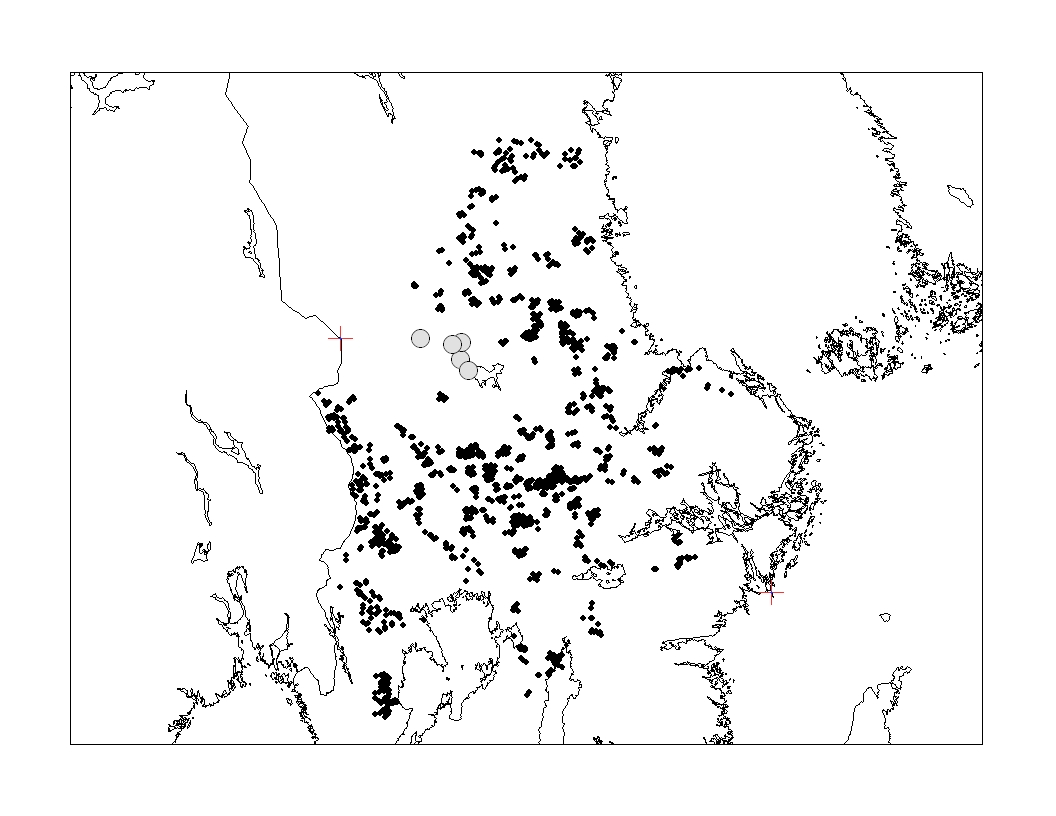
\includegraphics[height=.5\textheight]{figures/20_ForestFinns}
\caption{Distribution of “Forest Finns” (black dots) compared to that of non-delimited uses of definite forms (grey circles). Sources: \citet{Tarkiainen1990}, \citet{Broberg1980}.}
\label{map:16}

\end{figure}

\section{ Reconstructing the grammaticalization path}
\label{sec:3.4}

The extended uses of definite forms that we see in the Peripheral Swedish area represent a kind of development that has not been studied from a typological or diachronic point of view, although, as was noted above, it is not without parallels outside Scandinavia. In historical linguistics, like in evolutionary biology, it is often the case that researchers look in vain for the “missing link”, that is, the crucial intermediate stages in a process of change – instead, the details of the process have to be inferred from what we can observe in the present. This also holds here. From written documentation, we know that the patterns in question go back at least to the 18\textsuperscript{th} and almost certainly to the 17\textsuperscript{th} century, but we can only guess at what happened between the introduction of the suffixed definite article, which probably took place at least half a millennium earlier, and the point in time when the first attestations show up. 

Our guesses need not be totally unqualified, however. Among the uses of the definite forms that are “extended” from the point of view of Central Scandinavian (and for that matter, English), not all are equally exotic – on the contrary, as I have noted above, many if not most languages with definite articles tend to use them more systematically with generic noun phrases than English and Central Scandinavian. We can also observe that the area where we find more generic definites than in the standard languages is larger than that, for example, of the non-delimited uses and the low-referentiality singular count uses. Given these observations, it seems natural to look closer at the possibility that generic uses are the stepping-stone to the latter ones. 

This idea indeed seems to make sense also from the semantic point of view. In fact, genericity has sometimes been used as a collective label for the extended uses: thus, \citet[134]{Hummelstedt1934}, speaks of “allmän eller generell betydelse”,\footnote{ This quotation is difficult to translate since \textit{allmän} and \textit{generell} both mean ‘general’ in Swedish.} \citet[29]{Marklund1976} of “totality meaning” [totalitetsbetydelse] and \citet{BergholmEtAl1999} suggest the term “generic article” as a replacement for Delsing’s “partitive article”. Calling something like \textstyleLinguisticExample{beer} in a sentence such as \textstyleLinguisticExample{He’s drinking beer} “generic” certainly presupposes a rather generous definition of that term, but it has to be admitted that the notion of genericity does not lend itself to an easy delimitation. In the section on generic noun phrases above, I distinguished two basic kinds of generic uses of noun phrases. One of the two basic uses of generic noun phrases discussed in \sectref{sec:3.2.1} was “kind predications”, meaning that something is said about a kind or species rather than about its members, e.g. 

\ea
\gl The northern hairy-nosed wombat is an endangered species. 
\z 

The question that arises is whether it is not possible to say that almost any mention of a species constitutes such a “kind predication”. Indeed, one of the major claims in the influential paper by \citet{Carlson1977} was that “existential” uses of bare nouns in English (as in \textstyleLinguisticExample{There are wolves in the forest}) are really kind-referring. In most contexts, there is in fact no ambiguity between generic and existential readings due to restrictions on the syntactic positions in which these readings can occur. However, there are some seemingly genuine cases of ambiguity, such as \REF{ex:158}, which has one clearly kind-referring reading, which is synonymous to \REF{ex:159}, and one existential, which might occur in a context such as \REF{ex:160}.

\ea\label{ex:158}
\gl \label{bkm:Ref107049066}John studies cats.  
 \z

\ea\label{ex:159} 
\gl \label{bkm:Ref107049087}John studies the species Felis catus.
\z 

\ea \label{ex:160}
\gl \label{bkm:Ref107049114}John studies cats, because he is not allowed to use humans for his experiments. 
\z 

In a language such as French, the two readings of \REF{158} would be distinguished formally, the generic reading taking a definite article and the existential one taking a partitive article. Consider the following quotation from a theological discussion site:

\ea %\label{} 
\langinfo{French}{}{}\\
\gll Peut-on,  par  exemple,  étudier  \textbf{l’} \textbf{ Homme}\\
can-one  for  example  study  \textbf{{\deff} } \textbf{man}\\
\gll sans  étudier  \textbf{des} \textbf{hommes?} \\
without  study.{\inf}  \textbf{P{\art}} \textbf{man.{\pl}} \\
\glt ‘Can one for instance study man without studying human beings?’ (Internet)

\z

These observations notwithstanding, the borderline of genericity is rather fuzzy. I said above that it seems that it is often the construction in which a noun phrase appears that determines whether we understand it as generic or not. But another side of the matter is that one and the same content can often be expressed by alternative constructions, only one of which involves a generic noun phrase. For instance, plain existential statements can be paraphrased as statements involving singular definite generics, e.g.:

\ea
\gl There are not many wombats left.  
 \z

\ea 
\gl The wombat is rare these days.
\z 

\ea 
\gl There are lions in Kenya and Tanzania.
\z 

\ea
\gl The lion is represented in both Kenya and Tanzania. 
\z 

These alternative ways of expressing what is basically the same proposition have parallels in cases such as

\ea
\gl \label{bkm:Ref107116648}I suddenly became dizzy.  
 \z

\ea 
\gl \label{bkm:Ref107116651}A sudden dizziness came upon me.
\z 

where the difference is in whether the state of dizziness is expressed via an adjective or highlighted as an abstract noun \textstyleLinguisticExample{dizziness, }which obtains the role of the subject of the sentence. Semantically, this means that the state is “reified” or “hypostasized”, that is, treated as an abstract object. 

As it turns out, there is considerable cross-linguistic variation in how propositions such as those expressed in \REF{166}{}-\REF{167} are constructed grammatically, and some languages may well choose standard ways of expression that are more similar to \REF{167}. Sympathizers of Whorfianism will see this as evidence of differences in how we structure the world. I am personally somewhat skeptical to such hypotheses, at least as far as fully grammaticalized constructions go. That is, if there is just one standard way of expressing some particular content, more substantial evidence is needed to show that this influences the ways people think. But interesting phenomena are observable when different patterns compete. Consider the following Italian sentence:

\ea %\label{} 
\langinfo{Italian}{}{}\\
\gll Papa  beve  \textbf{il} \textbf{caffè} ogni  mattina.\\
father  drink.{\prs}.3{\sg}  \textbf{{\deff}} \textbf{coffee} every  morning\\
\glt ‘Father drinks coffee every morning.’ (Internet)

\z

In English or Swedish, using definite marking on ‘coffee’ to express the corresponding content results in a rather weird interpretation (the natural reaction is “what coffee?”). In Italian, on the other hand, it is the article-less alternative that is felt to be weird: Father drinks (an unspecified, and thus unusual amount of) coffee every morning (Pier Marco Bertinetto, personal communication). Thus, the definite article seems to be induced by the fact that coffee is drunk regularly, in more or less specified quantities. 

Similarly, in the following Sicilian sentence (quoted from \citet[413]{BertinettoEtAl2000}, original source: \citet[231]{Skubic1973--74}, and its translation into Italian, the swordfish is, it seems, focused enough to be worth “reifying” by the use of a definite article:

\ea 
	\ea { 
	\langinfo{Sicilian}{}{}\\
	\gll	 Aju  manciatu  tanti  voti  \textbf{u} \textbf{piscispata,}\\
			have.{\prs}.1{\sg}  eat.{\pp}  many  time.{\pl}  \textbf{{\deff}} \textbf{swordfish}\\
	\gll 	e  m’  ha  fattu  sempri  beni.\\
			and  me.{\dat}  have.\textsc{prs.3sg}  do.{\pp}  always  good\\
	}
	\ex {
	\langinfo{Italian}{}{}\\
	\gll 	Ho  mangiato  tante  volte  \textbf{il} \textbf{pesce} \textbf{spada,}\\
			have.{\prs}.1{\sg}  eat.{\pp}  many  time.{\pl}  \textbf{{\deff}} \textbf{fish} \textbf{sword}\\
	\gll 	e  mi  ha  fatto  sempre  bene.\\
			and  me.{\dat}  have.\textsc{prs.3sg}  do.{\pp}  always  good\\
	\glt 	‘I have eaten swordfish many times, and it has always done me well.’
	}
	\z	 
\z

The competition between different grammatical patterns makes it possible for subtle nuances in interpretation to arise (see for further discussion \citealt[128--134]{Dahl2004}). If, on the other hand, the use of the definite article in a similar context becomes obligatory, as in the Peripheral Swedish vernaculars, such nuances are lost. Another point to be made in this connection is that usage is often regulated in specific constructions but the way it is regulated may vary from one language to another. Consider, as an example, complements of verbs like \textstyleLinguisticExample{smell}, as in

\ea
\gl He smells of vodka.  
 \z

%\end{listLFOileveli}

In most Germanic languages, it is simply impossible to use definite marking here, and from this point of view, it may seem more plausible to construe such sentences as talking of a restricted quantity of vodka, rather than as involving a kind predication in the sense of \citet{KrifkaEtAl1995}. Nevertheless, in many Peripheral Swedish varieties as well as in French, the normal construction is with a definite article: 

\ea %\label{} 
\ea {
\langinfo{Älvdalen (Os)}{}{}\\
\gll An  lupter  \textbf{brendwineð}\\
he  smell.{\prs}  \textbf{vodka.{\deff}}\\
}
\ex {
\langinfo{French}{}{}\\
\gll Il  sent  \textbf{la} \textbf{vodka}\\
he  smell.{\prs}.3{\sg}  \textbf{{\deff}} \textbf{vodka}\\
\glt ‘He smells of vodka.’
}
\z 
\z

This could be interpreted as evidence that Elfdalian and French construe the predicate ‘smell’ as holding between a perceiver and a kind, and that other languages construe it as holding between a perceiver and an indefinite quantity of something. On the other hand, since there is no evidence for such a cognitive difference, it could be argued that it is equally plausible that languages are indifferent to the distinction between these two possible construals. 

The Romance languages, which on the whole seem more generous than Germanic in allowing definite articles in the fuzzy border area of genericity, exhibit some interesting cross-linguistic patterns of variation. \citet{Zamparelli2002} discusses various examples of what looks like extended uses of definite articles in Italian and other Romance languages. According to him, the following cases “force us to conclude that, in Italian, some definites can … have a purely indefinite meaning”. (The glosses in \REF{173}{}-\REF{178} and \REF{182}{}-\REF{184} are Zamparelli’s. The boldface is mine.)

\ea %\label{} 
\langinfo{\label{bkm:Ref172696600}\label{bkm:Ref69030048}Italian}{}{}\\
\gll Ogni  settimana,  {il mio}  {sito web} viene  attaccato  dagli  hacker.\\
every  week,  my  web\_site is  attacked  by\_{\deff}.{\pl}  hacker\\
\glt ‘Every week, my web site is attacked by \textbf{the hackers}.’
\z

\ea %\label{} 
\langinfo{\label{bkm:Ref69030716}Italian}{}{}\\
\gll Nel  1986  \textbf{i} \textbf{ladri} hanno  svuotato {il mio}  appartamento.\\
In  1986  \textbf{{\deff}} \textbf{thieves} have  emptied my  apartment.\\
\glt ‘In 1986 the thieves emptied my apartment.’
\z

\ea %\label{} 
\langinfo{Italian}{}{}\\
\gll La  casa  è  sporchissima.\\
{\deff}  house  is  filthy.\\
\gll In { } cantina  ci  sono  \textbf{i} \textbf{topi} e  sotto  il  lavello  vivono  \textbf{gli} \textbf{scarafaggi}.\\
In {\deff}  basement  there  are  \textbf{{\deff}} \textbf{mice} and  under  {\deff}  sink  live  \textbf{{\deff}} \textbf{cockroaches}\\
\glt ‘The house is filthy. In the basement there are the mice and under the sink live the cockroaches.’  

\z

\ea %\label{} 
\langinfo{Italian}{}{}\\
\gll Che  fai  per  mestiere?  Fotografo  \textbf{gli} \textbf{uccelli}.\\
What {do you  do}  for  {{\indf} living}?  {I photograph}  \textbf{{\deff}} \textbf{bird.{\pl}}\\
\glt ‘What do you do for a living? I photograph the birds.’

\z

\ea %\label{} 
\langinfo{Italian}{}{}\\
\gll Con  questi  disturbi  {ho  dovuto} smettere  di  bere  \textbf{il} \textbf{caffè}.\\
with  this  condition  {I  had to} stop  to  drink  \textbf{{\deff}} \textbf{coffee}.\\
\gll \textbf{Il} \textbf{tè} invece  {mi facilita}  la digestione.\\
\textbf{{\deff}} \textbf{tea} instead  helps  the digestion.\\
\glt ‘With this condition I had to stop drinking the coffee. The tea instead helps my digestion.’

\z

\ea %\label{} 
\langinfo{\label{bkm:Ref172696628}Italian}{}{}\\
	\gll Gianni  è  così  pallido  che  sembra  abbia  visto  \textbf{i} \textbf{fantasmi.} \\
Gianni  is  so  pale  that  {it seems} {he has}  seen  \textbf{{\deff}} \textbf{ghosts}  \\
\gll   \\
 \\
\glt ‘Gianni is so pale that it seems he has seen the ghosts.’
\todo[inline]{tense of gloss and translation should be pluperfect}
\z

Zamparelli’s examples have in common that it is not natural to preserve the definite article when translating into English. They differ from each other in various ways, however. Consider, to start with, \REF{173}. It is not generic in the sense that it is a general statement about hackers. Rather, what it says is that every week, some hackers visit my site. Whether it is the same persons every week or not is not said, and probably the speaker does not know. What could be argued here is that in \REF{173}, the hackers who visit my site are seen as representatives of the world-wide community of hackers, as it were. Similarly, the mice in the basement in \REF{174} could be thought of as representing the mouse species in general. This would make \REF{173} and \REF{174} a bit similar to a sentence such as the following: 

\ea
	\gl \label{bkm:Ref69031158}The Americans have visited the moon.  
\z

\ea 
\gl \label{bkm:Ref77501116}Swedish
\z
 
\ea%\label{}
\gll \textbf{Räven} har  varit  i  hönshuset  igen.\\
\textbf{fox.{\deff}} have.{\prs}  be.{\supp}  in  hen-house.{\deff}  again\\
\glt ‘The fox has been in the hen-house again.’

\z

There are clear differences here though. In English, the conditions for using the definite article in a “representative” sense are stricter than in Italian. It appears that the reason one can say something like \REF{179} is that the American visitors to the moon were representatives of the American nation not only in some extended or metaphorical sense but also quite concretely, since they acted on behalf of the US government. When it becomes possible to go to the moon as a tourist, it clearly will not be sufficient for me and some of my friends to go there for \REF{181} to be true.

\ea
\gl \label{bkm:Ref94431191}The Swedes have visited the moon.  
 \z

	 \REF{180} is different from Zamparelli’s example in that the noun phrase is in the singular. Zamparelli notes that if \textstyleLinguisticExample{il topo} ‘the mouse’ is substituted for \textstyleLinguisticExample{i topi }in \REF{174}\textstyleLinguisticExample{, }the interpretation has to be specific. A prerequisite for the use of a singular in \REF{180} is that foxes tend to operate one by one, in such a way that we can think of the fox that visited the hen-house last night as a representative of the fox species. 

Zamparelli notes that the three Romance languages Italian, Spanish and French differ in how readily they accept definite noun phrases in contexts of this kind. Thus, in the French translation of \REF{174}, only partitive articles are possible. In Spanish, definite articles are possible, but not with the existential verb \textstyleLinguisticExample{hay} ‘there is’, only with verbs such as \textstyleLinguisticExample{estar} ‘be’ and \textstyleLinguisticExample{vivir} ‘live’:

\ea %\label{} 
\langinfo{\label{bkm:Ref172696738}French}{}{}\\
\gll Dans  la  cave,        il  y       a      \textbf{?les} \textbf{/} \textbf{des} \textbf{souris},      et  dans  l’  évier       vivent              ?les    /  des  cafards.\\
     in  {\deff}  basement  it  there  have  \textbf{{\deff}} {}      \textbf{{\partart}} \textbf{mouse.{\pl}} and  in  {\deff}  sink  live.{\prs}.3{\pl}  {\deff}  {}   {\partart}   cockroaches \\
 
\glt ‘In the basement there are the mice and under the sink live the cockroaches.’ 

\z

\ea %\label{} 
\langinfo{Spanish}{}{}\\
\gll En  el  sótano  hay  \textbf{(*los)} \textbf{  ratones,}\\
In  {\deff}  basement  exist  \textbf{({\deff})} \textbf{mice,}\\
\gll y  bajo  la  fregadera  hay  \textbf{(*las)} \textbf{cucarachas}.\\
and  under  {\deff}  fridge  exist  \textbf{({\deff})} \textbf{cockroaches}\\
\glt ‘In the basement there are mice and under the fridge there are cockroaches.’  

\z

\ea %\label{} 
\langinfo{\label{bkm:Ref172696740}Spanish}{}{}\\
\gll En  el  sótano  están  \textbf{*(los)} \textbf{  ratones,}\\
In  {\deff}  basement  are  \textbf{({\deff})} \textbf{mice}\\
\gll y  bajo  la  fregadera  vivon  \textbf{*(las)} \textbf{cucarachas}.\\
and  under  {\deff}  fridge  live  \textbf{({\deff})} \textbf{cockroaches}\\
\glt ‘ In the basement are mice and under the fridge live cockroaches.’  

\z

What we see here, then, is a cline of acceptability for definite noun phrases in uses that can be seen as non-delimited, with French being most restrictive and Italian being most liberal. This then suggests a way by which definite noun phrases may expand their domain of use into the indefinite territory with the situation in the Peripheral Swedish vernaculars or Moroccan Arabic (see \sectref{sec:3.2.3.2} above) as the eventual result. In the absence of historical data, it is of course impossible to verify whether the route has been exactly the same, but given the other circumstances mentioned in the beginning of this section, generic uses must be regarded as a highly probable diachronic source for the extended uses of definite forms. 

For singular count nouns, there are also non-generic uses of definite-marked noun phrases than generic ones that could serve as bridging cases. Consider the following sentences in English:

\ea
\gl \label{bkm:Ref123724733}Did you bring \textbf{the knife}?\\
\z 

\ea 
\gl \label{bkm:Ref123724734}Did you bring \textbf{a knife}?\\
\z 

In many situations, both \REF{185} and \REF{186} would be acceptable. (Imagine, for instance, a picnic.) It is often rather irrelevant if a specific knife is held in mind or not. In Swedish, one could use any of the following three variants:

\ea %\label{} 
\langinfo{Swedish}{}{}\\
\gll Tog  du  med  dig  \textbf{kniven/en kniv/kniv?}\\
take.{\pst}  you  with  you  \textbf{knife.{\deff}/{\indf} knife/knife}\\
\glt ‘Did you bring a knife?’

\z

It thus seems plausible that the fluidity of the use of articles here could set the scene for the expansion of the definite forms. In fact, this fluidity sometimes makes it difficult to evaluate uses of definite markings in written sources. Consider the following excerpt from a recording of a speaker born in 1881 and coming from Hållnäs, one of the linguistically most conservative parishes in Uppland:

\ea %\label{} 
\langinfo{\label{bkm:Ref123725093}Hållnäs (Up)}{}{}\\
{}[The speaker is describing how sheep were collected from their summer-pasture in the autumn.]\\
\gll 	Å  den  såm  hadde  nô  förstånd  då  se  feck\\
		and  he  who  have.{\pst}  some  sense  then  see.{\imp}  get.{\pst}\\
\gll 	han  ju  ha  \textbf{bröy-sättjin,} helle  \textbf{bröy-kôrjin,} å\\
		he  {\prag}  have.{\inf}  \textbf{bread-sack.{\deff}} or  \textbf{bread-basket.{\deff}} and\\
\gll 	le{\textasciigrave}t  åpp  en  ta´ckâ  såm  fåLd  etter.\\
		search.{\inf}  up  {\indf}  ewe  who  follow.{\pst}  after\\
\glt  ‘And he who had some sense got to have the bread sack, or the bread basket, to find a ewe who was lagging behind.’ (\citealt[33]{KällskogEtAl1993})

\z

Speakers of standard Swedish do not react to the use of definite forms here, but if \REF{188} had occurred in a Peripheral Swedish area vernacular, it could relatively easily be seen as parallel to the examples discussed in \sectref{sec:3.2.5}.

Many of the extended uses of definite forms seem rather eccentric from the point of view of standard definitions of definiteness. As was mentioned above, it is a general characteristic of advanced stages of the evolution of definite articles that the semantic element of definiteness is weakened or gets lost entirely, as when articles develop into general affixes on nouns. Such a loss of the semantic essence of a morpheme may appear paradoxical, in that the motivation for having a definite article in the first place ought to be to express definiteness. In the words of \citet[91]{Hawkins2004}, “why should the definite article be recruited for more and more NPs in performance and grammar and gradually jettison the semantic-pragmatic conditions of its deictic source?”  Hawkins suggests that the answer has to be found in the processing of grammar: the functions of definite articles that become dominant at later stages of its evolution are to “construct a (case-marked) NP” and to “attach specified categories to the (case-marked) NP that it constructs”. It is not clear from Hawkins’ text if “construct” means anything but “unambiguously signal”, but the consequence is in any case that the function of a definite article is syntactic rather than semantic. Hawkins notes (quoting \citealt[64]{Lyons1999}) that the cross-linguistic tendency for definite articles to occur early in noun phrases can be explained through the necessity to signal the NP-hood of an expression early on. Notice that the principle “Signal NP-hood as early as possible” would have much of the same effect as the principle “The D-position must be filled” suggested by Holmberg \& Sandström. However, Hawkins’ principle makes most sense in complex NP’s, where an article preposed to or cliticized to the first word would function much as a labeled left bracket. It is less clear what the point of having a definite article on a bare noun would be. Perhaps we should see the function of definite articles whose use is extended beyond what is warranted by semantic definiteness as enhancing the general level of redundancy in grammar and thus making the transmission of the message safer (see \citealt[9--11]{Dahl2004}). It should be added that any theory which attributes too essential a role to definite suffixes in varieties like the Peripheral Swedish ones will have problems explaining the tendency in the same varieties towards extensive neutralization of the distinction between definite and indefinite forms. 

